\documentclass[a4paper, 12pt]{report}

%%%%%%%%%%%%
% Packages %
%%%%%%%%%%%%
\usepackage{rest-api}
\usepackage[english]{babel}
\usepackage[noheader]{packages/sleek}
\usepackage{packages/sleek-title}
\usepackage{packages/sleek-theorems}
\usepackage{packages/sleek-listings}
\usepackage[most]{tcolorbox}


\usepackage{color}
\usepackage{tabularx}

\usepackage{pdfpages}

\definecolor{pblue}{rgb}{0.13,0.13,1}
\definecolor{pgreen}{rgb}{0,0.5,0}
\definecolor{pred}{rgb}{0.9,0,0}
\definecolor{pgrey}{rgb}{0.46,0.45,0.48}
\definecolor{tsyellow}{RGB}{255,185,88}

\usepackage{listings}
\lstset{language=Java,
 columns=fullflexible,
  showspaces=false,
  showtabs=false,
  frame=single,
  breaklines=true,
  postbreak=\mbox{\textcolor{red}{$\hookrightarrow$}\space},
  showstringspaces=false,
  breakatwhitespace=true,
  commentstyle=\color{pgreen},
  keywordstyle=\color{pblue},
  stringstyle=\color{pred},
  basicstyle=\ttfamily
}

\usepackage{enumitem,amssymb}

\newlist{todolist}{itemize}{2}
\setlist[todolist]{label=$\square$}

\newenvironment{boxexercise}
{\begin{tcolorbox}
[enhanced jigsaw,breakable,pad at break*=1mm,
 colback=tsyellow!20,boxrule=0pt,frame hidden]}
{\end{tcolorbox}}

\newenvironment{summary}
{\hspace{10pt}\par\small\it
 \begin{list}{}{\leftmargin=35pt\rightmargin=25pt}
 \item\ignorespaces\advance\baselineskip -1pt}
{\end{list}\vspace{-0.5cm}}

\newenvironment{remark}
{\vspace{0.5cm}\noindent\small\it
 \marginpar{\vspace{-3mm}
\includegraphics[width=1.0cm]{idea}}}
{\vspace{0.5cm}}

\newtheorem{envoefening}{\textbf{Exercise}}[chapter]
\newenvironment{oefening}
               {\begin{boxexercise}\begin{envoefening}}
               {\end{envoefening}\end{boxexercise}}
               
\newcommand*{\xml}[1]{\texttt{<#1>}}

%%%%%%%%%%%%%%
% Title-page %
%%%%%%%%%%%%%%

\logo{./resources/pdf/logo.png}
\institute{Hogeschool PXL}
\faculty{PXL-Digital}
%\department{Department of Anything but Psychology}
\title{Java Advanced 2}
\author{\textit{Author}\\Nele \textsc{Custers}}
%\supervisor{Linus \textsc{Torvalds}}
%\context{Well, I was bored...}
\date{\today}

%%%%%%%%%%%%%%%%
% Bibliography %
%%%%%%%%%%%%%%%%

\usepackage{biblatex}
\addbibresource{./resources/bib/references.bib}

%%%%%%%%%%
% Others %
%%%%%%%%%%

\lstdefinestyle{latex}{
    language=TeX,
    style=default,
    %%%%%
    commentstyle=\ForestGreen,
    keywordstyle=\TrueBlue,
    stringstyle=\VeronicaPurple,
    emphstyle=\TrueBlue,
    %%%%%
    emph={LaTeX, usepackage, textit, textbf, textsc}
}

\FrameTBStyle{latex}

\def\tbs{\textbackslash}

%%%%%%%%%%%%
% Document %
%%%%%%%%%%%%

\begin{document}
    \maketitle
    \romantableofcontents
    

\chapter{Maven}
\label{chap:maven}

\fcolorbox{black}[HTML]{E9F0E9}{\parbox{\textwidth}{%
\noindent \textbf{Learning goals}\\
The junior-colleague
\begin{enumerate}[nolistsep]
\item can explain what Maven is.
\item can describe the 3 build lifecycles of Maven.
\item can explain that each build lifecycle is made up of phases.
\item can explain that each build phase is made up of plugin goals.
\item can identify the project coordinates.
\item can describe the Maven Standard Directory Layout.
\item can explain what a dependency is.
\item can describe the different dependency scopes.
\item can explain what a transitive dependency is.
\item can explain what a dependency tree is.
\item can execute maven commands from CLI.
\item can manage dependencies with Maven.
\item can create a REST endpoint that provides an image or a file.
\item can run code analysis on a Spring boot project (with SonarQube).
\item can fix bugs, vulnerabilities and code smells detected by SonarQube.
\end{enumerate}}}

\section{What is Maven?}

Maven is a tool that can be used for building and managing Java-based projects.
Every Java project requires certain dependencies, which are automatically downloaded when using Maven.

The main objectives of using Maven for developers are:
\begin{itemize}
\item Making the build process easy
\item Providing a uniform build system
\item Providing information about project quality (for example unit test reports)
\item Encouraging better development practices
\end{itemize}

Maven is much more than a build tool.  Maven offers support for automatic source generation,  compiling the source code and test sources, packaging final product(s) for different environments, running health checks and reporting.  Continuous builds, integration, and testing can be easily handled by using Maven. A tool commonly used for creating CI/CD pipelines (continuous integration and continuous delivery) is Jenkins.  Jenkins cannot replace Maven or vice-versa. Jenkins can use Maven as its build tool.  
When Jenkins deploys artifacts to remote repositories, they are usually Maven repositories. 

According to snyk's 2021 JVM ecosystem report \footnote{\url{https://snyk.io/jvm-ecosystem-report-2021/}} Maven is most popular build tool for the Java ecosystem.

\section{Installation and Configuration}

IntelliJ IDEA has in-built support for Maven.  However we want to make Maven available in the command-line interface. Therefore we need to install Maven. 

 \fcolorbox{black}[HTML]{ADD8E6}{\parbox{\textwidth}{%
\noindent \textbf{Maven download and documentation pages:}\\
Download page: \url{https://maven.apache.org/download.cgi}\\
Installation instructions: \url{https://maven.apache.org/install.html}
}}

Confirm that Maven is installed correctly by executing \fbox{\strut \$mvn -v} in a terminal window. 

\begin{lstlisting}[language=bash, frame=single]
$ mvn -v
Apache Maven 3.8.2 (ea98e05a04480131370aa0c110b8c54cf726c06f)
Maven home: /usr/local/Cellar/maven/3.8.2/libexec
Java version: 17.0.1, vendor: Oracle Corporation, runtime: /Library/Java/JavaVirtualMachines/jdk-17.0.1.jdk/Contents/Home
Default locale: nl_BE, platform encoding: UTF-8
OS name: "mac os x", version: "11.5.2", arch: "x86_64", family: "mac"
\end{lstlisting}


\section{Maven Standard Directory Layout}

When you create a new Maven project, a directory which name matches the artifactId is generated. This directory is known as the project’s base directory. 
Every Maven project has a file named \textbf{pom.xml} which is known as the \textbf{Project Object Model} (POM). This file describes the project, configures plugins, and declares dependencies.
The project’s source code and resources are placed in the folder \textbf{src/main}.
The project’s unit tests are located in \textbf{src/test}.
The target folder is the Maven default output folder. You can delete all the target's folder content with the \fbox{\strut \$mvn clean} command.


\section{Maven architecture}

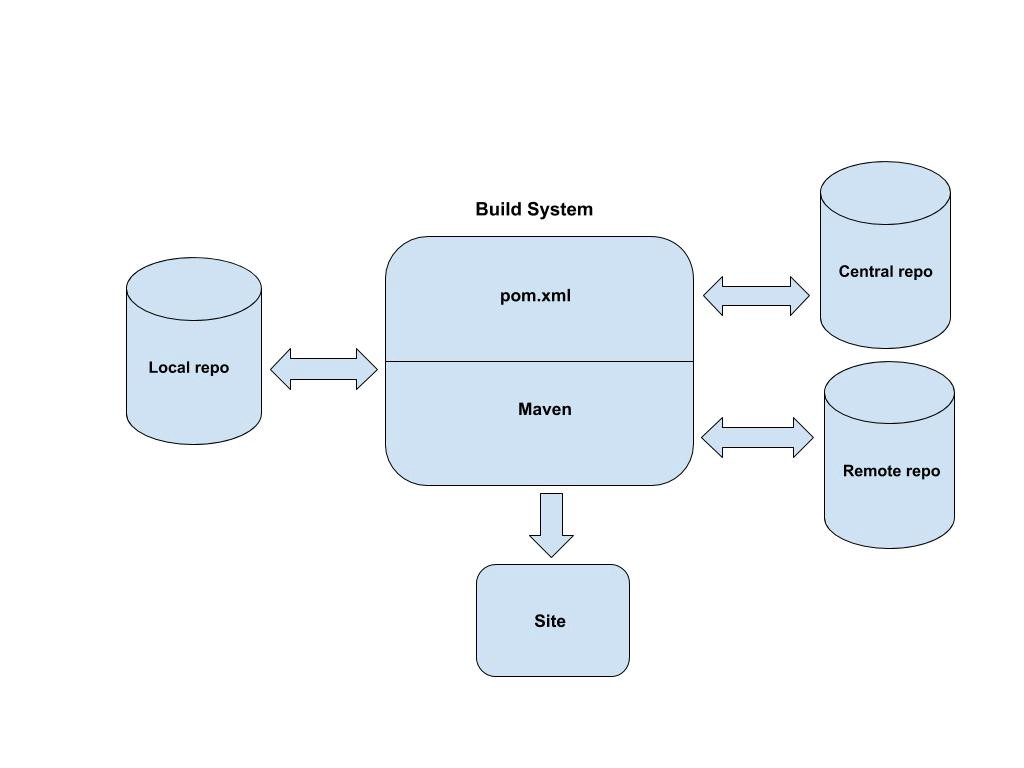
\includegraphics[width=\textwidth]{./images/chapter3/maven-architecture} 

Central repository is provided by the Maven community. This Central repository contains a large number of common libraries.  Whenever you specify a dependency in pom.xml,  Maven will look for it in the local repository first. If the necessary dependency  isn't included in the local repository, Maven will download it from the Central repository and copy it to your local repository.  Remote repository is a place where developers (or Jenkins) can copy the final packages, so other developer can use these final packages as a dependency in their projects.

Acces to internet is recommended when using Maven, however it is possible to work offline if all dependencies are available in your local repository.


\section{Maven built-in life cycles}

There are three built-in life cycles defined in Maven.  The \textit{default} build life cycle is the main build life cycle.

\begin{tabularx}{\textwidth}{ |l|X|l| } 
\hline
clean & handles the cleanup of directories and files generated during the build process & mvn clean \\ 
default & handles the build and distribution of the project & mvn [plugin:goal]* [phase]* \\ 
site & create project documentation & mvn site \\ 
\hline
\end{tabularx}

To run a specific goal, without executing the entire phase (and the preceding phases) the command \fbox{\strut \$mvn [plugin:goal]} can be used.  Phases on the other hand are executed in a specific order and all the preceding phases are executed as well!

\section{A Build Lifecycle is Made Up Of Phases}

Each life cycle consists of a sequence of phases. The default build lifecycle consists of 23 phases. In the image below the 8 main phases are included. On the other hand, clean lifecycle consists of 3 phases, while the site lifecycle is made up of 4 phases.

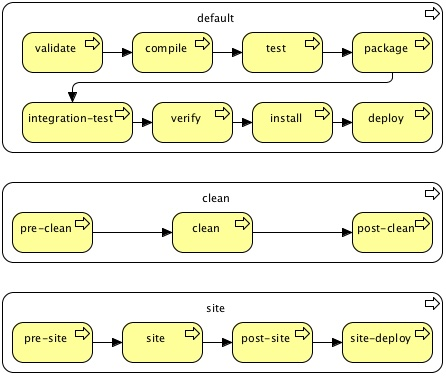
\includegraphics[width=\textwidth]{./images/chapter3/maven-lifecycles} 

Each phase is responsible for a specific task. Here are the 8 most important phases in the default build lifecycle.

\begin{tabularx}{\textwidth}{ |l|X| } 
 \hline
validate & check if all information necessary for the build is available \\
compile & compile the source code \\
test & run unit tests \\
package & package compiled source code into the distributable format, (jar, war, …)\\
integration-test & process and deploy the package if needed to run integration tests \\
verify & run any checks on results of integration tests to ensure quality criteria are met\\
install & install the package to a local repository\\
deploy & copy the package to the remote repository\\
 \hline
\end{tabularx}

\section{Plugins and Goals}

Maven is actually a plugin execution framework. Every task executed by Maven is actually done by a \textbf{goal}, where goals are grouped together in \textbf{plugins}.  When we run a phase, all the goals bound to the phase are executed in order.

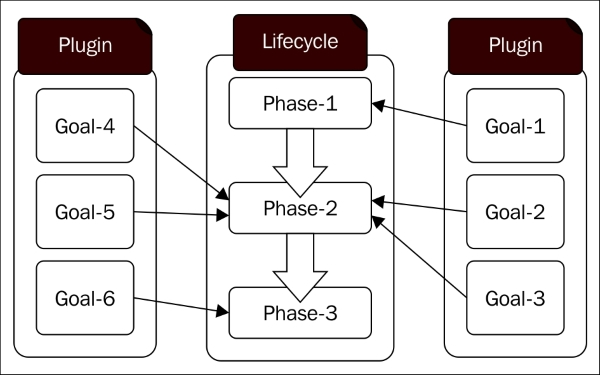
\includegraphics[width=\textwidth]{./images/chapter3/maven_goals} 

Several phases of the default built-in lifecycles have goals bounded to them.  Due to this default configuration you're able to build a Java project without extra configuration.

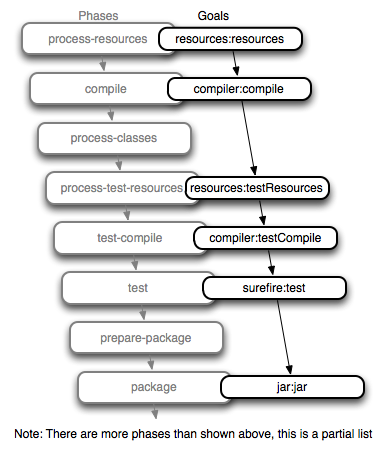
\includegraphics[width=\textwidth]{./images/chapter3/maven-lifecycle-binding} 

The compile goal from the compiler plugin is bound to the compile phase and is responsible for compiling the source code. The test goal from the surefire plugin is bound to the test phase and is reponsible for running the unit tests.

You can generate an overview of all the phases and the specific goals bounded to these phases by running the command \fbox{\strut \$mvn help:describe -Dcmd=PHASENAME}

\begin{lstlisting}[language=bash, frame=single]
$ cd superhero-backend/
$ mvn help:describe -Dcmd=compile
[INFO] Scanning for projects...
[INFO] 
[INFO] ----------------------< be.pxl:superhero-backend >----------------------
[INFO] Building superhero-backend 0.0.1-SNAPSHOT
[INFO] --------------------------------[ jar ]---------------------------------
[INFO]
[INFO] --- maven-help-plugin:3.3.0:describe (default-cli) @ superhero-backend ---
[INFO] 'compile' is a phase corresponding to this plugin:
org.apache.maven.plugins:maven-compiler-plugin:3.1:compile

It is a part of the lifecycle for the POM packaging 'jar'. This lifecycle includes the following phases:
* validate: Not defined
* initialize: Not defined
* generate-sources: Not defined
* process-sources: Not defined
* generate-resources: Not defined
* process-resources: org.apache.maven.plugins:maven-resources-plugin:2.6:resources
* compile: org.apache.maven.plugins:maven-compiler-plugin:3.1:compile
* process-classes: Not defined
* generate-test-sources: Not defined
* process-test-sources: Not defined
* generate-test-resources: Not defined
* process-test-resources: org.apache.maven.plugins:maven-resources-plugin:2.6:testResources
* test-compile: org.apache.maven.plugins:maven-compiler-plugin:3.1:testCompile
* process-test-classes: Not defined
* test: org.apache.maven.plugins:maven-surefire-plugin:2.12.4:test
* prepare-package: Not defined
* package: org.apache.maven.plugins:maven-jar-plugin:2.4:jar
* pre-integration-test: Not defined
* integration-test: Not defined
* post-integration-test: Not defined
* verify: Not defined
* install: org.apache.maven.plugins:maven-install-plugin:2.4:install
* deploy: org.apache.maven.plugins:maven-deploy-plugin:2.7:deploy

[INFO] ------------------------------------------------------------------------
[INFO] BUILD SUCCESS
[INFO] ------------------------------------------------------------------------
[INFO] Total time:  0.896 s
[INFO] Finished at: 2023-02-26T17:19:03+01:00
[INFO] ------------------------------------------------------------------------
\end{lstlisting}


There are two types of plugins:
\begin{itemize}
\item \textbf{Build plugins}: The goals of build plugins are executed during the build process.  If you want to execute additional goals during a phase of the build process, you need to configure the goal in the \xml{build} element of the pom.xml.
\item \textbf{Reporting plugins}: Reporting plugins are executed during the site generation process. These plugins are configured in the \xml{reporting} element of the pom.xml.
\end{itemize}

\section{Dependencies and scopes}

A repository in Maven stores artifacts and dependencies of varying types. There are exactly two types of repositories: local and remote.

The \textbf{local repository} is a directory on the machine that runs Maven.  By default  Maven's local repository is located in the folder \${user.home}/.m2/repository. As you can see, this is a hidden folder.  If you're unable to find the default .m2 folder, you can run the following command:
\fbox{\strut \$mvn help:evaluate -Dexpression=settings.localRepository}

\textbf{Remote repositories} refer to any other type of repository, accessed by a variety of protocols such as file:// and https://. 

\begin{oefening}
Locate and open the folder containing your local repository. 
\end{oefening}

If you're looking for a dependency to add, you can use the Maven Central Repository Search \footnote{\url{https://search.maven.org}}. 

There are two types of dependencies in Maven: direct and transitive. \textbf{Direct dependencies} are the dependencies that are defined in the pom.xml under the \xml{dependencies} section.  \textbf{Transitive dependencies} are dependencies of your direct dependencies.  This means if your project needs dependency A and A depends on B, then your project needs both A and B. However, for Maven it suffices to add dependency A in the pom.xml. The transitive dependency B is included automatically.

You can generate the dependency tree with direct and transitive dependencies by running
 \fbox{\strut \$mvn dependency:tree}.

Sometimes, transitivity brings a very serious problem causing version mismatch issues at runtime.
when multiple versions of the same artifact are encountered, Maven picks the ``nearest definition''. It uses the version of the closest dependency in the dependency tree.

\begin{verbatim}
 A
 \-- B
    \-- C
       \-- D 2.0
 \-- E
    \-- D 1.0
\end{verbatim}

D 1.0 will be used when building project A because the path from A to D through E is shorter. You can explicitly add a dependency to D 2.0 in A to force the use of D 2.0.

\begin{verbatim}
A
 \-- B
    \-- C
       \-- D 2.0
 \-- E
    \-- D 1.0
 \-- D 2.0
 \end{verbatim}

There are 6 dependency scopes which are used to limit the transitivity of dependencies and determine when a dependency should be included in the classpath.

\begin{tabularx}{\textwidth}{ |l|X| } 
 \hline
 compile & 
This is the default scope. Depencencies with this scope are available on the classpath for all the build tasks.\\
provided &
Dependencies that are provided at runtime by JDK or a container. The provided dependencies are available at compile-time and in the test classpath.\\
runtime &
The dependencies with this scope are only required at runtime. They are not needed at compile-time and in the test classpath.\\
test &
These dependencies are only needed for executing tests.\\
system &
Similar to provided but specific jar is provided.\\ 
import &
All dependencies listed in another pom are included.\\
\hline
\end{tabularx}

\section{Exercise}

In the exercise we implement a REST endpoint that returns a PDF file.

\begin{lstlisting}
@GetMapping(value = "/pdfreport", produces = MediaType.APPLICATION_PDF_VALUE)
public @ResponseBody byte[] createPdfReport() {

    ByteArrayInputStream bis = GeneratePdfReport.createReport();

	return bis.readAllBytes();
}
\end{lstlisting}

In the example above we assume to have a helper class GeneratePdfReport that has a method returning a ByteArrayInputStream with the data of your PDF file. We use the @ResponseBody annotation on the controller method to indicate that the object returned by the method should be marshaled directly to the HTTP response body.

For creating PDF files in Java, we'll use itextpdf: \url{https://mvnrepository.com/artifact/com.itextpdf/itextpdf}.

For creating the qr code we will use the ZXing (`Zebra Crossing') API, a popular API for QR code processing in Java. You'll need to include 2 artifacts to be able to generate QR codes.

\begin{lstlisting}
<dependency>
	<groupId>com.google.zxing</groupId>
	<artifactId>core</artifactId>
	<version>3.4.0</version>
</dependency>
<dependency>
	<groupId>com.google.zxing</groupId>
	<artifactId>javase</artifactId>
	<version>3.4.0</version>
</dependency>
\end{lstlisting}

Here is the full code for filling the name and QR code in the PDF template.

\begin{lstlisting}
package be.pxl.superhero.service.impl;

import be.pxl.superhero.api.SuperheroDTO;
import be.pxl.superhero.commons.Cipher;
import com.google.zxing.BarcodeFormat;
import com.google.zxing.WriterException;
import com.google.zxing.client.j2se.MatrixToImageWriter;
import com.google.zxing.common.BitMatrix;
import com.google.zxing.qrcode.QRCodeWriter;
import com.itextpdf.text.DocumentException;
import com.itextpdf.text.Element;
import com.itextpdf.text.Image;
import com.itextpdf.text.Phrase;
import com.itextpdf.text.pdf.ColumnText;
import com.itextpdf.text.pdf.PdfContentByte;
import com.itextpdf.text.pdf.PdfReader;
import com.itextpdf.text.pdf.PdfStamper;
import org.springframework.stereotype.Component;

import java.io.ByteArrayInputStream;
import java.io.ByteArrayOutputStream;
import java.io.IOException;
import java.net.URISyntaxException;
import java.nio.file.Path;
import java.nio.file.Paths;

@Component
public class SuperheroIdCardGenerator {

    public ByteArrayInputStream superheroIdCard(SuperheroDTO superhero) {

        ByteArrayOutputStream out = new ByteArrayOutputStream();

        try {
            Path path = 
                Paths.get(ClassLoader.getSystemResource("superheroidcard.pdf").toURI());
            PdfReader pdfReader = new PdfReader(path.toUri().toURL());
            PdfStamper pdfStamper = new PdfStamper(pdfReader, out);
            PdfContentByte canvas = pdfStamper.getOverContent(1);
            ColumnText.showTextAligned(canvas, Element.ALIGN_LEFT, new Phrase(superhero.firstName() + " " + superhero.lastName()), 200, 620, 0);
            ColumnText.showTextAligned(canvas, Element.ALIGN_LEFT, new Phrase(superhero.superheroName()), 200, 550, 0);
            byte[] qrCodeImage = getQRCodeImage(Cipher.skipALetter(superhero.superheroName()), 130, 130);
            Image qrCode = Image.getInstance(qrCodeImage);
            qrCode.setAbsolutePosition(190, 360);
            canvas.addImage(qrCode);
            pdfStamper.close();
            pdfReader.close();
        } catch (DocumentException | URISyntaxException | IOException | WriterException ex) {
            // TODO: add logging - see next chapter
            throw new PdfCreationException(ex);
        }
        return new ByteArrayInputStream(out.toByteArray());
    }

    public static byte[] getQRCodeImage(String text, int width, int height) throws WriterException, IOException {
        QRCodeWriter qrCodeWriter = new QRCodeWriter();
        BitMatrix bitMatrix = qrCodeWriter.encode(text, BarcodeFormat.QR_CODE, width, height);

        ByteArrayOutputStream pngOutputStream = new ByteArrayOutputStream();

        MatrixToImageWriter.writeToStream(bitMatrix, "PNG", pngOutputStream);
        return pngOutputStream.toByteArray();
    }
}
\end{lstlisting}

The PdfReader first opens the PDF template file. The PdfStamper is used for adding the full name, the alias and the
QR code (as an image) to the template. The newly generated PDF is returned as a ByteArrayInputStream.

\begin{oefening}

All superheroes need an id card. Your job as a developer is to create a REST endpoint where we can download a pdf with the id card.

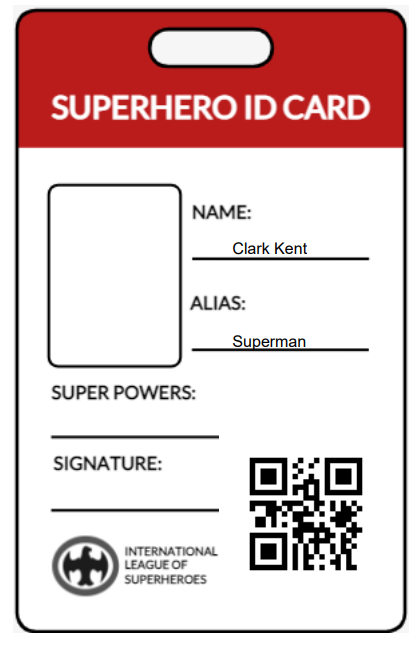
\includegraphics[width=5cm]{./images/chapter3/superhero_id_card.png}

The pdf template can be found in blackboard. 

$\square$ Download the pdf template and add it to the resources directory of your superhero-backend project.

\vspace{5mm}

We will include the full name, the superhero name and a unique QR code in the template.
The generated pdf will be available at the endpoint:
\url{http://localhost:<port>/api/superheroes/<superheroId>/idcard}

The QR code will contain the scrambled alias of a superhero. 

\vspace{5mm}

$\square$ Create the utility class Cipher with a static method skipALetter which takes a String as a parameter and returns the scrambled String. To encrypt a sentence you divide each word into half. If a word has an odd number of letters, the first group of letters contains one letter extra. Take the first letter of the first group, followed by the first letter of the second group. Then, write the second letter of the first group and the second letter of the second group, and so on, until all the words are encrypted. For example, if your sentence is `SECRET CODES', it will be encrypted as `SREECT CEOSD'.

Write unit tests to test your implementation. 
\begin{itemize}
\item unit test for one word with even length
\item unit test for one word with odd length
\item unit test for a sentence with multiple words with odd and even length
\item unit test for an empty string (should return an empty string)
\end{itemize}

\vspace{5mm}

$\square$ Implement the REST endpoint for retrieving a superhero's id card.  
\end{oefening}

\section{Code quality with SonarQube}

We would like to deliver high quality Java code. SonarQube is a Java analyzer that checks the quality of our code and detects code smells.

\begin{oefening}

Create a docker container with SonarQube. Run the following command in a terminal window:

\fbox{\strut docker run -d -{}-name sonarqube -p 9000:9000 -p 9092:9092 sonarqube}

Open \url{http://localhost:9000} in a browser. You can login with the default username `admin' and password `admin'. Next you have to update the default password (you have to choose a new password!).

\vspace{5mm}

Create a new SonarQube project for the superhero-backend application. Click on the button `Manually', fill out the project details and choose to analyze your project locally. A token will be generated.

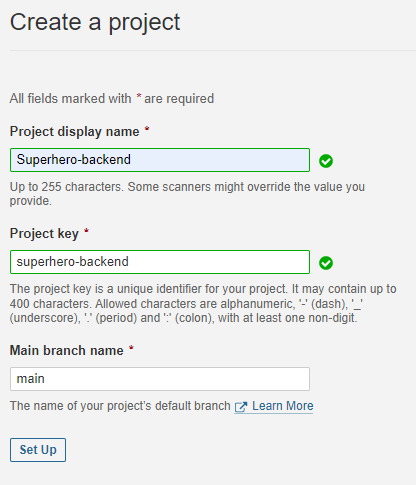
\includegraphics{./images/chapter3/sonarqube_create_project.png}

Now we can update the pom.xml file of our superhero-backend to run the code analysis.

First we need a sonar profile to provide the url, project key and token.

\begin{lstlisting}
<profiles>
	<profile>
		<id>sonar</id>
		<activation>
			<activeByDefault>true</activeByDefault>
		</activation>
		<properties>
			<sonar.host.url>http://localhost:9000</sonar.host.url>
			<sonar.projectKey>superhero-backend</sonar.projectKey>
			<sonar.login>sqp_6319ae2795ccdc24baa3a994962a8bbaa0b0cc16</sonar.login>
		</properties>
	</profile>
</profiles>
\end{lstlisting}

Run the following maven command to perform the code analysis:
\fbox{\strut \$mvn clean verify sonar:sonar}

\vspace{5mm}

Open the SonarQube dashboard \url{http://localhost:9000/dashboard?id=superhero-backend} to get an overview of possible bugs, vulnerabilities and code smells.
You can get a more in-depth explanation of the code quality rules including examples at \url{https://rules.sonarsource.com/java}. Namely, \url{https://rules.sonarsource.com/java/RSPEC-5786} is an interesting code smell to look at.

\vspace{5mm}

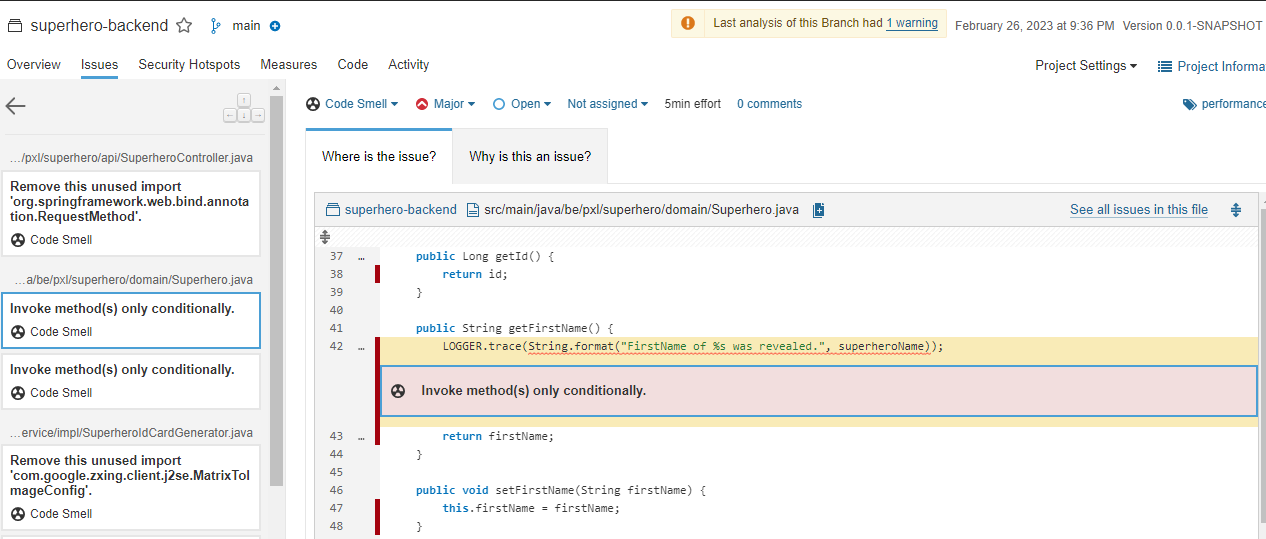
\includegraphics[width=\textwidth]{./images/chapter3/sonarqube.png}

When you look at the dashboard, you'll see the code coverage is always 0.0\%. JaCoCo is needed to generate an extra report to display the code coverage.

First add the property jacoco.version in the pom.xml file:

\begin{lstlisting}
<properties>
	<java.version>17</java.version>
	<jacoco.version>0.8.7</jacoco.version>
</properties>
\end{lstlisting}

Next, add the JaCoCo maven plugin to your project.

\begin{lstlisting}
<build>
	<plugins>
		<plugin>
			<groupId>org.jacoco</groupId>
			<artifactId>jacoco-maven-plugin</artifactId>
			<version>${jacoco.version}</version>
			<executions>
				<execution>
					<id>prepare-agent</id>
					<goals>
						<goal>prepare-agent</goal>
					</goals>
				</execution>
				<execution>
					<id>report</id>
					<phase>test</phase>
					<goals>
						<goal>report</goal>
					</goals>
				</execution>
			</executions>
		</plugin>
	</plugins>
	<pluginManagement>
		<plugins>
			...
		</plugins>
	</pluginManagement>
</build>
\end{lstlisting}

During the test phase JaCoCo will generate a report and save it in the directory target/site/jacoco/jacoco.xml. SonarQube will automatically check this location and the report will be picked up.
First remove the empty, automatically created Spring Boot test from your test folder.
Run the Maven command again and check your code coverage.

\end{oefening}

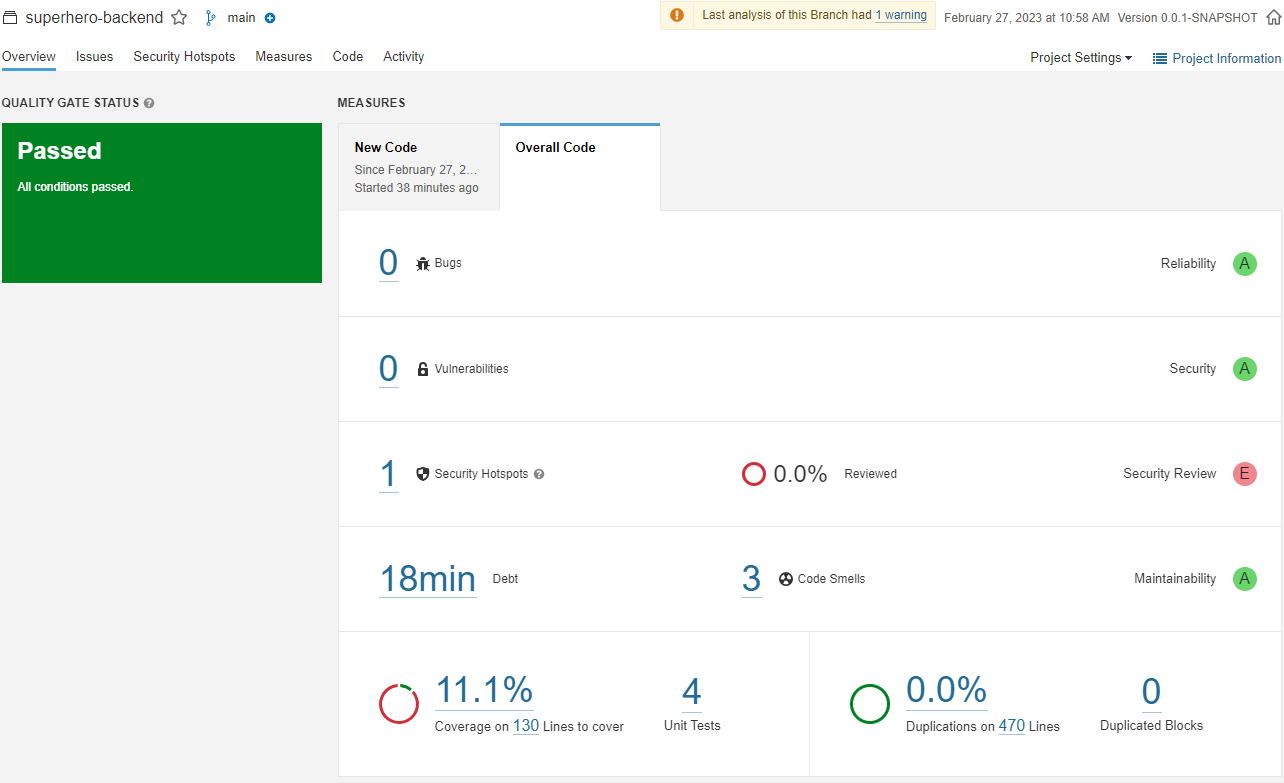
\includegraphics[width=\textwidth]{./images/chapter3/sonarqube-report.png}

\section{Maven commands}

Here is a brief list of usefull Maven commands.

\begin{tabularx}{\textwidth}{ |l|X| } 
\hline
\textbf{Maven Command}	& \textbf{Description} \\
\hline
mvn -v	& Prints out the version of Maven you are running.\\ 
mvn --version & Same as mvn -v\\
mvn clean	& Clears the target directory into which Maven normally builds your project.\\
mvn package & Builds the project and packages the resulting JAR file into the target directory.\\
mvn package -DskipTests &	Builds the project and packages the resulting JAR file into the target directory without running the unit tests during the build. You can also use -Dmaven.test.skip=true\\
mvn clean package &	Clears the target directory,  builds the project and packages the resulting JAR file into the target directory.\\
mvn install & Builds the project described by your Maven POM file and installs the resulting artifact (JAR) into your local Maven repository.\\
mvn -X package & Prints the maven version and runs the build in the debug mode. \\
mvn -o package & This command is used to run the maven build in the offline mode.\\
mvn -help & Prints the Maven usage and all the available options.\\
mvn dependency:tree & Generates the dependency tree of the Maven project.\\
\hline
\end{tabularx}



\chapter{Generics}
\label{chap:generics}

\fcolorbox{black}[HTML]{E9F0E9}{\parbox{\textwidth}{%
\noindent \textbf{Learning goals}\\
The junior-colleague
\begin{enumerate}[nolistsep]
\item can explain what generics is.
\item can describe type erasure and the consequences of type erasure
\item can use generic classes, methods and interfaces
\item can create generic classes, method and interfaces
\end{enumerate}}}

\begin{summary}
Java Generics provides the ability to write generic code that is independent of a data type. When a developer uses a generic class,  interface,  or method,  he will specify which data type will acutally be used. The Java Collections framework is entirely written generically. The moment you use an ArrayList,  you need to indicate the data type for the elements of your list.
\end{summary}

\section{Before generics}
Java is a strongly typed programming language.  During the compilation of a program, you will be pointed out if you use the wrong data type.

\begin{lstlisting}
Object aReference = new Movie("Brother Bear");
Integer luckyNumber = aReference;
\end{lstlisting}

The second line of code results in a compilation error.

 

When Java was introduced, this datatype check was not implemented in the Java Collections framework. The following code compiles without errors.  As soon as you execute the program, an exception will occur.

\begin{lstlisting}
import java.util.ArrayList;
import java.util.Iterator;

public class BeforeGenerics {

	public static void main(String[] args) {
		ArrayList objecten = new ArrayList();
		objecten.add(1);
		objecten.add(5.4);
		objecten.add(new Movie("Inception"));

		Iterator iterator = objecten.iterator();
		double total = 0;
		while (iterator.hasNext()) {
			total += (Double) iterator.next();
		}
		System.out.println(total);
	}
}
\end{lstlisting}


\begin{verbatim}
Exception in thread "main" java.lang.ClassCastException: class java.lang.Integer 
cannot be cast to class java.lang.Double (java.lang.Integer and java.lang.Double 
are in module java.base of loader 'bootstrap')
	at be.pxl.ja.BeforeGenerics.main(BeforeGenerics.java:24)
\end{verbatim}

Type-safety was introduced in the Java Collections framework since Java 5. 
When you open the java documentation for the class java.util.ArrayList, you will see the generic parameter  $<E>$. 
E is the type-parameter and makes it possible to provide a datatype for the elements of the ArrayList. 

\begin{lstlisting}
/**
 * Resizable-array implementation of the {@code List} interface.  Implements
 * all optional list operations, and permits all elements, including
 * {@code null}. 
 * ...
 * @param <E> the type of elements in this list
 *
 * @author  Josh Bloch
 * @author  Neal Gafter
 * @see     Collection
 * @see     List
 * @see     LinkedList
 * @see     Vector
 * @since   1.2
 */
public class ArrayList<E> extends AbstractList<E>
        implements List<E>, RandomAccess, Cloneable, java.io.Serializable {
        
    transient Object[] elementData;
    
    /**
     * Returns the element at the specified position in this list.
     *
     * @param  index index of the element to return
     * @return the element at the specified position in this list
     * @throws IndexOutOfBoundsException {@inheritDoc}
     */
    public E get(int index) {
        Objects.checkIndex(index, size);
        return elementData(index);
    }
    
    E elementData(int index) {
        return (E) elementData[index];
    }
    
    ...
}
\end{lstlisting}

\begin{lstlisting}
import java.util.ArrayList;
import java.util.Iterator;

public class SinceGenerics {

	public static void main(String[] args) {

		ArrayList<Double> objecten = new ArrayList<>();
		objecten.add((double) 1);
		objecten.add(5.4);
		//objecten.add(new Movie("Inception"));

		Iterator<Double> iterator = objecten.iterator();
		double total = 0;
		while (iterator.hasNext()) {
			total += iterator.next();
		}
		System.out.println(total);
	}
}
\end{lstlisting}

If you were to add a Movie-object to an ArrayList that accepts Double-objects, you get a compile error.

\begin{verbatim}
Error:(16, 30) java: incompatible types: be.pxl.ja.streamingservice.model.Movie 
cannot be converted to java.lang.Double
\end{verbatim}

When calling the constructor of a generic class, we use the diamond operator $<>$. The compiler can infer the datatype of the objects in the ArrayList (this is called type inference).  We don't need to repeat the datatype when calling the constructor and use the diamond operator.


\section{Writing generic classes}

The generic class Duo  contains a pair of objects of the generic datatype T.  The class definition identifies this class as a generic class by using the type parameter T (<T>).  In the Duo class, you can use T as the datatype for fields,  parameters,  and returntype.

\begin{lstlisting}
public class Duo<T> {
	private T first;
	private T second;

	public Duo(T first, T second) {
		this.first = first;
		this.second = second;
	}

	public T getFirst() {
		return first;
	}

	public T getSecond() {
		return second;
	}
}
\end{lstlisting}

At the moment you create objects of the class Duo,  you will indicate which actual datatype the type parameter T should be replaced with.  For a developer, it looks like the type parameter T is replaced by the chosen datatype.


\begin{lstlisting}
public class DifferentDuos {

	public static void main(String[] args) {
		Duo<String> cocktail = new Duo<>("gin", "tonic");
		System.out.println(cocktail.getFirst());
		Duo<Actor> famousDuo = new Duo<>(new Actor("Ben","Stiller"), new Actor("Owen", "Wilson"));
		Duo<Integer> numbers = new Duo<>(5, 12);
	}

}
\end{lstlisting}

\subsection{Naming conventions}

To avoid confusion between actual classes and generic type parameters in Java, it is important to use correct naming conventions. We will always use a single uppercase letter to name a type parameter.   According to the code conventions, you should never use a single uppercase letter as the name for a class; you must always use meaningful class names. Therefore, when you see a single uppercase letter in Java code, you may assume it is a generic parameter.

We adhere to the following guidelines:

\begin{itemize}
\item E – Element (used in the Java Collections Framework)
\item K – Key (used in Map)
\item N – Number
\item T – Type
\item V – Value (used in Map)
\item S,U,V etc. – use when T already in use
\end{itemize}

\section{Generic interfaces}

\subsection{Interface $Comparable<T>$}

The generic interface $Comparable<T>$ makes it possible to compare objects. 

Once a class implements this $Comparable<T>$ interface, you can use methods like Collections.sort(...) to sort a collection containing objects of this class. We call this ordering the natural order of the class.

When a class implements the $Comparable<T>$ interface, you fill in the type parameter T with the class itself. You must implement the method \textit{int compareTo(T e)}. Through the implementation of this method, you can compare any object of the class with another object of the same class. The int compareTo(T e) method returns:
\begin{itemize}
\item 0 if both objects are equal.
\item -1 or a negative number if this is less than the argument.
\item 1 or a positive number if this is greater than the argument.
\end{itemize}

Always try to keep the natural order of a class consistent with the implementation of equals()-method.  So, when e1.compareTo(e2) == 0, e1.equals(e2) and e2.equals(e1) should also return true.  Null does not belong to any class, so e1.compareTo(null) should always throw a NullPointerException.

\begin{figure}[H]
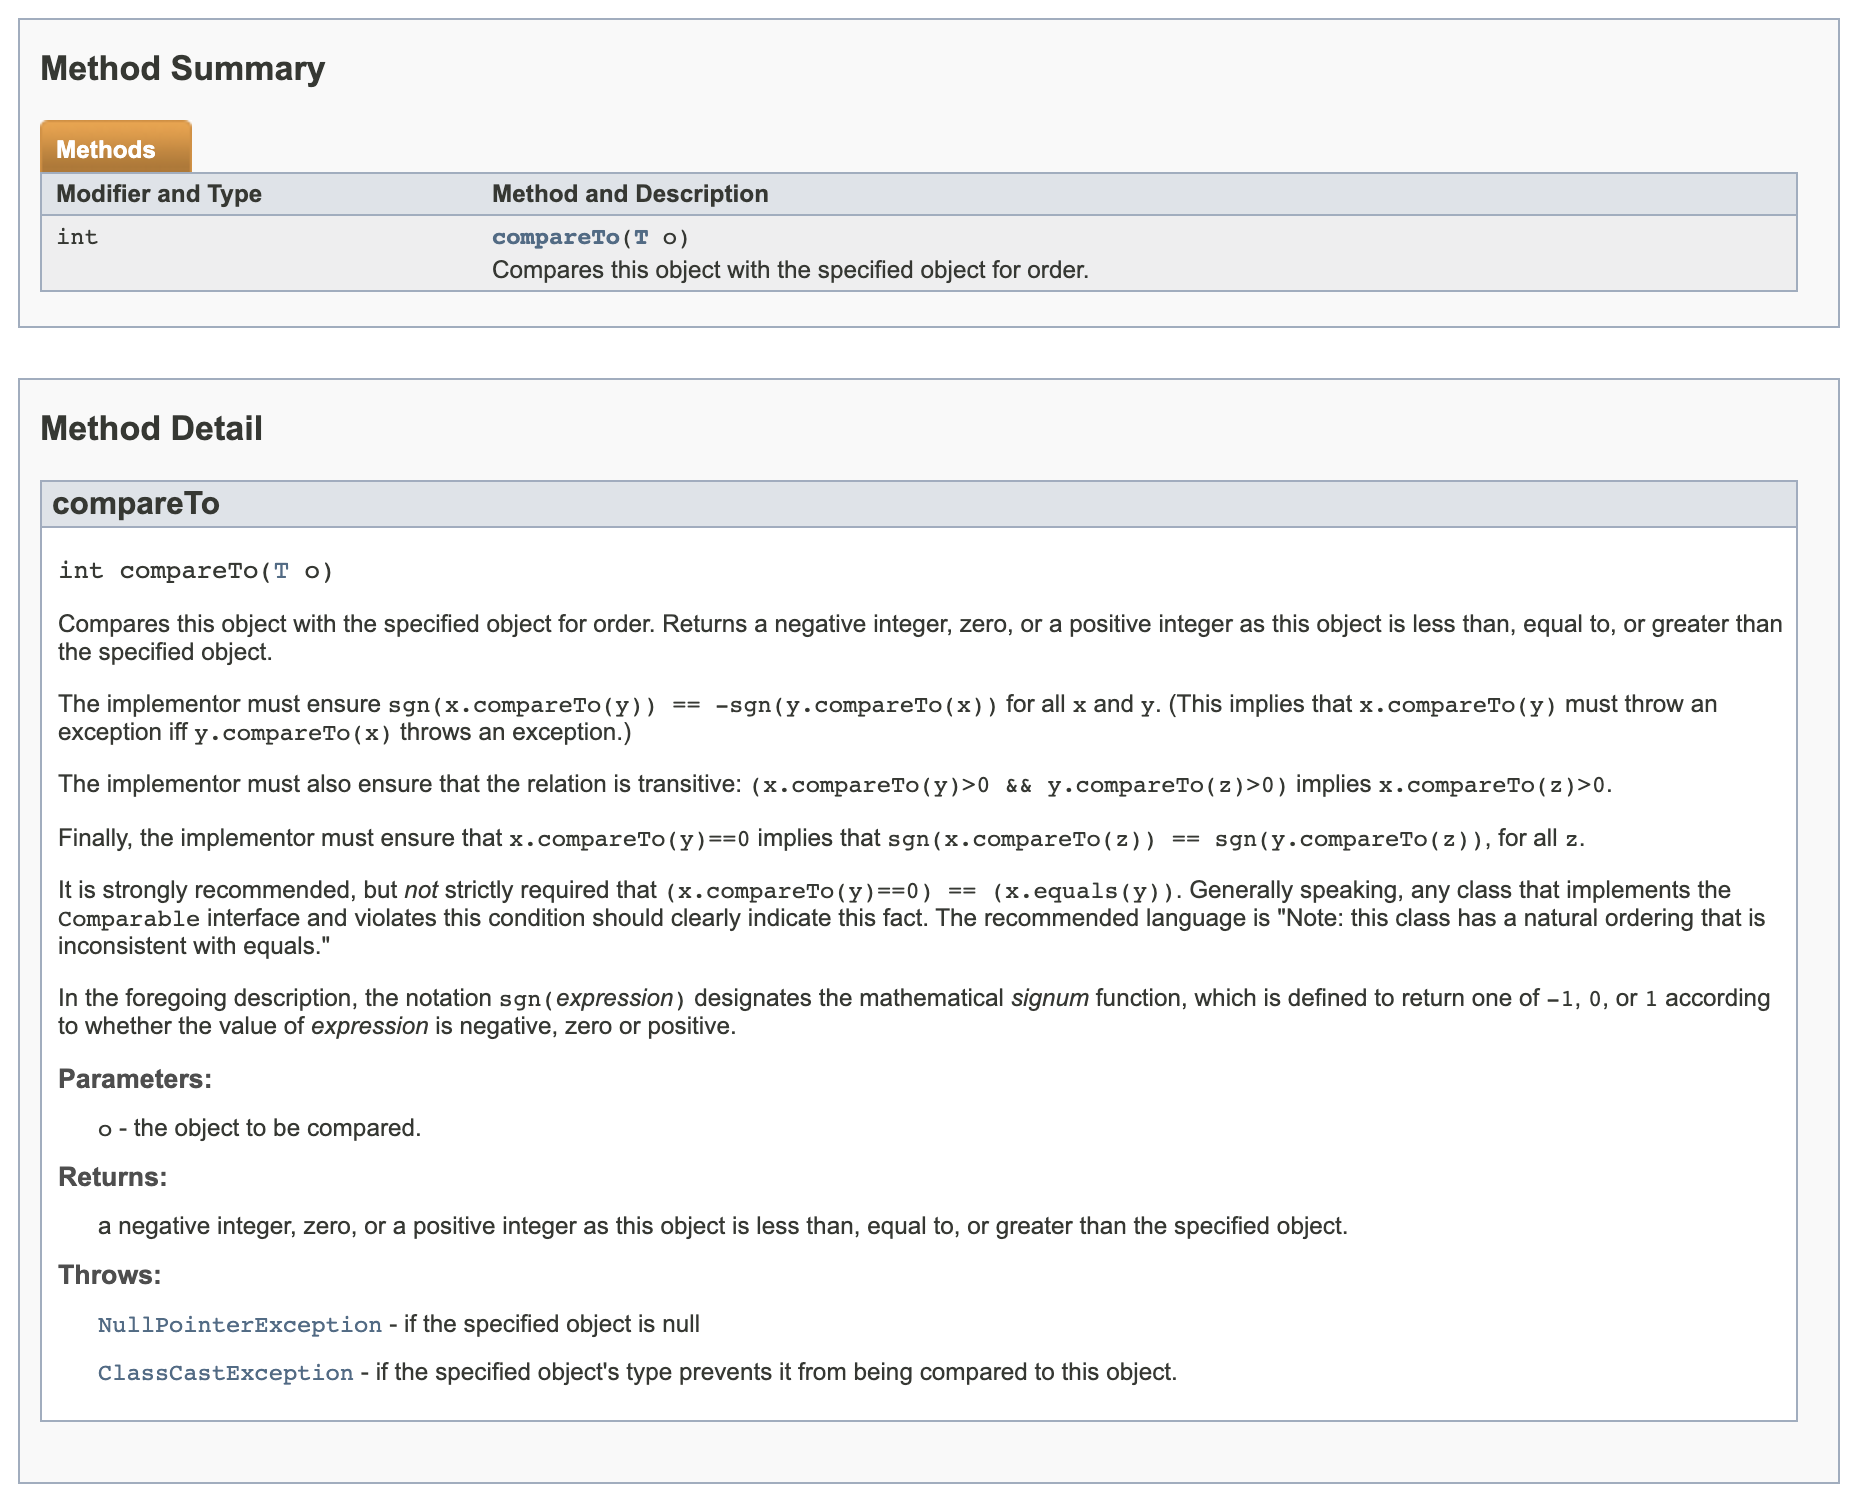
\includegraphics[width=\linewidth]{images/chapter_generics/javadoc_compareTo.png}
\caption{Documentation for interface $Comparable<T>$}
\label{fig:core_classes}
\end{figure}

The class Person has a natural ordering based on the name of a Person-object.  Objects of the class Person can be sorted alphabetically by name. When Person-objects share the same name, we sort by date of birth (younger to older).

\begin{lstlisting}
import java.time.LocalDate;
import java.time.LocalDateTime;
import java.time.temporal.ChronoUnit;
import java.util.Objects;

public class Person implements Comparable<Person> {
	private String name;
	private LocalDate dateOfBirth;

	public Person(String name, LocalDate dateOfBirth) {
		this.name = name;
		this.dateOfBirth = dateOfBirth;
	}

	public int getAge() {
		if (dateOfBirth == null) {
			return 0;
		}
		return (int) ChronoUnit.YEARS.between(dateOfBirth, LocalDateTime.now());
	}
	
	@Override
	public int compareTo(Person other) {
		int nameCompare = this.name.compareTo(other.name);
		if (nameCompare == 0) {
			return other.dateOfBirth.compareTo(this.dateOfBirth);
		}
		return nameCompare;
	}

	public String getName() {
		return name;
	}

	@Override
	public boolean equals(Object o) {
		if (this == o) {
			return true;
		}
		if (o == null || getClass() != o.getClass()) {
			return false;
		}

		Person person = (Person) o;

		if (!Objects.equals(name, person.name)) {
			return false;
		}
		return Objects.equals(dateOfBirth, person.dateOfBirth);
	}

	@Override
	public int hashCode() {
		int result = name != null ? name.hashCode() : 0;
		result = 31 * result + (dateOfBirth != null ? dateOfBirth.hashCode() : 0);
		return result;
	}

	@Override
	public String toString() {
		return "Person{" +
				"name='" + name + '\'' +
				", age='" + getAge() + '\'' +
				'}';
	}
}
\end{lstlisting}

\begin{lstlisting}
package be.pxl.demo;

import java.time.LocalDate;
import java.util.ArrayList;
import java.util.Collections;
import java.util.List;

public class SortingPersons {

	public static void main(String[] args) {
		List<Person> persons = new ArrayList<>();
		Person person1 = new Person("Erik", LocalDate.of(1998, 5, 2));
		Person person2 = new Person("Sam", LocalDate.of(2000, 5, 2));
		Person person3 = new Person("Ann", LocalDate.of(2005, 3, 1));
		Person person4 = new Person("Ann", LocalDate.of(2003, 4, 2));
		Person person5 = new Person("Ann", LocalDate.of(2003, 4, 2));

		persons.add(person1);
		persons.add(person2);
		persons.add(person3);
		persons.add(person4);
		persons.add(person5);

		System.out.println(person3.compareTo(person1));
		System.out.println(person4.compareTo(person3));
		System.out.println(person4.compareTo(person5));

		Collections.sort(persons);
		
		System.out.println(persons);
	}
}
\end{lstlisting}


\begin{verbatim}
-4
2
0
[Person{name='Ann', age='18'}, Person{name='Ann', age='20'}, Person{name='Ann', age='20'}, Person{name='Erik', age='25'}, Person{name='Sam', age='23'}]
\end{verbatim}



\subsection{Writing a generic interface}

In addition to generic classes, you can also develop generic interfaces and methods. Here is an example of a generic interface with two generic parameters T and U.

\begin{lstlisting}
public interface Service<T,U> {

	T execute(U arg);
}
\end{lstlisting}

The interface can have different parameter type and returntype, but this is not mandatory. You can, however, choose the same datatype for generic type T and U.

Als je beslist om deze interface te implementeren ben je verplicht om de methode execute te implementeren, maar je ben vrij om het datatype voor de parameter en de return-waarde te kiezen.

Hier volgen 2 klassen die de interface Service implementeren.

\begin{lstlisting}
public class CountService implements Service<Integer, String> {

	@Override
	public Integer execute(String arg) {
		return arg.length();
	}
}
\end{lstlisting}

\begin{lstlisting}
public class PersonConverterService implements Service<String, Person> {
    private static final DateTimeFormatter FORMATTER = DateTimeFormatter.ofPattern("dd/MM/yyyy");
    @Override
    public Person execute(String arg) {
        // Assuming the input format is "Name, Age"
        String[] parts = arg.split(",");
        if (parts.length != 2) {
            throw new IllegalArgumentException("Invalid input format: " + arg);
        }
        try {
            LocalDate dateOfBirth = LocalDate.parse(parts[1].trim(), FORMATTER);
            return new Person(parts[0].trim(), dateOfBirth);
        } catch (DateTimeParseException e) {
            throw new IllegalArgumentException("Invalid date format: " + arg);
        }
    }
}

public class Main {
    public static void main(String[] args) {
        Service<String, Person> personConverter = new PersonConverterService();
        Person person = personConverter.execute("John Doe, 12/03/2001");

        if (person != null) {
            System.out.println("Converted person: " + person);
        } else {
            System.out.println("Conversion failed.");
        }
    }
}
\end{lstlisting}

This program gives the following output:
\begin{verbatim}
Converted person: Person{name='John Doe', age='22'}
\end{verbatim}


\section{Generic methods}

If you don't need a fully parameterized class, it's also possible to create generic methods. Both regular and static methods can contain one or more generic types. Even a constructor can use generic parameters.

Here's an example.
The following static method \textit{occursExactTimes} returns true if the specified item occurs exactly the given number of times in the List. If not, it returns false.
Before the returntype of the method, you have to identify all the generic types that are used in the method.
 
\begin{lstlisting}
import java.util.List;

public class OccurenceUtil {

	public static <T> boolean occursExactTimes(List<T> items, T item, int times) {
		int count = 0;
		for (T anItem : items) {
			if (anItem.equals(item)) {
				count++;
			}
		}
		return count == times;
	}

}
\end{lstlisting}

The method \textit{occursExactTimes} can be used with different datatypes. 

\begin{lstlisting}
import java.util.Arrays;
import java.util.List;

public class Main {

	public static void main(String[] args) {

		List<Integer> numbers = Arrays.asList(7, 15, 23, 12, 8, 7, 23, 13, 32, 7);
		System.out.println(OccurenceUtil.occursExactTimes(numbers, 7, 3));
		System.out.println(OccurenceUtil.occursExactTimes(numbers, 23, 5));
		List<String> animals = Arrays.asList("zebra", "elephant", "kangaroo", "cow", "kangaroo");
		System.out.println(OccurenceUtil.occursExactTimes(animals, "kangaroo", 2));
	}
}
\end{lstlisting}

Executing this program will give you the following output:

\begin{verbatim}
true
false
true
\end{verbatim}



\section{Bounded generics}


Bounded means here \'restricted\', and we can restrict the datatypes that a method accepts.  Given the following class Card.

\begin{lstlisting}
public enum Suit {
	HEARTS,
	DIAMONDS,
	CLUBS,
	SPADES
}

public enum Rank {
	ACE,
	TWO,
	THREE,
	FOUR,
	FIVE,
	SIX,
	SEVEN,
	EIGHT,
	NINE,
	TEN,
	JACK,
	QUEEN,
	KING
}

public class Card implements Comparable<Card> {
    private final Suit suit;
    private final Rank rank;

    public Card(Suit suit, Rank rank) {
        this.suit = suit;
        this.rank = rank;
    }

    public Suit getSuit() {
        return suit;
    }

    public Rank getRank() {
        return rank;
    }

    @Override
    public String toString() {
        return rank + " " + suit;
    }

    @Override
    public int compareTo(Card other) {
        return this.rank.compareTo(other.rank);
    }
}
\end{lstlisting}

We have a utility class with multiple methods to find the highest value.

\begin{lstlisting}
public class MyUtil {
	static int highest(int a, int b) {
		return Math.max(a, b);
	}
	static double highest(double a, double b) {
		return Math.max(a, b);
	}
	static Card highest(Card a, Card b) {
		return a.compareTo(b) > 0 ? a : b;
	}
}

public class Main {

	public static void main(String[] args) {
		System.out.println(MyUtil.highest(5, 9));
		System.out.println(MyUtil.highest(12.6, -4.6));
		System.out.println(MyUtil.highest(new Card(Suit.HEARTS, Rank.FIVE), new Card(Suit.HEARTS, Rank.SEVEN)));
	}
}
\end{lstlisting}

This program will produce the following output:

\begin{verbatim}
9
12.6
SEVEN HEARTS
\end{verbatim}

Is it possible to write one generic method to decide on the highest value?

Let's rewrite our utility class.  Integer, Double, and Card all implement the Comparable interface. 

\begin{lstlisting}
public class MyUtil2 {

	static Integer highest(Integer a, Integer b) {
		return a.compareTo(b) > 0 ? a : b;
	}

	static Double highest(Double a, Double b) {
		return a.compareTo(b) > 0 ? a : b;
	}

	static Card highest(Card a, Card b) {
		return a.compareTo(b) > 0 ? a : b;
	}
}
\end{lstlisting}

This way we can write a generic method.  The generic method allows for comparisons of any type that implements the Comparable interface. 

\begin{lstlisting}
public class MyUtil2 {

	static <T extends Comparable<T>> T highest(T a, T b) {
		return a.compareTo(b) > 0 ? a : b;
	}
}
\end{lstlisting}


A \'bound\' or restriction is a constraint we impose on the generic type parameter.
In a bound, you can include at most 1 class; there is no restriction on the number of interfaces.  However, the class must always come first in the listing:
\textit{
$<$T extends MyClass \& MyFirstInterface \& MySecondInterface \& MyThirdInterface$>$}.

\section{Wildcards}

In generic code,  the question mark (?),  called the wildcard,  represents an unknown type.

\subsection{Unbounded wildcards}

\begin{lstlisting}
import java.util.Arrays;
import java.util.List;

public class Demo2 {

	public static void main(String[] args) {
		List<Integer> list1 = Arrays.asList(1, 2, 3);
		List<String> list2 = Arrays.asList("one", "two", "three");
		MyUtil.printList(list1);
		MyUtil.printList(list2);
	}
}
\end{lstlisting}

How can you write a generic method to display the elements of a list. 
If you think the following method will do the job, feel free to try:

\begin{lstlisting}
import java.util.List;

public class MyUtil {

	public static void printList(List<Object> list) {
		for (Object element: list) {
			System.out.print(element + " ");
		}
		System.out.println();
	}
}
\end{lstlisting}

However, this wil give a compilation error.

\begin{verbatim}
incompatible types: java.util.List<java.lang.Integer> cannot be converted to java.util.List<java.lang.Object>

Required type: List<Object>
Provided: List<Integer>
\end{verbatim}

Using an unbounded wildcard will do the job. 
\begin{lstlisting}
import java.util.List;

public class MyUtil {

	public static void printList(List<?> list) {
		for (Object element: list) {
			System.out.print(element + " ");
		}
		System.out.println();
	}
}
\end{lstlisting}

Occasionally,  a generic type parameter can be replaced with a wildcard. 
As shown in the example below, secondFunction will give a compile error.  Essentially, as a rule of thumb, you may read data with an unknown data type (thus a wildcard), but you may not write the data.

\begin{lstlisting}
public class Experiment {
    public static <E> void firstFunction(List<E> list) {
        list.add(list.get(0));
    }

    public static void secondFunction(List<?> list) {
        list.add(list.get(0)); // !!!!!!!!!!!!!! won't compile !!!!!!!!!
    }
}
\end{lstlisting}

\subsection{Upper bound wildcards}

\begin{lstlisting}
public static void process(List<? extends Foo> list) { /* ... */ }
\end{lstlisting}

The upper bounded wildcard matches Foo and any subtype of Foo.

\subsection{Lower bound wildcards}


Say you want to write a method that puts Integer objects into a list. To maximize flexibility, you would like the method to work on List<Integer>, List<Number>, and List<Object> — anything that can hold Integer values.

\begin{lstlisting}
public static void addNumbers(List<? super Integer> list) {
    for (int i = 1; i <= 10; i++) {
        list.add(i);
    }
}
\end{lstlisting}


\section{Type Erasure and consequences}

Generics exist only \textbf{at compile time}. During the compilation of Java code,  various additional checks are performed on generic classes to ensure the correct use of data types. Then, when generating the bytecode, all information about the generic data type is simply removed. So,  List<T> is, after some checks and the addition of extra code by the compiler, replaced by List<Object> and List<T extends Person> becomes List<Person>. This is what we call type erasure.  In Java, there will always be only one compiled class (.class file) generated for a generic class.

\begin{lstlisting}
List<Integer> list1 = new ArrayList<>();
List<Float> list2 = new ArrayList<>();
if (list1.getClass() == list2.getClass()) {
	System.out.println("Lists have same class.");
}
\end{lstlisting}

Due to type erasure, it is not possible to create generic static variables in a class. It is also not possible to call a constructor of a generic data type. Furthermore, it is not possible to use the generic data type with the instanceof operator.

\begin{lstlisting}
class Box<T> {
   //compiler error
   private static T value;
   private T t;
   
   public Box() {
      // compiler error
   	  t = new T();
   }

   public void set(T t) {
      this.t = t;
   }

   public T get() {
      return t;
   } 
   
   public boolean test() {
       // compile error
	  return t instanceof T;
   }  
}
\end{lstlisting}

\begin{remark}
More information can be found on pluralsight: \url{https://app.pluralsight.com/player?course=java-generics}. 
\end{remark}


\section{Exercise}

\begin{oefening}
Create an abstract class Player with a member variable name. Provide a constructor with  parameter name
\\
Create 3 subclasses for this abstract class Player: BaseballPlayer, VolleyballPlayer, and SoccerPlayer.
\\
Now create a class Team with the following properties:
\\
\begin{itemize}
\item name (String)
\item played (number of games played)
\item won (number of games won)
\item lost (number of games lost)
\item tied (number of games drawn)
\item members (collection of players)
\end{itemize}

Provide getters.  In the constructor,  you pass the name for the team.
\\

Provide a method \textit{addPlayer} to add a player to the team and a method \textit{numberOfPlayers} to ask for the number of players in the team.
\\
Can you add players of a different type (e.g., BaseballPlayer and SoccerPlayer) to one team? Test it! Make sure this is no longer possible.
\\
Provide the method \textit{matchResult(Team opponent, int ourScore, int theirScore)}. This method ensures that for the team for which the method is called and the opponent, the number of played, won, lost, and drawn matches is increased depending on the values for ourScore and theirScore.
\\
Can you call this method (matchResult) for a team of volleyball players against a team of baseball players? Solve this if necessary, so that this is no longer possible.
\\
Finally, add a method \textit{ranking()}. This returns an integer where the team gets 3 points for each win and 1 point for a draw. Now make sure you can create a collection of Team objects and sort them based on the ranking.
\end{oefening}



    

\chapter{Java I/O}

 
 \begin{summary}
File handling is a fundamental aspect of programming, allowing developers to read from, write to, and manipulate files.  Java provides two primary APIs for file handling—the traditional java.io package and the more recent java.nio package. Understanding these APIs enables Java developers to efficiently manage data stored in files. 
 \end{summary}
 
 \section{Basics of File Handling}
 
A file system manages access to both the content of files and the metadata about those files.  Files are stored in directories.  The files and directories are accessed by specifying paths.  Paths are either absolute or relative:

\begin{itemize}
\item An absolute path is a path relative to the file system’s root directory. It’s expressed as the root directory symbol followed by a delimited hierarchy of directory names that ends in the target directory or file name.
\item A relative path is a path relative to some other directory. It’s expressed similarly to an absolute path but without the initial root directory symbol. In contrast, it’s often prefixed with one or more delimited “..” character sequences, where each sequence refers to a parent directory.
\end{itemize}

\begin{thm}[java.io.File]
        \url{https://docs.oracle.com/en/java/javase/21/docs/api/java.base/java/io/File.html}
    \end{thm}



\begin{lstlisting}
package be.pxl.ja;

public class Demo01 {

	public static final String SEPARATOR = System.getProperty("file.separator");

	public static void main(String[] args) {
		System.out.println("Current operating system: " + System.getProperty("os.name"));
		System.out.println("File separator: " + SEPARATOR);
		System.out.println("User's home directory: " + System.getProperty("user.home"));
		System.out.println("Current working directory: " + System.getProperty("user.dir"));
	}
}
\end{lstlisting}


On some systems,  Java can compensate for differences such as the direction of the file separator slashes in a pathname. For example,  in the current implementation on Windows platforms,  Java accepts paths with either forward slashes or backslashes.
Thus, using forward slashes will make your application system independent.

\begin{lstlisting}
File file = new File("baeldung/tutorial.txt");
\end{lstlisting}


\begin{lstlisting}
import java.io.File;

public class PartitionSpace
{
   public static void main(String[] args)
   {
      File[] roots = File.listRoots();
      for (File root: roots)
      {
         System.out.println("Partition: " + root);
         System.out.println("Free space on this partition = " +
                            root.getFreeSpace());
         System.out.println("Usable space on this partition = " +
                            root.getUsableSpace());
         System.out.println("Total space on this partition = " +
                            root.getTotalSpace());
         System.out.println("***");
      }
   }
}
\end{lstlisting}


Like the legacy File class, Path also creates an object that may be used to locate a file in a file system.


\begin{thm}[java.nio.file.Path]
        \url{https://docs.oracle.com/en/java/javase/21/docs/api/java.base/java/nio/file/Path.html}
    \end{thm}
    





\begin{lstlisting}
// java.io API
boolean fileExists = file.exists();
boolean fileIsFile = file.isFile();
boolean fileIsDir = file.isDirectory();
boolean fileReadable = file.canRead();
boolean fileWritable = file.canWrite();
boolean fileExecutable = file.canExecute();
boolean fileHidden = file.isHidden();

// java.nio API
boolean pathExists = Files.exists(path);
boolean pathIsFile = Files.isRegularFile(path);
boolean pathIsDir = Files.isDirectory(path);
boolean pathReadable = Files.isReadable(path);
boolean pathWritable = Files.isWritable(path);
boolean pathExecutable = Files.isExecutable(path);
boolean pathHidden = Files.isHidden(path);
\end{lstlisting}



TODO 1.  traverse directory
2. Filenamefilter
3. chat between 2 programs?

1. Basics of File Handling
Introduction to File Class: Understanding the java.io.File class for file and directory pathnames.
2. Reading and Writing Files
Streams: Introduce InputStream and OutputStream for reading from and writing to byte streams (e.g., FileInputStream, FileOutputStream).
Readers and Writers: Discuss Reader and Writer for character stream operations (e.g., FileReader, FileWriter).
Buffering: Explain the use of BufferedReader and BufferedWriter for efficient reading and writing.
3. Working with Directories
Directory Operations: Methods for listing files in a directory, creating directories, etc.
4. Advanced File Operations
Random Access File: Usage of RandomAccessFile class for reading and writing to any location in a file.
5. Java NIO Package
Path and Paths: Introduce Path class as an upgrade to java.io.File.
Files Class: Utilizing Files class for file operations like checking, deleting, copying, moving files, reading, and writing.
File Channels: Discuss FileChannel for reading, writing, mapping, and manipulating a file.
Buffers and ByteBuffers: Understanding how data is buffered in NIO.
Asynchronous File I/O: Introduce AsynchronousFileChannel for asynchronous file operations.
6. Exception Handling in File I/O
Try-with-resources: Best practices for handling exceptions and ensuring that files are properly closed using the try-with-resources statement.
Handling IOExceptions: Strategies for handling IOException.
7. Serialization and Deserialization
Object Streams: Using ObjectInputStream and ObjectOutputStream for object serialization.
8. Practical Exercises and Examples
File Copy: Implement a program to copy a file.
File Browser: Create a simple console-based or GUI file browser.
Text File Processing: Read a text file, process its content, and write the output to another file.
9. Best Practices
File Handling Best Practices: Discuss best practices in file handling such as closing resources, handling exceptions, and ensuring efficient data processing.


 
 \section{Toegang tot bestanden en directories}
 
Een bestandsysteem bevat een verzameling van directories of mappen. Iedere directory bevat vervolgens subdirectories en eventueel bestanden.

Het pad naar een bestand, vanaf de root bekeken, is afhankelijk van het besturingssysteem.

\begin{table}[h!]
\centering
\begin{tabularx}{\textwidth}{| l | X |}
 \hline
 Besturingssysteem & Absoluut pad\\ 
 \hline
 Mac OS X & /Users/mark/courses/JavaAdvanced/Car.java \\
 Windows & C:\textbackslash public\textbackslash html\textbackslash javafaq\textbackslash index.html\\
 Unix & /home/mark/courses/slides.pdf \\
 \hline
 \end{tabularx}
 \end{table}
 
Java is platformonafhankelijk. De code om een bestand te lezen op Mac OS X zal dus identiek zijn als op Windows of Unix. Je maakt als ontwikkelaar gebruik van platformonafhankelijke interfaces. De achterliggende implementatie is afgeschermd voor de ontwikkelaar.
 
Laat ons eerst eens kijken naar het scheidingsteken dat we gebruiken om het pad op te bouwen.
Dit scheidingsteken kunnen we opvragen door systeemeigenschappen te gebruiken.  Naast de systeemeigenschap (system property) ``file.separator'' zijn er nog enkele handige waarden die je in je programma kan gebruiken.



Wanneer je dit programma uitvoert op Mac OS X krijg je bijvoorbeeld de volgende output:
\begin{verbatim}
Current operating system: Mac OS X
File separator: /
User's home directory: /Users/mark
Current working directory: /Users/mark/PXL/JavaAdv/JavaIO
\end{verbatim}

En op het Windows besturingssysteem:
\begin{verbatim}
Current operating system: Windows 10
File separator: \
User's home directory: C:\Users\20003575
Current working directory: C:\Users\20003575\Documents\PXL\JavaAdv\JavaIO
\end{verbatim}

Maar nu terug naar onze initi\"ele vraag: Hoe kunnen we het pad naar een directory of bestand samenstellen?

Absolute paden zijn afhankelijk van het besturingssysteem en kunnen dus bugs en problemen veroorzaken. Je moet dus hardgecodeerde, absolute paden vermijden in je programma's. Best stel je paden at runtime samen door gebruik te maken van systeemeigenschappen en input van de gebruiker.

We bestuderen in dit hoofdstuk interfaces en klassen uit \textit{java.io} en \textit{java.nio}. 
We gaan klassen uit de originele \textit{java.io} library gebruiken om bestanden te lezen en te schrijven. De nieuwere library \textit{java.nio} biedt ons een aantal klassen die het werken met bestanden eenvoudiger maken. \textit{nio} staat voor non-blocking IO. Deze non-blocking manier om bestanden te lezen en te schrijven valt buiten de scope van deze cursus.

Starten doen we met een aantal klassen uit het package \textit{java.nio.file}.

\begin{itemize}
\item De klasse \textbf{FileSystem}: stelt het onderliggend bestandssysteem voor en zorgt ervoor dat er Path-objecten gemaakt kunnen worden.
\item De interface \textbf{Path}: wordt gebruikt om een bestand of directory in een bestandssysteem te localiseren.
\item De klasse \textbf{Files}: deze klasse voorziet static methoden om bewerkingen met bestanden en directories uit te voeren.
\end{itemize}

\subsection{De klasse FileSystem en de interface Path}

Een Path-object cre\"eer je door de static methode \textit{of} van de interface Path aan te roepen. 

\begin{figure}[H]
  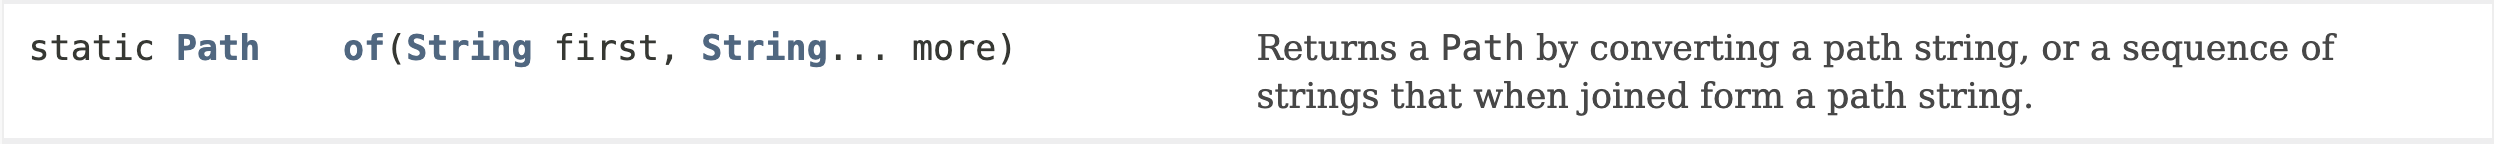
\includegraphics[width=\linewidth]{images/h8/path_of.png}
  \caption{Static methode of in de interface Path}
  \label{fig:paths}
\end{figure}

Achterliggend zal een object van de klasse FileSystem gebruikt worden om Path-objecten te cre\"eeren. FileSystem is wat we noemen een ``factory'' voor Path-objecten. De concrete klasse van een aangemaakt Path-object is afhankelijk van het besturingssysteem.

\begin{lstlisting}
import java.nio.file.FileSystem;
import java.nio.file.FileSystems;
import java.nio.file.Files;
import java.nio.file.Path;

public class Demo02 {

	public static void main(String[] args) {
		FileSystem defaultFileSystem = FileSystems.getDefault();
		System.out.println(defaultFileSystem.getClass());
		for (Path rootDirs: defaultFileSystem.getRootDirectories()) {
			System.out.println(rootDirs);
		}
		Path srcDir = Path.of(System.getProperty("user.dir"), "src");
		System.out.println(srcDir.toAbsolutePath());
		System.out.println(srcDir.getClass().getName());
		System.out.println(Files.isDirectory(srcDir));
	}

}
\end{lstlisting}

Bovenstaand programma geeft volgende uitvoer op een Mac OS X besturingssysteem.

\begin{verbatim}
class sun.nio.fs.MacOSXFileSystem
/
/Users/mark/PXL/JavaAdv/JavaIO/src
sun.nio.fs.UnixPath
true
\end{verbatim}

Volgende uitvoer zal er verschijnen als je het programma uitvoert op een Windows besturingssysteem.

\begin{verbatim}
class sun.nio.fs.WindowsFileSystem
C:\
D:\
C:\Users\20003575\Documents\PXL\JavaAdv\JavaIO\src
sun.nio.fs.WindowsPath
true
\end{verbatim}


\begin{oefening}
Maak via Windows verkenner (of Finder op Mac OS X) de volgende bestandsstructuur aan in directory waarnaar verwezen wordt door de systeemeigenschap \textit{user.home}.

\begin{figure}[H]
  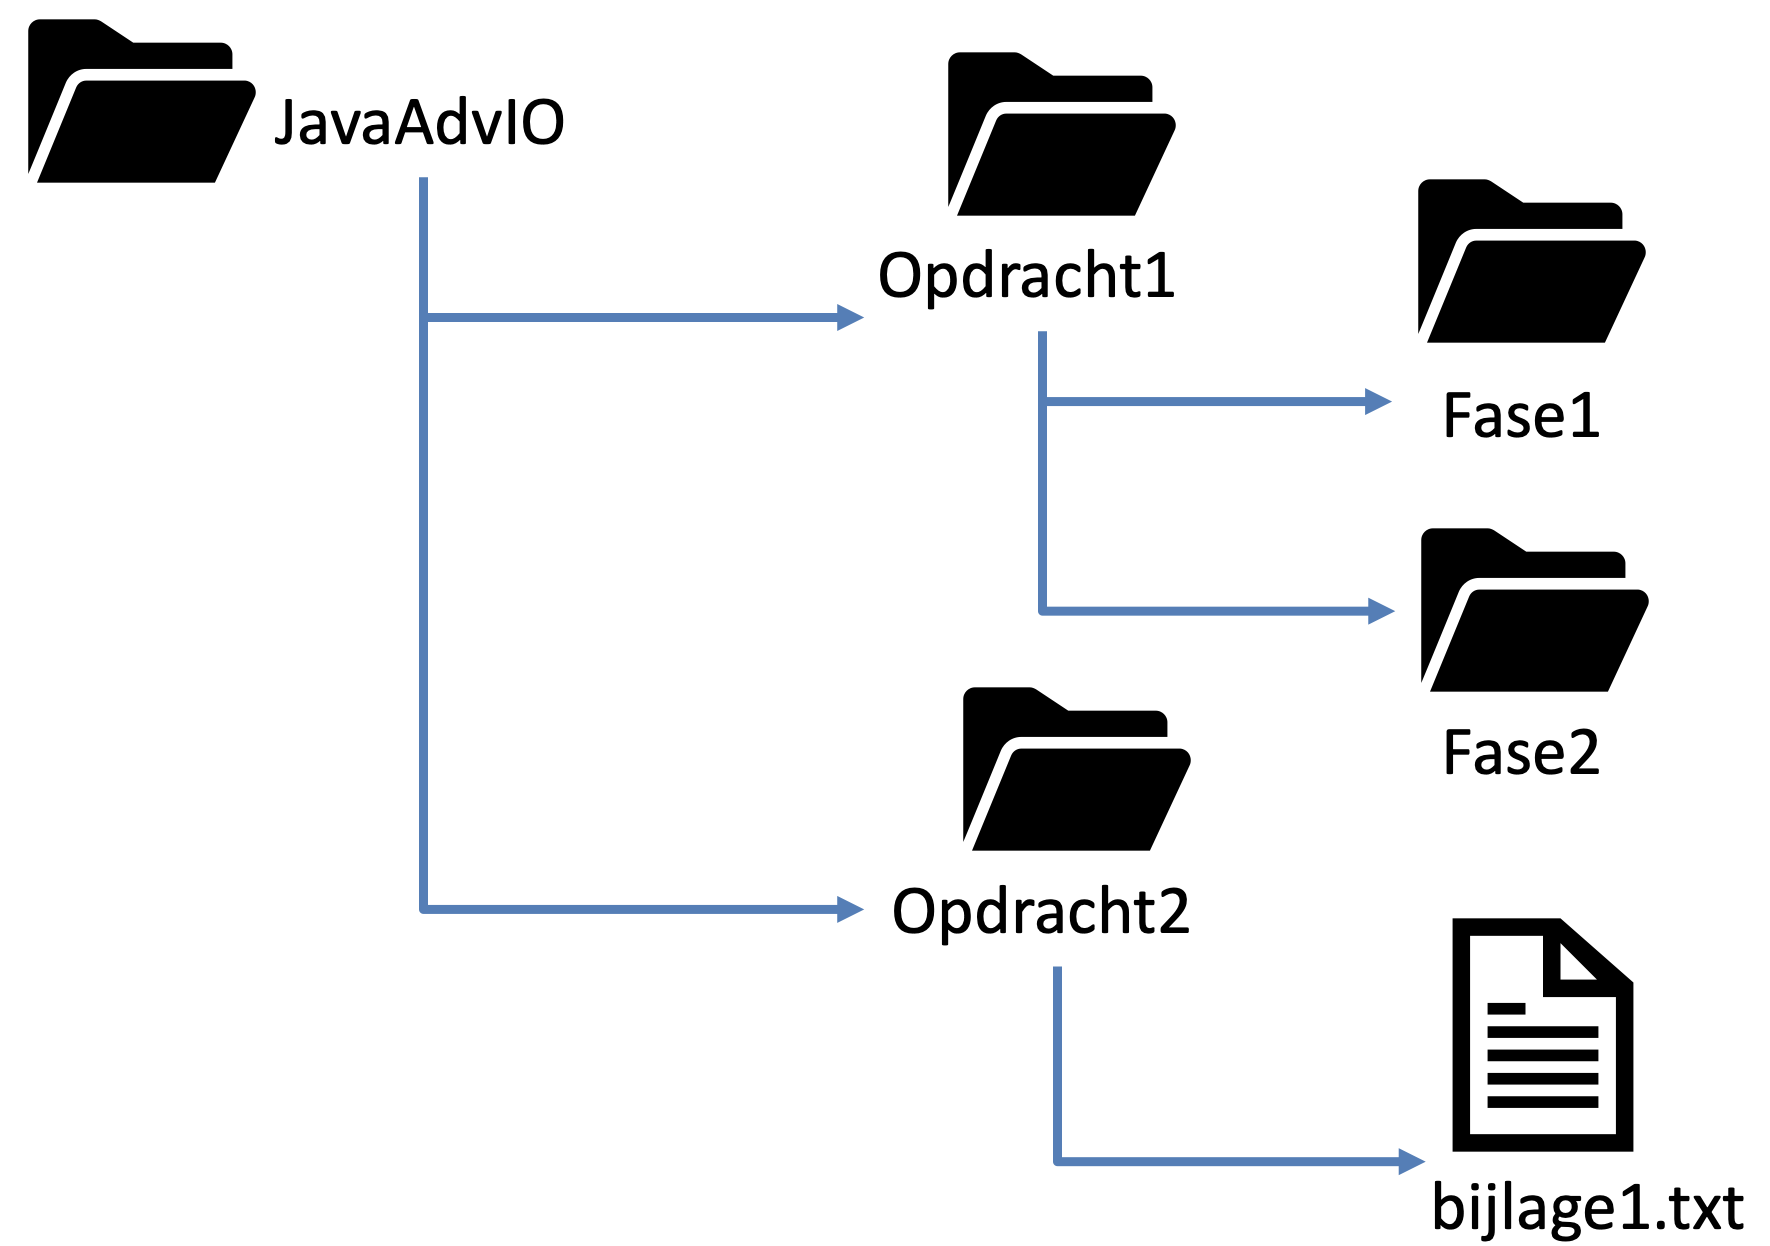
\includegraphics[width=\linewidth]{images/h8/opgave1.png}
  \caption{Bestandsstructuur}
  \label{fig:paths}
\end{figure}

\begin{itemize}
\item Vorm de systeemeigenschap user.home om tot een Path-object.
\item Welke concrete klasse heeft dit Path object?
\item Gebruik de methode resolve() van het Path object, om vanuit de directory user.home het path ``JavaAdvIO/Opdracht1/Fase2'' te volgen.
\item Wat is het resultaat wanneer je volgende methoden uitvoert op het laatst geconstrueerde Path?
\subitem toString()
\subitem getFileName()
\subitem getName(0)
\subitem getNameCount()
\subitem subpath(0,2)
\subitem getParent()
\subitem getRoot()
\end{itemize}
\end{oefening}




\subsection{De utility klasse Files}

De utility klasse \textit{java.nio.files.Files} bezit een groot aantal static methoden om bewerkingen met directories en bestanden uit te voeren.

\begin{oefening}
Zoek de documentatie van de klasse java.nio.files.Files op.
\end{oefening}

\subsubsection{Directories en bestanden aanmaken}

De static methode \textit{createDirectory} kan je gebruiken om een nieuwe directory aan te maken. 


\begin{lstlisting}
import java.io.IOException;
import java.nio.file.Files;
import java.nio.file.Path;

public class Demo03CreatingDirectoriesAndFiles {

	public static void main(String[] args) {
		Path path = Path.of(System.getProperty("user.home"), "JavaAdvIO", "Opdracht3", "bijlage.txt");
		if (Files.notExists(path.getParent())) {
			try {
				Files.createDirectory(path.getParent());
			} catch (IOException e) {
				System.out.println("An error occured while creating directory " + path.getParent());
			}
		}
		if (Files.notExists(path)) {
			try {
				Files.createFile(path);
			} catch (IOException e) {
				System.out.println("An error occured while creating file " + path);
			}
		}
	}

}
\end{lstlisting}

\begin{oefening}
Neem de documentatie er eens bij. Welke exceptions kunnen zich voordoen? Welke van deze exceptions zijn checked? Welke unchecked?
\end{oefening}


\subsubsection{Bestanden lezen (kleine bestanden)}

Als je tekstbestanden met een beperkt aantal regels wil lezen kan je de static methode readAllLines gebruiken.

\begin{lstlisting}
import java.nio.file.Path;
import java.nio.file.Paths;
import java.util.List;
import java.util.Random;

public class Demo04ReadingFiles {
	private static final Random RANDOM = new Random();

	public static void main(String[] args) {
		Path path = Paths.get("resources/small_file_with_text.txt");

		try {
			List<String> text = Files.readAllLines(path);
			System.out.println(text.get(RANDOM.nextInt(text.size())));
		} catch (IOException e) {
			e.printStackTrace();
		}
	}
}
\end{lstlisting}

\subsubsection{Bestanden kopi\"eren}

Je kan eenvoudig bestanden kopi\"eren door gebruik te maken van de static methode copy.

\begin{lstlisting}
import java.io.IOException;
import java.nio.file.Files;
import java.nio.file.Path;
import java.nio.file.Paths;

public class Demo05CopyFiles {

	public static void main(String[] args) {
		Path original = Paths.get("resources/small_file_with_text.txt");
		Path copy = Paths.get("resources", "copy_" + System.currentTimeMillis() + ".txt");
		System.out.println(Files.exists(copy));
		try {
			Files.copy(original, copy);
			System.out.println(Files.exists(copy));
		} catch (IOException e) {
			e.printStackTrace();
		}
	}
}
\end{lstlisting}

\section{Tekstbestanden}


A stream is an ordered sequence of bytes of an arbitrary length. Bytes flow over an output stream from an application to a destination and flow over an input stream from a source to an application.
The java.io package provides several output stream and input stream classes that are descendants of its abstract \textit{OutputStream} and \textit{InputStream} classes.



\begin{oefening}
Exercise: Image Processing in Java - Converting to Grayscale
Objective: Implement a Java program that simulates the process of receiving an image over a network, converting it to grayscale, and then preparing it for transmission. This exercise will help you understand how to manipulate images in memory using ByteArrayInputStream and ByteArrayOutputStream, along with the BufferedImage class for image processing tasks.

Background: In many applications, images need to be processed before they are stored or transmitted. Converting an image to grayscale is a common preprocessing step. In Java, this can be efficiently done using ByteArrayInputStream and ByteArrayOutputStream for in-memory data manipulation, along with BufferedImage for accessing and modifying image pixels.

Requirements:

Read an Image: Simulate receiving an image by loading it from the disk into a byte array. This step mimics downloading an image from the internet.
Convert to Grayscale: Use ByteArrayInputStream to read the byte array into a BufferedImage. Then, convert the image to grayscale by averaging the RGB values of each pixel.
Write the Processed Image: Use ByteArrayOutputStream to write the processed grayscale image to a byte array. This simulates preparing the image for uploading or further processing.
Instructions:

Setup: Start by reading an image file from disk and converting it to a byte array. This simulates receiving image data.
Processing:
Initialize a ByteArrayInputStream with the image byte array.
Use ImageIO.read to convert the byte stream into a BufferedImage.
Implement a method to convert the BufferedImage to grayscale. Iterate over each pixel, calculate the average of the red, green, and blue components, and set the new color for the pixel.
Output:
Initialize a ByteArrayOutputStream.
Use ImageIO.write to write the grayscale BufferedImage to the ByteArrayOutputStream.
You may convert the output stream back to a byte array if you wish to simulate sending the data over a network.
\end{oefening}



If you need to stream characters, you should take advantage of Java’s writer and reader classes, which were designed to support character I/O (they work with char instead of byte). Furthermore, the writer and reader classes take character encodings into account.



BufferedWriter and BufferedReader

BufferedWriter writes text to a character-output stream (a Writer instance), buffering characters so as to provide for the efficient writing of single characters, arrays, and strings. Invoke either of the following constructors to construct a buffered writer:

BufferedWriter(Writer out)
BufferedWriter(Writer out, int size)
The buffer size may be specified, or the default size (8,192 bytes) may be accepted. The default is large enough for most purposes.

BufferedWriter includes a handy void newLine() method for writing a line-separator string, which effectively terminates the current line.

BufferedReader reads text from a character-input stream (a Reader instance), buffering characters so as to provide for the efficient reading of characters, arrays, and lines. Invoke either of the following constructors to construct a buffered reader:

BufferedReader(Reader in)
BufferedReader(Reader in, int size)
The buffer size may be specified, or the default size (8,192 bytes) may be used. The default is large enough for most purposes.

\begin{oefening}

User Input:
Prompt the user to enter a secret message.
Ask for the number of positions to shift in the Caesar cipher (or any simple substitution cipher you choose to use).
Encoding the Message:
Apply the cipher to the message, shifting each letter by the specified number of positions.
Charset Conversion:
Write the encoded message to a file using a specified source charset.
Read the file and convert the charset to a different one, simulating sending the message through a different system.
Decoding the Message:
After converting it back to the original charset, decode the message by reversing the cipher.
Display:
Show the original, encoded, and decoded messages to the user, highlighting how the message remains confidential and intact through the encoding and charset conversion process.

\end{oefening}

\subsection{I/O Streams}

Een I/O stream is een opeenvolging van bytes (8 bits). Je mag I/O streams zeker niet verwarren met de Stream API die we in het vorige hoofdstuk hebben besproken. InputStreams worden gebruikt om gegevens byte per byte aan te bieden aan een Java programma. OutputStreams worden gebruikt om gegevens vanuit een Java programma byte per byte te versturen naar een externe bron (dit kan een bestand zijn, maar ook een andere computer). 
In dit hoofdstuk zijn het bestanden die we als bron of doel van onze I/O streams gebruiken. Je kan tekstbestanden byte per byte gaan inlezen en wegschrijven, maar dit is niet effici\"ent. Karakters worden meestal voorgesteld door meerdere bytes. 
De karakter encodering bepaalt hoeveel bytes er per karakter gebruikt zullen worden. Bij UTF-8 bijvoorbeeld worden 1 tot 4 bytes gebruikt om de karakters voor te stellen. Een alternatief is dus dat je tekstbestanden karakter per karakter gaat inlezen, maar ook dit is niet altiijd effici\"ent.

\subsection{BufferedReader}

De klasse BufferedReader biedt een eenvoudige en effici\"ente manier om grotere tekstbestanden te lezen. Het groepeert (buffert) karakters uit een bestand zodat je het bestand regel per regel kan inlezen. De methode newBufferedReader uit de klasse Files vereenvoudigt het aanmaken van de BufferedReader voor ons.
Het einde van het tekstbestand is bereikt als readLine() \textit{null} geeft.

\begin{figure}[H]
  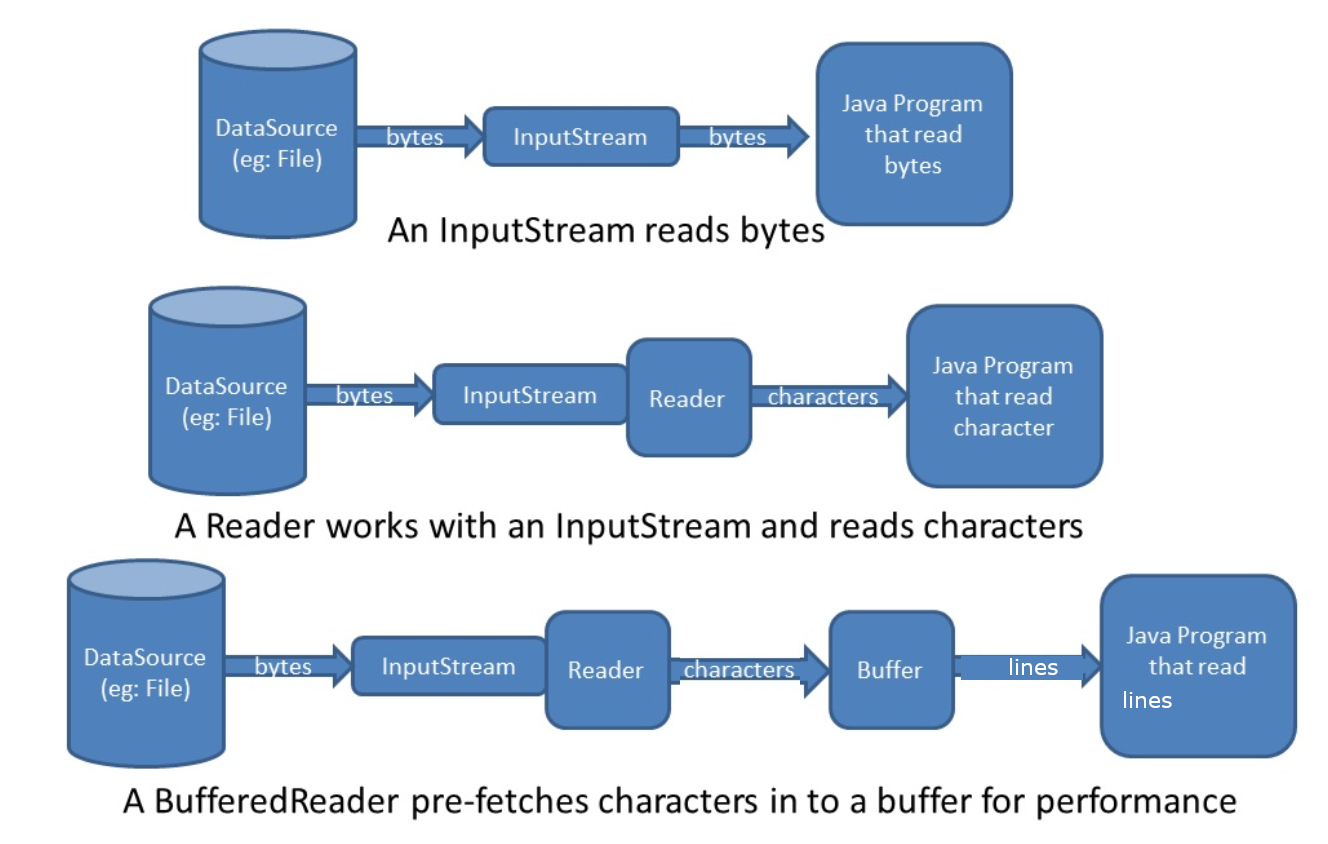
\includegraphics[width=\linewidth]{images/h8/stream_reader.png}
  \caption{InputStream, InputStreamReader en BufferedReader}
  \label{fig:paths}
\end{figure}

\begin{lstlisting}
import java.io.BufferedReader;
import java.io.IOException;
import java.nio.file.Files;
import java.nio.file.Paths;

public class Demo06BufferedReader {

	public static void main(String[] args) {

		try (BufferedReader reader =  Files.newBufferedReader(Paths.get("resources/small_file_with_text.txt"))) {
			String line = null;
			while ((line = reader.readLine()) != null) {
				System.out.println(line);
			}
		} catch (IOException e) {
			e.printStackTrace();
		}
	}
}
\end{lstlisting}

We maken in dit code-voorbeeld gebruik van \textbf{try-with-resources}.
De BufferedReader implementeert namelijk de interface \textit{java.lang.AutoCloseable}. Wanneer je klaar ben met het lezen of schrijven van een bestand, moet je dit namelijk aan het besturingssysteem laten weten. Het besturingssyteem zorgt ervoor dat de toegang tot een bestand goed beheerd wordt zodat er zich geen problemen voordoen wanneer er verschillende programma's gelijktijdig in hetzelfde bestand willen lezen en/of schrijven. Het sluiten van een bestand werd typisch ge\"implementeerd in een \textit{finally-block}. Tegenwoordig zijn veel resources (zoals bestanden) auto-closeable waardoor je deze code niet meer zelf moet schrijven. Door gebruik te maken van try-with-resources wordt het bestand automatisch netjes gesloten zodra het programma klaar is met het lezen of schrijven van het bestand.

\subsection{BufferedWriter}

In plaats van karakter per karakter in een bestand weg te schrijven, gaat BufferedWriter grotere stukken tekst in \'e\'en keer in het bestand wegschrijven. 




\subsection{Character sets}

\begin{lstlisting}
import java.nio.charset.Charset;

public class Demo7DefaultCharset {

	public static void main(String[] args) {

		System.out.println(Charset.defaultCharset().displayName());
	}

}
\end{lstlisting}

Met het bovenstaande programma kan je afdrukken wat de default encoding is die gebruikt wordt om bytes te combineren tot karakters. UTF-8 is de meest gebruikte encoding, maar toch is het een goede gewoonte om de gebruikte karakterset mee te geven als parameter wanneer je een bestand leest of schrijft. Op die manier kan je problemen vermijden.

\begin{lstlisting}
Files.newBufferedWriter(Paths.get("resources/myfile.txt"), Charset.forName("UTF-8"));
\end{lstlisting}


\begin{oefening}
Find out what words are shared by two files, and return the
number of unique words in common. Output the words you find to
a different file.
1 long wordsInCommon ( File file1 , File file2 ) {
2 // TODO implement
3 }

\end{oefening}

\subsection{Het decorator patroon}

De BufferedReader heeft als basis een InputStreamReader waaraan extra functionaliteit wordt toegevoegd, namelijk het bufferen van de karakters. De InputStreamReader vormt op zijn beurt de brug tussen byte streams en character streams. Hij leest bytes en decodeert ze tot karakters door gebruik te maken van een karakterset (Charset).

Wat we bij deze klassen is dat ze ontwikkeld zijn volgens het decorator ontwerppatroon.
In het package \textit{be.pxl.ja.decorator} vind je een eenvoudig voorbeeld van dit ontwerppatroon.

\section{Programma attributen}

Het is een goed idee om Java programma's gemakkelijk configureerbaar te maken. 
Om dit te verwezenlijken zijn parameters bestaande uit een key en een value meestal voldoende. 
In Java gebruik je de klasse \textit{java.util.Properties} om configuratie-bestanden te lezen en weg te schrijven.
Je gebruikt de methode load om een configuratie-bestand in te lezen en store om de eigenschappen weg te schrijven. Met de methode getProperty kan je aan de hand van een key de bijhorende waarde opvragen.

\begin{lstlisting}
import java.io.IOException;
import java.io.InputStream;
import java.io.OutputStream;
import java.nio.file.Files;
import java.nio.file.Path;
import java.util.Properties;
import java.util.Scanner;

public class Demo08ProgramWithProperties {
	private static final String CONFIG_FILE = "resources/config.properties";

	public static void main(String[] args) {
		try(InputStream inputStream = Files.newInputStream(Path.of(CONFIG_FILE))) {
			Properties properties = new Properties();
			properties.load(inputStream);
			System.out.println("Welcome " + properties.getProperty("demo.name") + "!");
			System.out.println("You're mails will be sent to: " + properties.getProperty("demo.email"));
		} catch (IOException e) {
			createProperties();
		}
	}

	private static void createProperties() {
		Scanner scanner = new Scanner(System.in);
		System.out.println("You're using this program for the first time.");
		System.out.println("What's your name:");
		String name = scanner.nextLine();
		System.out.println("What's your company:");
		String company = scanner.nextLine();
		System.out.println("What's your email:");
		String email = scanner.nextLine();
		Properties properties = new Properties();
		properties.setProperty("demo.name", name);
		properties.setProperty("demo.company", company);
		properties.setProperty("demo.email", email);
		try(OutputStream outputStream = Files.newOutputStream(Path.of(CONFIG_FILE))) {
			properties.store(outputStream, "Demo program configuration");
		}
		catch (IOException e) {
			System.out.println("We were not able to save your configuration.");
		}
	}
}
\end{lstlisting}

De eerste keer dat het programma wordt uitgevoerd, is het bestand config.properties bestand nog niet aanwezig is. De gebruiker wordt dan gevraagd om zijn gegevens in te voeren.

\begin{verbatim}
You're using this program for the first time.
What's your name:
Nele
What's your company:
PXL
What's your email:
nele.custers@pxl.be
\end{verbatim}

Je zal zien dat er na het uitvoeren van het programma een bestand \textit{resources/config.properties} is aangemaakt.
Dit bestand bevat de volgende informatie.

\begin{verbatim}
#Demo program configuration
#Tue Nov 17 09:13:51 CET 2020
demo.name=Nele
demo.company=PXL
demo.email=nele.custers@pxl.be
\end{verbatim}
Wanneer je het programma opnieuw opstart, wordt het .properties bestand gelezen en krijg je de volgende output.

\begin{verbatim}
Welcome Nele!
You're mails will be sent to: nele.custers@pxl.be
\end{verbatim}


\section{Byte stream}

Object serialization laat ons toe om de status (de waarden van de eigenschappen) van een object te converteren naar een byte stream. Op die manier kan een object weggeschreven worden in bestand of verstuurd worden over een netwerk.
Deserialization is het omgekeerde proces, waarbij de byte stream terug wordt geconverteerd naar een object.

Enkel objecten van klassen die de interface \textit{Serializable} implementeren kunnen geserialiseerd worden.
Je kan een eigenschap van een klasse \textbf{transient} maken als je de waarde van die eigenschap niet wil serialiseren.

Alle static eigenschappen behoren tot de klasse en niet tot een object, dus de waarden van static field kunnen nooit geserialiseerd worden. 

De klasse ObjectOutputStream die we gebruiken om objecten te schrijven en de klasse ObjectInputStream die we gebruiken om objecten in te lezen, zijn opnieuw implementaties van het decorator patroon. We gaan respectievelijk de klassen FileOutputStream en FileInputStream ``decoreren'' met extra functionaliteit om te werken met volledige objecten in plaats van bytes. 

\subsection{Object serialization}

\begin{lstlisting}
import java.io.FileOutputStream;
import java.io.IOException;
import java.io.ObjectOutputStream;
import java.time.LocalDate;
import java.util.Arrays;
import java.util.List;

public class Demo09Serialization {

	public static void main(String[] args) {
		Student student = new Student("Mare", LocalDate.of(2000, 11, 29));
		student.setGraduationDate(LocalDate.of(2018, 6, 30));
		List<String> animals = Arrays.asList("elephant", "zebra", "donkey");
		try (FileOutputStream file = new FileOutputStream("resources/demo.ser");
		     ObjectOutputStream out = new ObjectOutputStream(file)) {
			out.writeObject(student);
			out.writeObject(animals);
		} catch (IOException ex) {
			System.out.println(ex.getMessage());
		}
	}
}
\end{lstlisting}


\subsection{Object deserialization}

\begin{lstlisting}
import java.io.FileInputStream;
import java.io.IOException;
import java.io.ObjectInputStream;
import java.util.List;

public class Demo09Deserialization {

	public static void main(String[] args) {
		try (FileInputStream file = new FileInputStream("resources/demo.ser");
		     ObjectInputStream in = new ObjectInputStream(file)) {
			Student student = (Student) in.readObject();
			System.out.println(student.getName());
			System.out.println(student.getDateOfBirth());
			List<?> animals = (List<?>) in.readObject();
			//List<String> animals = (List<String>) in.readObject();
			System.out.println(animals.size());
			System.out.println(animals.get(0));
		} catch (IOException ex) {
			System.out.println(ex.getMessage());
		} catch (ClassNotFoundException e) {
			e.printStackTrace();
		}
	}
}
\end{lstlisting}


%\subsection{Audio en afbeeldingen}



\section{Oefeningen}

\begin{oefening}
\textbf{Telefoonboek}\\

Schrijf een programma om telefoonnummers bij te houden.
Wanneer je het programma opstart wordt het bestand phonedirectory.txt ingelezen,
plaats dit dus in een nieuwe folder (bv. resources) in je project. Iedere lijn in het
bestand heeft het volgende formaat: $<naam>;<tel1>;<tel2>;…$
We geven alvast wat startcode voor het printen van het menu.
(PhoneNumbersApp.java)
\begin{itemize}
\item Lees alle lijnen in en steek alle contacten in een Collection, zodat je aan de hand van
een naam de bijhorende telefoonnummers kan zoeken. Let op: er kunnen meerdere
telefoonnummers aan één contact gelinkt worden.
\item Zorg ook voor functionaliteit om telefoongegevens toe te voegen (zie reeds gegeven
code). Als je een telefoonnummer toevoegt dat reeds bestaat voor de gegeven
persoon, gooit het programma een zelfgemaakte exception. (bv.
PhoneDirectoryException). Deze exception moet niet opgevangen worden, dus het
programma mag stoppen met uitvoeren in dit geval.
\item Wanneer je ervoor kiest om het programma af te sluiten, worden alle gegevens eerst
weer weggeschreven in phonedirectory.txt, zodat geen gegevens verloren gaan.
\end{itemize}
\end{oefening}

\begin{oefening}
\textbf{Bank account}\\

Schrijf een applicatie voor het beheren van spaarrekeningen.
Voorzie volgende functionaliteit:
\begin{itemize}
\item Maak een klasse Spaarrekening met de nodige member variabelen (bv. saldo,
naam, nummer, …)
\item Zorg dat instanties van deze klasse als object naar een file geschreven kunnen
worden (Serializable interface)
\item Schrijf in een main methode de code om een volledig Spaarrekening object
naar een file weg te schrijven.
\item Voeg code toe om een spaarrekening object terug uit te lezen uit deze file.
\item Controleer of de member variabelen hun waarde hebben behouden na uitlezen.
\end{itemize}
\end{oefening}


\section{Spring Boot File Handling}





\section{outline}

 Reading and Writing Files
Streams: Introduce InputStream and OutputStream for reading from and writing to byte streams (e.g., FileInputStream, FileOutputStream).
Readers and Writers: Discuss Reader and Writer for character stream operations (e.g., FileReader, FileWriter).
Buffering: Explain the use of BufferedReader and BufferedWriter for efficient reading and writing.
3. Working with Directories
Directory Operations: Methods for listing files in a directory, creating directories, etc.
4. Advanced File Operations
Random Access File: Usage of RandomAccessFile class for reading and writing to any location in a file.
5. Java NIO Package
Path and Paths: Introduce Path class as an upgrade to java.io.File.
Files Class: Utilizing Files class for file operations like checking, deleting, copying, moving files, reading, and writing.
File Channels: Discuss FileChannel for reading, writing, mapping, and manipulating a file.
Buffers and ByteBuffers: Understanding how data is buffered in NIO.
Asynchronous File I/O: Introduce AsynchronousFileChannel for asynchronous file operations.
6. Exception Handling in File I/O
Try-with-resources: Best practices for handling exceptions and ensuring that files are properly closed using the try-with-resources statement.
Handling IOExceptions: Strategies for handling IOException.
7. Serialization and Deserialization
Object Streams: Using ObjectInputStream and ObjectOutputStream for object serialization.
8. Practical Exercises and Examples
File Copy: Implement a program to copy a file.
File Browser: Create a simple console-based or GUI file browser.
Text File Processing: Read a text file, process its content, and write the output to another file.
9. Best Practices
File Handling Best Practices: Discuss best practices in file handling such as closing resources, handling exceptions, and ensuring efficient data processing.


Here are some best practices for reading and writing to files using Java libraries:

Use try-with-resources: When reading or writing to a file, it’s important to properly handle the opening and closing of the file stream. Java 7 introduced the try-with-resources statement which automatically closes the file stream once the code block is executed.
Use buffered streams: Reading or writing large files can be a performance bottleneck. Using buffered streams can help improve performance by reducing the number of I/O operations required.
Handle exceptions: When reading or writing to a file, it’s important to handle any exceptions that may occur. Common exceptions include FileNotFoundException and IOException.
Use appropriate encoding: When reading or writing text files, it’s important to use the appropriate encoding. The default encoding used by Java is usually UTF-8, but this may not be appropriate for all scenarios.
Use relative paths: When working with files, it’s best to use relative paths instead of absolute paths. This makes the code more portable and easier to maintain.
Check for file existence: Before reading or writing to a file, it’s important to check if the file exists. This can be done using the File.exists() method.
Use descriptive file names: When creating new files, it’s important to use descriptive file names that are easy to understand and maintain. This can help prevent naming conflicts and make it easier to find and manage files.
Use constants for file paths: When working with file paths, it’s best to use constants instead of hardcoding the paths in the code. This makes it easier to update file paths in the future.
Close file streams: When finished with a file, it’s important to close the file stream to free up system resources. This can be done using the close() method.
Handle file locking: When working with files, it’s important to handle file locking to prevent multiple processes from accessing the same file at the same time. Java provides a number of methods for handling file locking, including the FileChannel.lock() method.
10. Recent Developments and Additional Resources
Updates in Latest Java Versions: Briefly cover any recent changes or enhancements in file handling in newer Java versions.
External Libraries: Introduction to popular third-party libraries for file handling, if time allows.



\chapter{To define}


Upload a file and generate a pdf in with spring boot....

code quality with sonarqube


\section{Exercise}

In the exercise we implement a REST endpoint that returns a PDF file.

\begin{lstlisting}
@GetMapping(value = "/pdfreport", produces = MediaType.APPLICATION_PDF_VALUE)
public @ResponseBody byte[] createPdfReport() {

    ByteArrayInputStream bis = GeneratePdfReport.createReport();

	return bis.readAllBytes();
}
\end{lstlisting}

In the example above we assume to have a helper class GeneratePdfReport that has a method returning a ByteArrayInputStream with the data of your PDF file. We use the @ResponseBody annotation on the controller method to indicate that the object returned by the method should be marshaled directly to the HTTP response body.

For creating PDF files in Java, we'll use itextpdf: \url{https://mvnrepository.com/artifact/com.itextpdf/itextpdf}.

For creating the qr code we will use the ZXing (`Zebra Crossing') API, a popular API for QR code processing in Java. You'll need to include 2 artifacts to be able to generate QR codes.

\begin{lstlisting}
<dependency>
	<groupId>com.google.zxing</groupId>
	<artifactId>core</artifactId>
	<version>3.4.0</version>
</dependency>
<dependency>
	<groupId>com.google.zxing</groupId>
	<artifactId>javase</artifactId>
	<version>3.4.0</version>
</dependency>
\end{lstlisting}

Here is the full code for filling the name and QR code in the PDF template.

\begin{lstlisting}
package be.pxl.superhero.service.impl;

import be.pxl.superhero.api.SuperheroDTO;
import be.pxl.superhero.commons.Cipher;
import com.google.zxing.BarcodeFormat;
import com.google.zxing.WriterException;
import com.google.zxing.client.j2se.MatrixToImageWriter;
import com.google.zxing.common.BitMatrix;
import com.google.zxing.qrcode.QRCodeWriter;
import com.itextpdf.text.DocumentException;
import com.itextpdf.text.Element;
import com.itextpdf.text.Image;
import com.itextpdf.text.Phrase;
import com.itextpdf.text.pdf.ColumnText;
import com.itextpdf.text.pdf.PdfContentByte;
import com.itextpdf.text.pdf.PdfReader;
import com.itextpdf.text.pdf.PdfStamper;
import org.springframework.stereotype.Component;

import java.io.ByteArrayInputStream;
import java.io.ByteArrayOutputStream;
import java.io.IOException;
import java.net.URISyntaxException;
import java.nio.file.Path;
import java.nio.file.Paths;

@Component
public class SuperheroIdCardGenerator {

    public ByteArrayInputStream superheroIdCard(SuperheroDTO superhero) {

        ByteArrayOutputStream out = new ByteArrayOutputStream();

        try {
            Path path = 
                Paths.get(ClassLoader.getSystemResource("superheroidcard.pdf").toURI());
            PdfReader pdfReader = new PdfReader(path.toUri().toURL());
            PdfStamper pdfStamper = new PdfStamper(pdfReader, out);
            PdfContentByte canvas = pdfStamper.getOverContent(1);
            ColumnText.showTextAligned(canvas, Element.ALIGN_LEFT, new Phrase(superhero.firstName() + " " + superhero.lastName()), 200, 620, 0);
            ColumnText.showTextAligned(canvas, Element.ALIGN_LEFT, new Phrase(superhero.superheroName()), 200, 550, 0);
            byte[] qrCodeImage = getQRCodeImage(Cipher.skipALetter(superhero.superheroName()), 130, 130);
            Image qrCode = Image.getInstance(qrCodeImage);
            qrCode.setAbsolutePosition(190, 360);
            canvas.addImage(qrCode);
            pdfStamper.close();
            pdfReader.close();
        } catch (DocumentException | URISyntaxException | IOException | WriterException ex) {
            // TODO: add logging - see next chapter
            throw new PdfCreationException(ex);
        }
        return new ByteArrayInputStream(out.toByteArray());
    }

    public static byte[] getQRCodeImage(String text, int width, int height) throws WriterException, IOException {
        QRCodeWriter qrCodeWriter = new QRCodeWriter();
        BitMatrix bitMatrix = qrCodeWriter.encode(text, BarcodeFormat.QR_CODE, width, height);

        ByteArrayOutputStream pngOutputStream = new ByteArrayOutputStream();

        MatrixToImageWriter.writeToStream(bitMatrix, "PNG", pngOutputStream);
        return pngOutputStream.toByteArray();
    }
}
\end{lstlisting}

The PdfReader first opens the PDF template file. The PdfStamper is used for adding the full name, the alias and the
QR code (as an image) to the template. The newly generated PDF is returned as a ByteArrayInputStream.

\begin{oefening}

All superheroes need an id card. Your job as a developer is to create a REST endpoint where we can download a pdf with the id card.

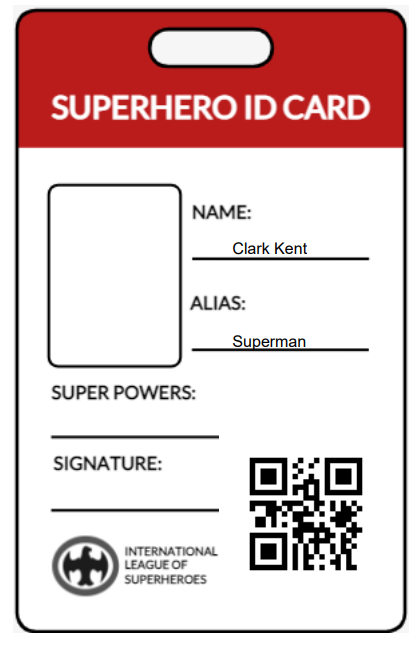
\includegraphics[width=5cm]{./images/chapter3/superhero_id_card.png}

The pdf template can be found in blackboard. 

$\square$ Download the pdf template and add it to the resources directory of your superhero-backend project.

\vspace{5mm}

We will include the full name, the superhero name and a unique QR code in the template.
The generated pdf will be available at the endpoint:
\url{http://localhost:<port>/api/superheroes/<superheroId>/idcard}

The QR code will contain the scrambled alias of a superhero. 

\vspace{5mm}

$\square$ Create the utility class Cipher with a static method skipALetter which takes a String as a parameter and returns the scrambled String. To encrypt a sentence you divide each word into half. If a word has an odd number of letters, the first group of letters contains one letter extra. Take the first letter of the first group, followed by the first letter of the second group. Then, write the second letter of the first group and the second letter of the second group, and so on, until all the words are encrypted. For example, if your sentence is `SECRET CODES', it will be encrypted as `SREECT CEOSD'.

Write unit tests to test your implementation. 
\begin{itemize}
\item unit test for one word with even length
\item unit test for one word with odd length
\item unit test for a sentence with multiple words with odd and even length
\item unit test for an empty string (should return an empty string)
\end{itemize}

\vspace{5mm}

$\square$ Implement the REST endpoint for retrieving a superhero's id card.  
\end{oefening}

\section{Code quality with SonarQube}

We would like to deliver high quality Java code. SonarQube is a Java analyzer that checks the quality of our code and detects code smells.

\begin{oefening}

Create a docker container with SonarQube. Run the following command in a terminal window:

\fbox{\strut docker run -d -{}-name sonarqube -p 9000:9000 -p 9092:9092 sonarqube}

Open \url{http://localhost:9000} in a browser. You can login with the default username `admin' and password `admin'. Next you have to update the default password (you have to choose a new password!).

\vspace{5mm}

Create a new SonarQube project for the superhero-backend application. Click on the button `Manually', fill out the project details and choose to analyze your project locally. A token will be generated.

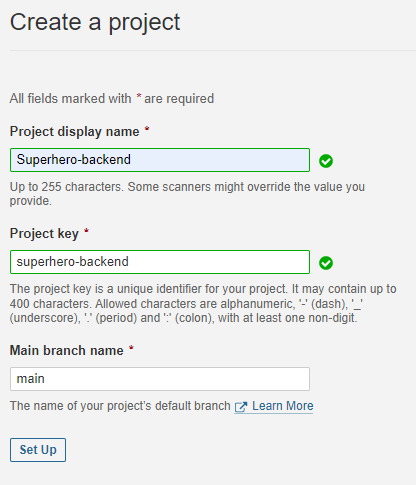
\includegraphics{./images/chapter3/sonarqube_create_project.png}

Now we can update the pom.xml file of our superhero-backend to run the code analysis.

First we need a sonar profile to provide the url, project key and token.

\begin{lstlisting}
<profiles>
	<profile>
		<id>sonar</id>
		<activation>
			<activeByDefault>true</activeByDefault>
		</activation>
		<properties>
			<sonar.host.url>http://localhost:9000</sonar.host.url>
			<sonar.projectKey>superhero-backend</sonar.projectKey>
			<sonar.login>sqp_6319ae2795ccdc24baa3a994962a8bbaa0b0cc16</sonar.login>
		</properties>
	</profile>
</profiles>
\end{lstlisting}

Run the following maven command to perform the code analysis:
\fbox{\strut \$mvn clean verify sonar:sonar}

\vspace{5mm}

Open the SonarQube dashboard \url{http://localhost:9000/dashboard?id=superhero-backend} to get an overview of possible bugs, vulnerabilities and code smells.
You can get a more in-depth explanation of the code quality rules including examples at \url{https://rules.sonarsource.com/java}. Namely, \url{https://rules.sonarsource.com/java/RSPEC-5786} is an interesting code smell to look at.

\vspace{5mm}

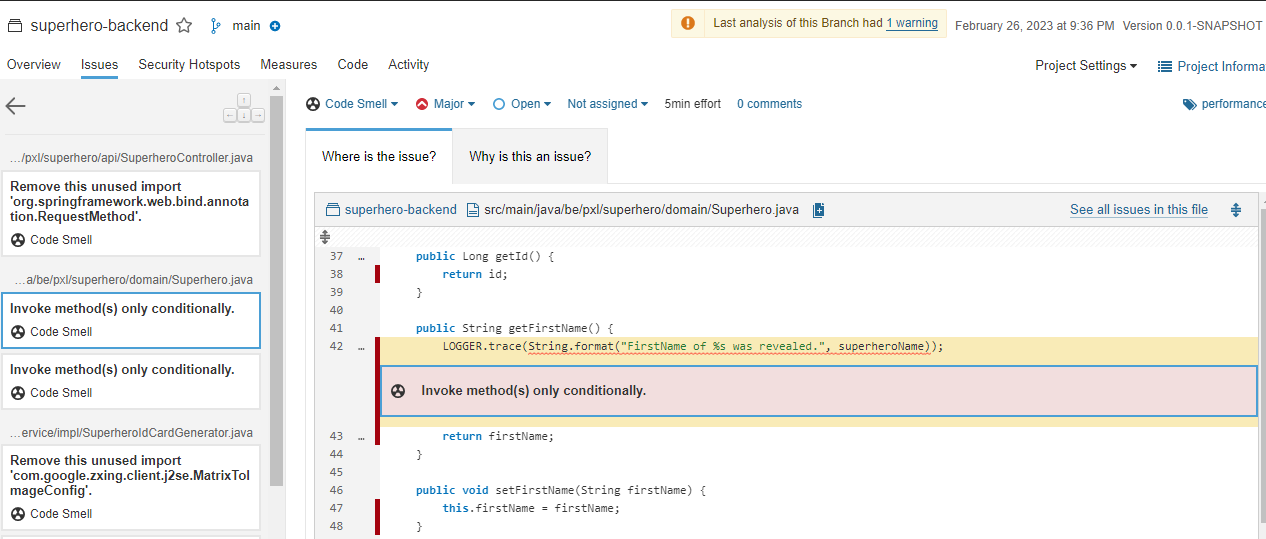
\includegraphics[width=\textwidth]{./images/chapter3/sonarqube.png}

When you look at the dashboard, you'll see the code coverage is always 0.0\%. JaCoCo is needed to generate an extra report to display the code coverage.

First add the property jacoco.version in the pom.xml file:

\begin{lstlisting}
<properties>
	<java.version>17</java.version>
	<jacoco.version>0.8.7</jacoco.version>
</properties>
\end{lstlisting}

Next, add the JaCoCo maven plugin to your project.

\begin{lstlisting}
<build>
	<plugins>
		<plugin>
			<groupId>org.jacoco</groupId>
			<artifactId>jacoco-maven-plugin</artifactId>
			<version>${jacoco.version}</version>
			<executions>
				<execution>
					<id>prepare-agent</id>
					<goals>
						<goal>prepare-agent</goal>
					</goals>
				</execution>
				<execution>
					<id>report</id>
					<phase>test</phase>
					<goals>
						<goal>report</goal>
					</goals>
				</execution>
			</executions>
		</plugin>
	</plugins>
	<pluginManagement>
		<plugins>
			...
		</plugins>
	</pluginManagement>
</build>
\end{lstlisting}

During the test phase JaCoCo will generate a report and save it in the directory target/site/jacoco/jacoco.xml. SonarQube will automatically check this location and the report will be picked up.
First remove the empty, automatically created Spring Boot test from your test folder.
Run the Maven command again and check your code coverage.

\end{oefening}

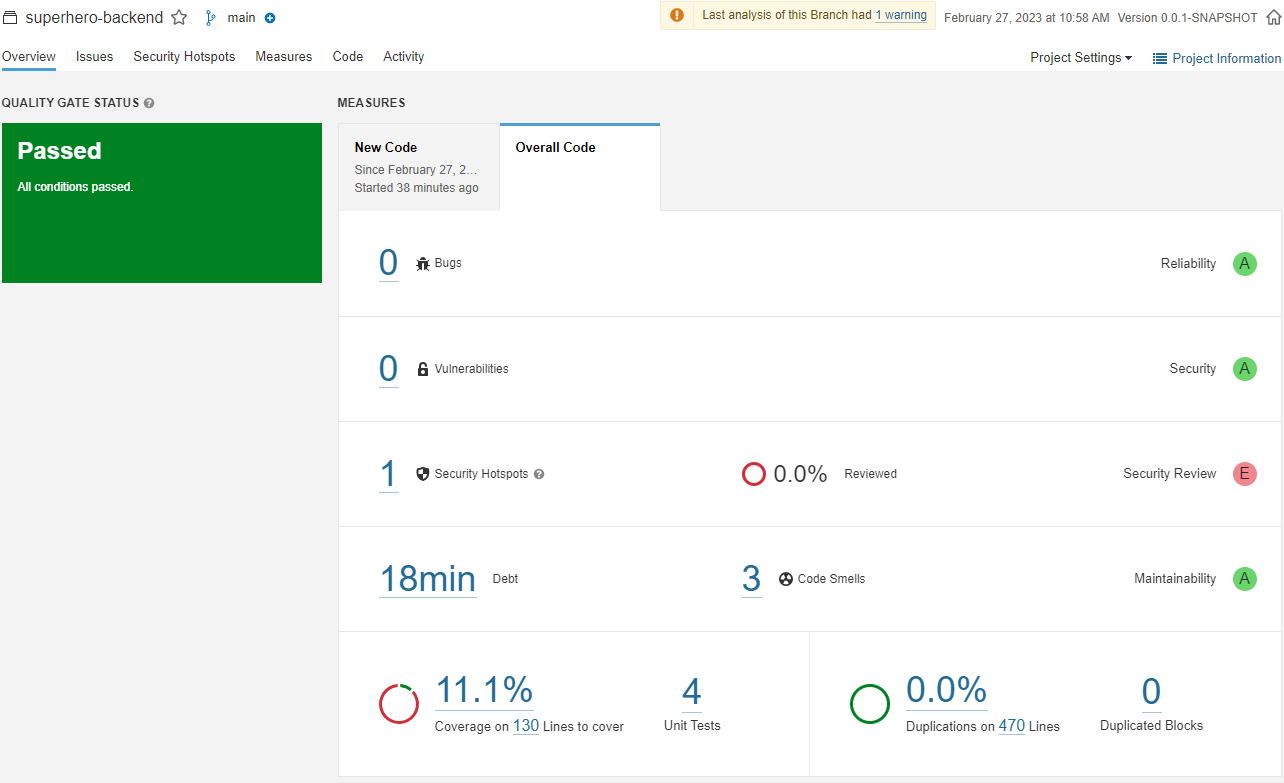
\includegraphics[width=\textwidth]{./images/chapter3/sonarqube-report.png}

A good application of priority queues is finding the shortest path in a graph. A common algorithm for this is Dijkstra’s algorithm.

https://textbooks.cs.ksu.edu/cc315/iv-priority-queues/10-heaps-and-priority-queues/5-dijkstras/
\chapter{Code quality}




\chapter{Introduction}
    
\fcolorbox{black}[HTML]{E9F0E9}{\parbox{\textwidth}{%
\noindent \textbf{Learning goals}\\
The junior-colleague
\begin{enumerate}[nolistsep]
\item can describe what Spring is
\item can describe what Spring Boot is
\item can explain what a three-tier application is
\item can identify the three layers in a Spring Boot application
\item can explain the responsibilities of the layers in a Spring Boot application
\item can explain the architecture of a Spring RESTful web application
\item can explain what a DTO is
\item can explain what an entity-object is
\item can explain what dependency injection is
\item can explain what a Spring bean is
\item can explain what a Spring container is
\item can explain what a Spring Boot starter is
\end{enumerate}}}


\section{Enterprise Applications with Java}
By 1999, Java had developed a loyal following among application developers and Sun saw an opportunity to extend the language for traditional enterprise workloads. With the launch of J2EE, and another technology that was gaining prominence — the application server — enterprises now had a platform that was designed to meet their needs with capabilities for things like security, scalability and reliability.

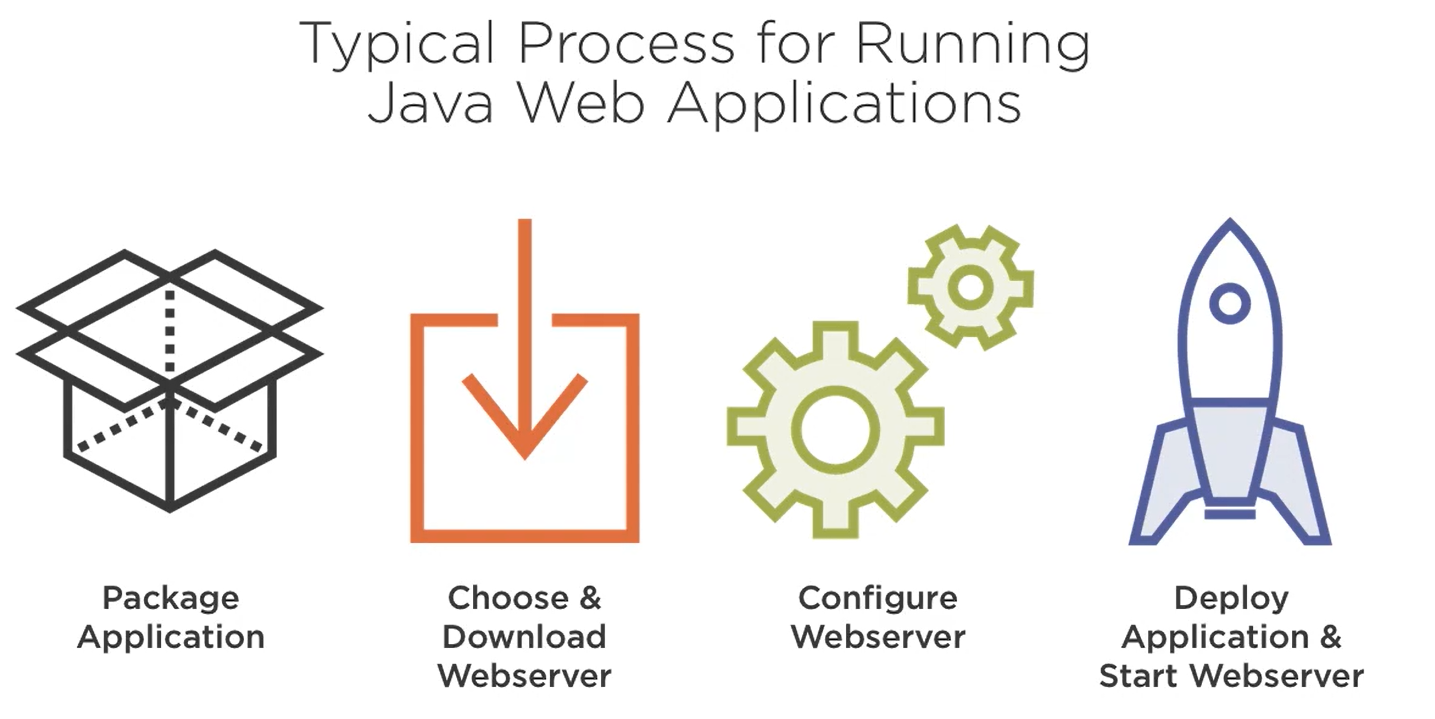
\includegraphics[width=\textwidth]{./images/chapter1/before_spring_boot.png} 

Spring came into being in 2003 as a response to the complexity of the early J2EE specifications. While some consider Java EE and its modern-day successor Jakarta EE to be in competition with Spring, they are in fact complementary. The Spring programming model does not embrace the Jakarta EE platform specification; rather, it integrates with carefully selected individual specifications from the traditional EE umbrella. Spring started as a lightweight alternative to Java Enterprise Edition. Rather than develop components as heavyweight Enterprise
JavaBeans (EJBs), Spring offered a simpler approach to enterprise Java development, utilizing dependency injection and aspect-oriented programming to achieve the capabilities of EJB with plain old Java objects (POJOs).
But while Spring was lightweight in terms of component code, it was heavyweight in terms of configuration. Initially, Spring was configured with XML (and lots of it).
It provides everything you need to create Java enterprise applications. Spring offers the flexibility to create many kinds of architectures depending on an application’s needs. As of Spring Framework 6.0, Spring requires Java 17+.

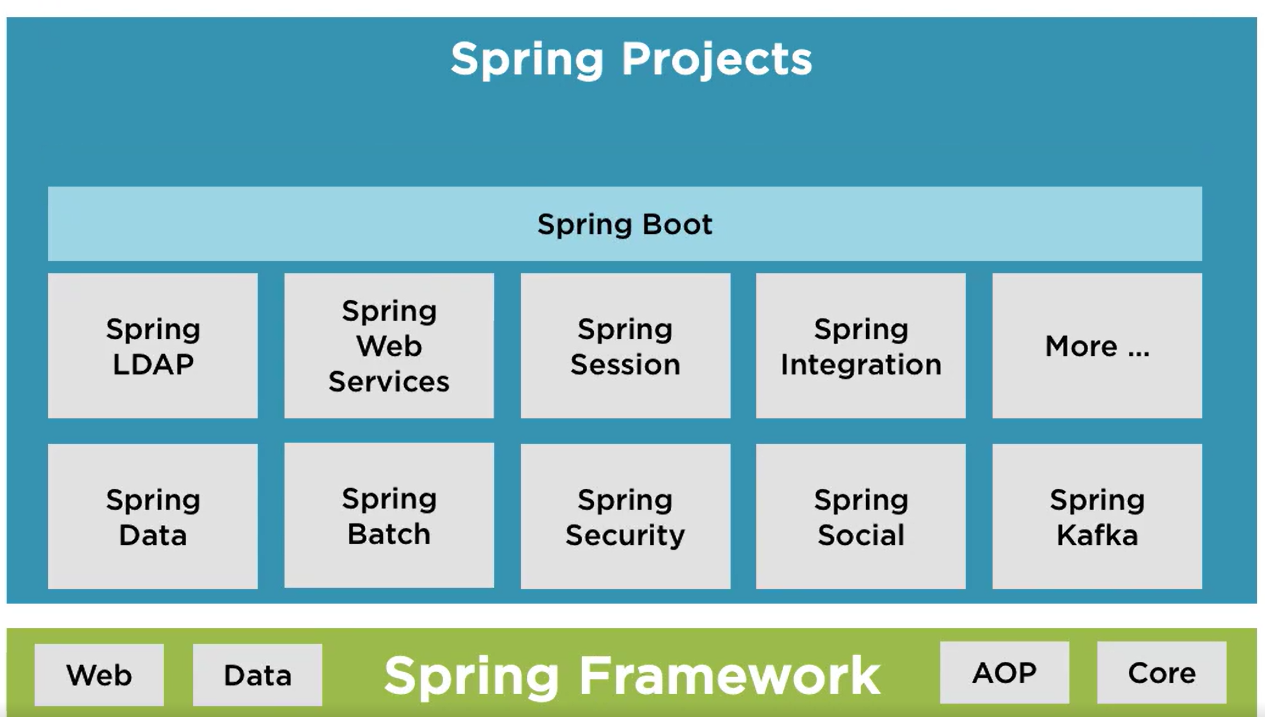
\includegraphics[width=\textwidth]{./images/chapter1/spring_framework.png} 

Spring Boot is a project that is built on the top of the Spring Framework. It provides an easier and faster way to set up, configure, and run java applications.

    
\section{What is Spring Boot?}
 
Spring Boot is an open-source Java framework to create production-ready,  standalone Spring applications. It's a robust, widely used framework. The creation of this framework was facilitated by the desire to simplify the development of applications on the popular Java EE technology stack from Oracle, which was very complex and difficult to use at the time. With very little configuration, you can create easily your first Spring Boot application.

Let's look at some advantages of Spring Boot for developers 
\begin{itemize}
\item speed up the process of creating and deploying application
\item create standalone applications with less or almost no configuration overhead
\item easy to learn framework
\item increase productivity of developers
\end{itemize}

\section{Bootstrapping a simple application}

\subsection{Using Spring Initializr}
Spring Initializr is a web application that can generate a Spring Boot project.
The url for this web application is \url{https://start.spring.io/}. You can select the necessary configuration, including the build tool, language, version of the Spring Boot framework, and any dependencies for your project. IntelliJ IDEA Ultimate provides the Spring Initializr project wizard that integrates with the Spring Initializr API to generate and import your project directly from the IDE.

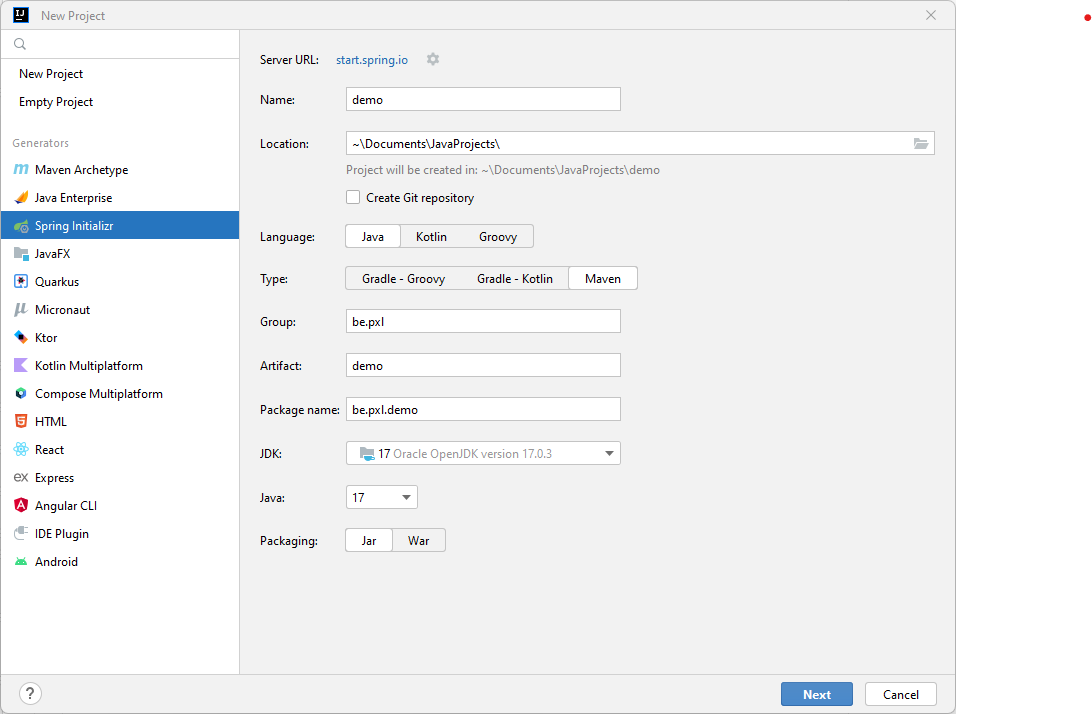
\includegraphics[width=\textwidth]{./images/chapter1/spring_initializer_intellij.png}

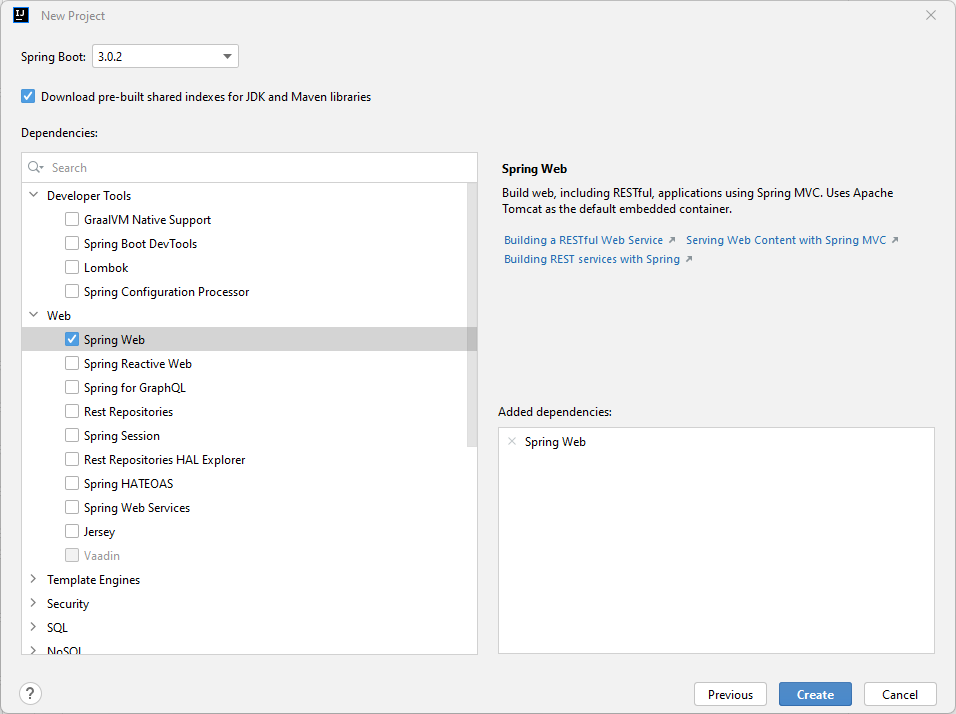
\includegraphics[width=\textwidth]{./images/chapter1/new_project.png}

We select Spring Web dependency. Spring Web uses Spring MVC. It is used for building RESTful Web Services. Spring MVC provides the annotation @RestController for classes that implement the REST endpoints.
To run a RESTful Web Service you need a web container. Spring Boot will automatically add an embedded Tomcat web container to your project. If you prefer another web container, you can update Spring Boot's configuration.
Finally Jackson is a popular third-party library for converting Java-objects to JSON and vice versa.

\begin{oefening}
Create the demo project. You can use the wizard in IntelliJ IDEA Ultimate or \url{https://start.spring.io/}.
\end{oefening}

\section{Running the demo project}

The starting point of a Spring Boot application is the class with the main-method and annotated with @SpringBootApplication.  This class can be found in the folder /src/main/java.  Spring Boot offers a lot of annotations to reduce the workload of developers.   

\begin{lstlisting}[frame=single]
package be.pxl.demo;

import org.springframework.boot.SpringApplication;
import org.springframework.boot.autoconfigure.SpringBootApplication;

@SpringBootApplication
public class DemoApplication {

    public static void main(String[] args) {
        SpringApplication.run(DemoApplication.class, args);
    }

}
\end{lstlisting}

By running the main-class you start your Spring Boot application. 

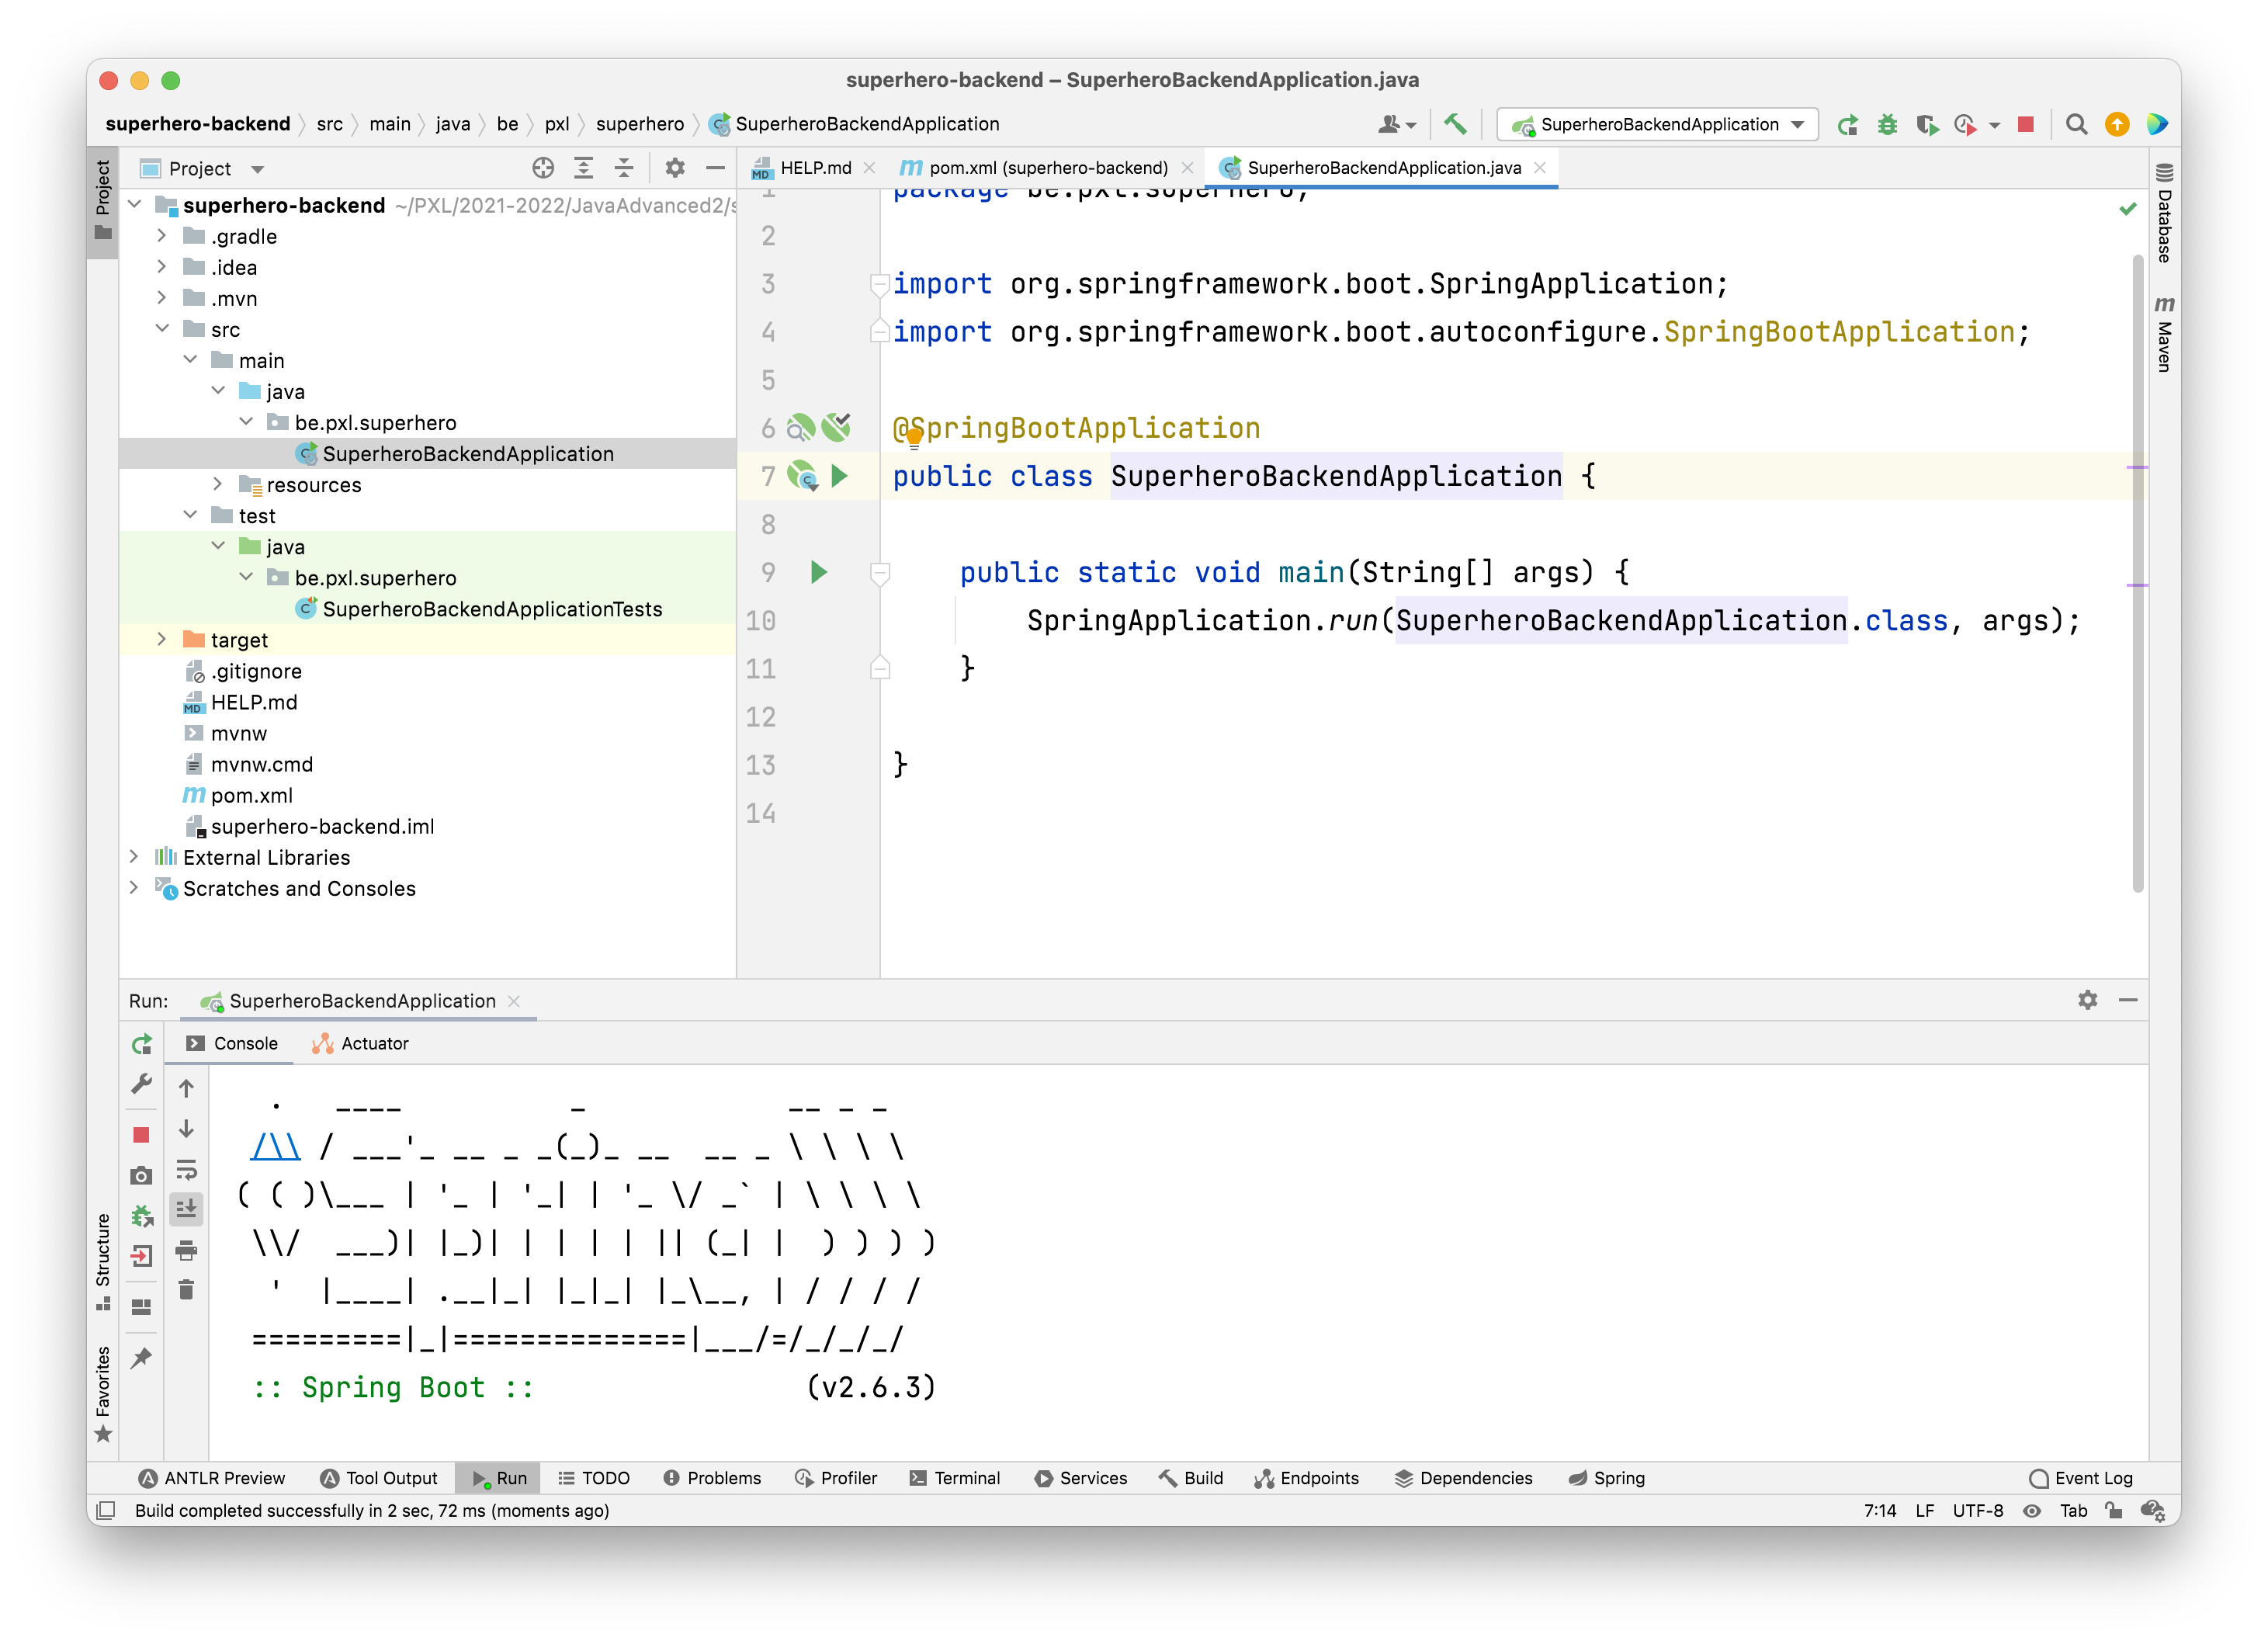
\includegraphics[width=\textwidth]{./images/chapter2/first-run.png}

Currently our Spring Boot application only shows a whitelabel error page. This error page is available when you perform a GET for URL \url{http://localhost:8080}.

\frame{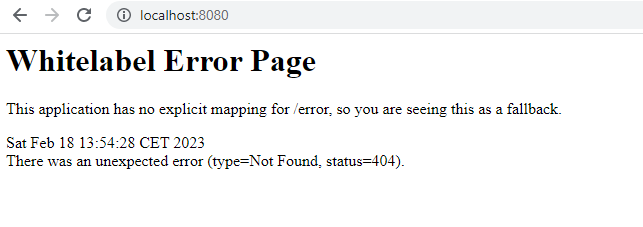
\includegraphics[width=\textwidth]{./images/chapter2/whitelabel_error_page.png}} 

Port 8080 is the default port. If this port is not available you will see an error message in Spring Boot's logging.

\begin{lstlisting}[frame=single]
***************************
APPLICATION FAILED TO START
***************************

Description:

Web server failed to start. Port 8080 was already in use.
\end{lstlisting}

The port number can be changed in the file application.properties. You have to add the property server.port here with the desired port number.

\begin{lstlisting}[frame=single]
server.port=8081
\end{lstlisting}

\subsection{The Maven pom file}

POM stands for \'Project Object Model\'. It is an XML representation of a Maven project held in a file named pom.xml. This file can be found in your project directory. The POM contains all necessary information about a project, as well as configurations of plugins to be used during the build process. We will cover Maven in chapter 3.

\begin{lstlisting}[frame=single]
<?xml version="1.0" encoding="UTF-8"?>
<project xmlns="http://maven.apache.org/POM/4.0.0" xmlns:xsi="http://www.w3.org/2001/XMLSchema-instance"
         xsi:schemaLocation="http://maven.apache.org/POM/4.0.0 https://maven.apache.org/xsd/maven-4.0.0.xsd">
    <modelVersion>4.0.0</modelVersion>
    <parent>
        <groupId>org.springframework.boot</groupId>
        <artifactId>spring-boot-starter-parent</artifactId>
        <version>3.0.2</version>
        <relativePath/> <!-- lookup parent from repository -->
    </parent>
    <groupId>be.pxl</groupId>
    <artifactId>demo</artifactId>
    <version>0.0.1-SNAPSHOT</version>
    <name>demo</name>
    <description>demo</description>
    <properties>
        <java.version>17</java.version>
    </properties>
    <dependencies>
        <dependency>
            <groupId>org.springframework.boot</groupId>
            <artifactId>spring-boot-starter-web</artifactId>
        </dependency>

        <dependency>
            <groupId>org.springframework.boot</groupId>
            <artifactId>spring-boot-starter-test</artifactId>
            <scope>test</scope>
        </dependency>
    </dependencies>

    <build>
        <plugins>
            <plugin>
                <groupId>org.springframework.boot</groupId>
                <artifactId>spring-boot-maven-plugin</artifactId>
            </plugin>
        </plugins>
    </build>
</project>
\end{lstlisting}

spring-boot-starter-parent is a starter project that provides the default configuration for spring-based applications. Here you choose the version of Spring Boot.

For large projects, managing the dependencies is not always easy. Spring Boot solves this problem by grouping certain dependencies together. These groups of dependencies are called starters. All Spring Boot starters are named following the same naming pattern. The all start with spring-boot-starter-*, where * indicates the purpose and functionality provided by the starter.

spring-boot-starter-web adds all the libraries we need to develop web components. An embedded server will be provided in the Spring Boot project. Therefore the environment where the Spring Boot project is executed does not need to have a pre-installed server. The default embedded server for Spring Boot is Tomcat. The Spring MVC framework which provides all classes for developing RESTful web services is also part of spring-boot-starter-web.

spring-boot-starter-test (with scope test) is the starter for testing Spring Boot applications with libraries including JUnit Jupiter, Hamcrest and Mockito.

\subsection{A Rest Controller}

RestControllers are used for making RESTful web services with the help of the @RestController annotation. The RestController allows to handle all HTTP methods such as GET, POST, DELETE, PUT. 

\begin{lstlisting}[frame=single]
package be.pxl.demo.api;

import jakarta.annotation.PostConstruct;
import org.springframework.web.bind.annotation.GetMapping;
import org.springframework.web.bind.annotation.RestController;

import java.util.ArrayList;
import java.util.List;
import java.util.Random;

@RestController
public class GreetingController {

    private final List<String> messages = new ArrayList<>();
    private static final Random RANDOM = new Random();

    @PostConstruct
    public void init() {
        messages.add("Peek-a-boo!");
        messages.add("Howdy-doody!");
        messages.add("My name's Ralph, and I'm a bad guy.");
        messages.add("I come in peace!");
        messages.add("Put that cookie down!");

    }

    @GetMapping("/hello")
    public String doGreeting() {
        return messages.get(RANDOM.nextInt(messages.size()));
    }
}
\end{lstlisting}

When Spring's DispatcherServlet receives a request for the URL /hello it looks for the correct @RestController to handle the request. The annotation @RequestMapping is used for mapping all incoming HTTP request URLs to the corresponding controller methods. The DispatcherServlet will be discussed in detail in a later chapter. The Spring container is responsible for managing an instance of the @RestController. When an instance of our GreetingController is created,  the init method is called to initialise all possible greetings.  The @GetMapping is a specialized version of @RequestMapping and is used for methods handling HTTP  GET requests.  Therefore, when we call the URL \url{http://localhost:8080/hello}, the method doGreeting() in the GreetingController will handle the request and return a greeting message in text format.

\begin{oefening}
Create the package \textit{be.pxl.demo.api}. Add the class \textbf{GreetingController} in this package. Restart the Spring Boot application and open the URL \url{http://localhost:8080/hello} in a browser.
\end{oefening}

\subsection{Auto-configuration}

Spring Boot auto-configuration attempts to automatically configure your Spring application based on the dependencies that you have added.
To gain some insight in this auto-configuration let's add a line in the application.properties file. This file can be found in the directory /src/main/resources. 

\begin{lstlisting}
logging.level.org.springframework=debug
\end{lstlisting}

logging.level.org.springframework is a application properties. A list of all available application properties can be found at \url{https://docs.spring.io/spring-boot/docs/current/reference/html/application-properties.html}.

\begin{oefening}
Add the line above to the application.properties file and restart the Spring Boot application.
\end{oefening}

In the console you will find all the auto-configuration Spring Boot is doing.

\subsection{@SpringBootApplication}

Java annotations are a mechanism for adding metadata information to our source code. An annotation processor processes these annotations at compile time or runtime to provide functionality such as code generation, error checking, etc.

@SpringBootApplication annotation is used to enable following three features:
\begin{itemize}
\item @EnableAutoConfiguration: enable Spring Boot’s auto-configuration mechanism
\item @ComponentScan: enable @Component scan on the package where the application is located
\item @Configuration: allow to register extra beans in the context or import additional configuration classes
\end{itemize}


\section{Components and dependency injection}

All our REST backend applications will consist of 3 layers:
 router-layer (or API-layer), service- or business-layer and persistence-layer.

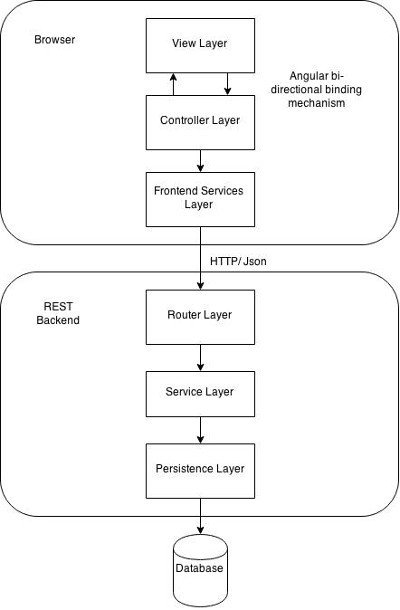
\includegraphics[scale=0.6]{./images/chapter1/spring-architecture.jpeg} 

\begin{itemize}
\item \textbf{Router- or presentation layer:}  Handling and processing HTTP requests,  translating JSON parameters to objects,  authentication of users and protecting data from maleficent users,  ... .
\item \textbf{Service- or business logic layer:} This layer contains the business logic, the core functionality of your application. All calculations, decisions, evaluations, data processing,... are handled by this layer. 
\item \textbf{Data- or persistence layer:} This layer is responsible for interacting with the database.  This layer stores and retrieves the application data in the database.
\end{itemize}

The typical components for each layer are annotated.  These annotated components are managed by Spring. Developers are not responsible for creating the objects of these component classes. The actual objects are created and injected by Spring wherever we need them. In later chapters we will discuss the concept of dependency injection in detail.

The annotations for the Spring components we will use are:
\begin{itemize}
\item @Component: generic annotation for all components managed by Spring
\item @RestController: indicate the components in the API layer
\item @Service: indicate the components in the service layer
\item @Repository: indicate the components in the persistence layer
\end{itemize}

All of these application components (@Component, @Service, @Repository, @Controller, and others) are automatically registered as Spring Beans.

Here is the definition of beans from the Spring framework documentation:

\fcolorbox{black}[HTML]{E9F0E9}{\parbox{\textwidth}{%
\noindent In Spring, the objects that form the backbone of your application and that are managed by the Spring IoC container are called beans. A bean is an object that is instantiated, assembled, and otherwise managed by a Spring IoC container.}}

IoC or Inversion of Control is the process in which an object defines its dependencies without creating them. The IoC container is responsible for constructing the dependencies.

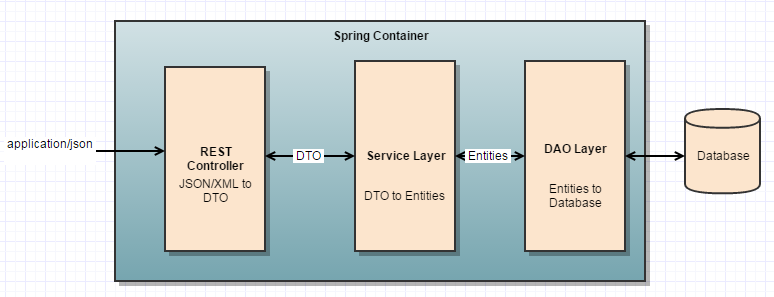
\includegraphics[width=\textwidth]{./images/Spring-REST-Web-Services.png} 

The image shows all the layers that we develop in our REST backend applications. The RestController in the API layer provides REST endpoints. The API layer communicates via DTOs or Data Transfer Objects with the service layer. The service layer implements all business logic. DTOs are mapped to entity-objects and passed along the persistence layer. The persistence layer is responsible for storing the entity-objects in the database.

The Spring container is at the core of the Spring Framework. The container is responsible for creating and managing the objects for classes annotated with @Service, @Repository,... The container will provide these objects (beans) when they are needed by other beans.


\section{DevOps Tools for Java Developers}

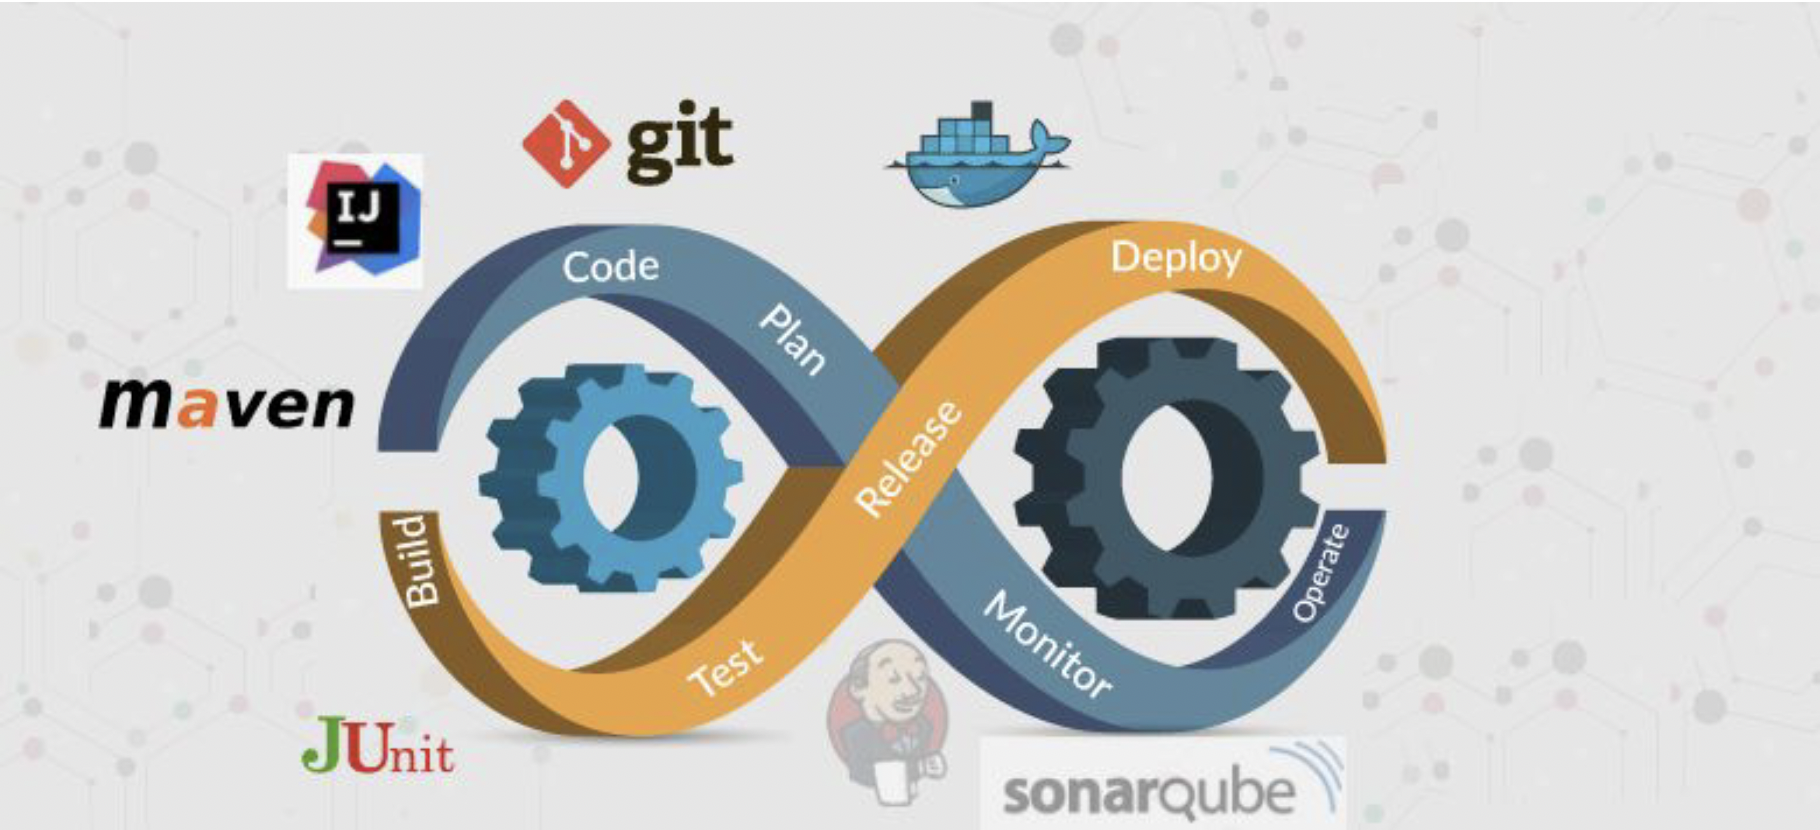
\includegraphics[width=\textwidth]{./images/chapter1/devops.png}  
 

\chapter{Creating a Spring Boot application}

\fcolorbox{black}[HTML]{E9F0E9}{\parbox{\textwidth}{%
\noindent \textbf{Learning goals}\\
The junior-colleague
\begin{enumerate}[nolistsep]
\item can identify the different components in a Spring Boot application
\item can explain what REST is
\item can explain what an entity-class is
\item can create a RestController
\item can run a Spring Boot application
\item can enable CORS support in a Spring Boot application
\item ...
\end{enumerate}}}


\section{Creating a Spring Boot project}

This chapter will guide you through the implementation of your first Spring Boot application. You will create a RESTful webservice for managing the information of a ``Super Hero Company''. We will implement REST endpoints for creating, updating and deleting superheroes. Later you will add functionality to create, update and delete missions for the superheroes.

We use Spring Intializr to bootstrap this Spring Boot application. 

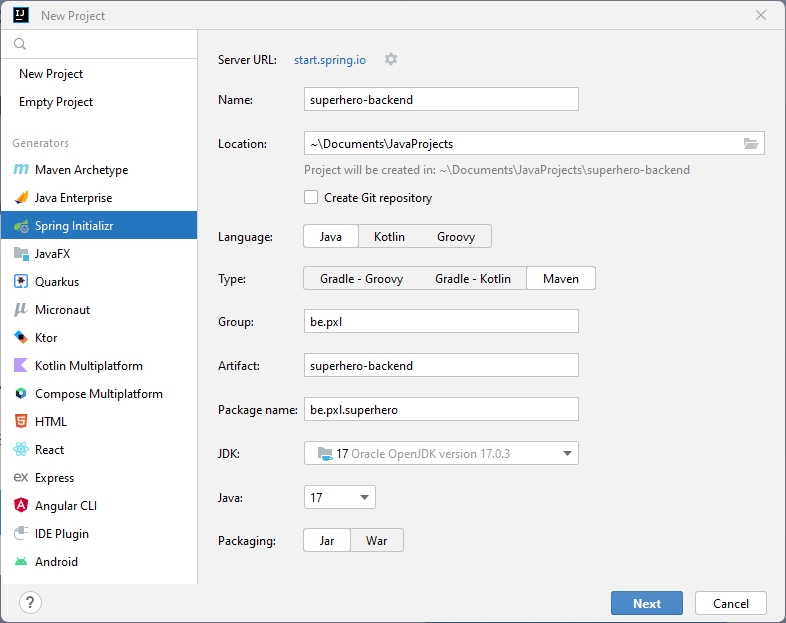
\includegraphics[width=\textwidth]{./images/chapter2/new_project.png} 

In the first screen of the wizard you have to provide metadata about your project.  The information you have to provide is:
\begin{itemize}
\item \textbf{Group:} unique identification of your project across all projects.  A group follows Java's package name rules. It also infers the root package name to use.
\item \textbf{Artifact:} the name of a project artifact without version.  It also infers the name of the project.
\item \textbf{Name:} display name of the project that also determines the name of your Spring Boot application. For instance,  if the name of your project is my-app, the generated project will have a MyAppApplication class
\item \textbf{Description:} description of the project.
\item \textbf{Package Name:} root package of the project. If not specified, the value of the group attribute is used
\item \textbf{Packaging:} project packaging.  You can choose either jar or war projects.
\item \textbf{Java Version:} the Java version to use
\item \textbf{Language:} the programming language to use
\end{itemize}

During this course we use Maven as build tool for our projects. In the next chapter we will discuss Maven into detail.

Our backend provides a REST API. A clear explanation about REST can be found at \href{https://www.codecademy.com/article/what-is-rest.}{codecademy}.  To implement REST endpoints we need some third-party libraries: Spring MVC, Tomcat and Jackson. All these libraries are bundled in one starter: \textbf{spring-boot-starter-web}.

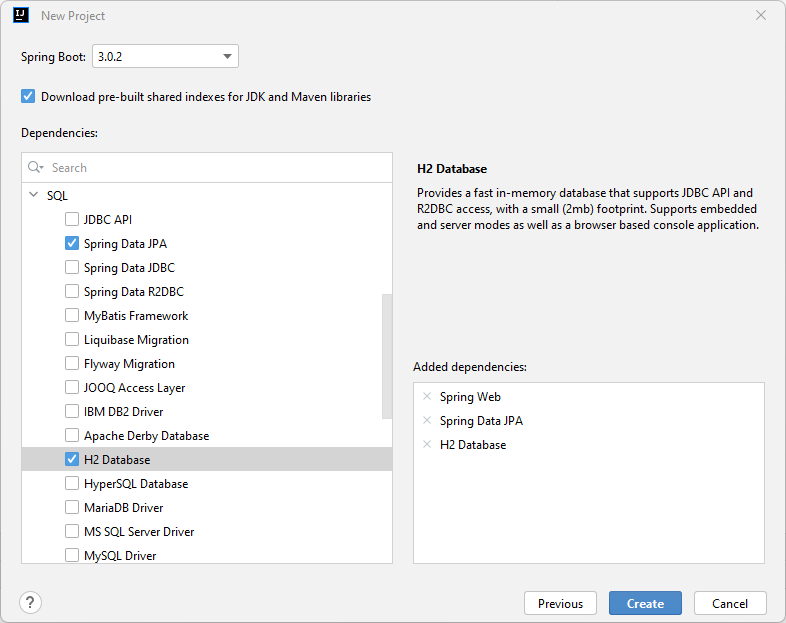
\includegraphics[width=\textwidth]{./images/chapter2/new_project_metadata.png}

Besides Spring Web, we add Spring Data JPA to the project. Using this starter depencency we can use JPA (the Java or Jakarta Persistence API) to access a database. 
The dependency spring-boot-starter-data-jpa will be added to the pom.xml file. This one starter adds different libraries for easily accessing a database.
Finaly the H2 Database dependency is added. This is an in-memory database 
and you need zero configuration to use this database. This is nice for fast prototyping, but all your data is lost once you restart the application. All database related technologies will be explained in detail during this course. 

\begin{oefening}
Create your superhero Spring Boot project. You can use the wizard in IntelliJ IDEA Ultimate or \url{https://start.spring.io/}.
\end{oefening}

\section{Storing and retrieving data}

\subsection{Entity-class Superhero}

First we need a class for respresenting the objects that are stored and retrieved from the database. Each object of this class will represent one row of a table in the relational database.
We implement the class Superhero. To save Superhero-objects to the database and retrieve Superhero-objects from the database, we annotate this class and make it an entity-class. 


\includegraphics[scale=0.5]{./images/chapter2/superman.jpeg} 

Here is the entity-class Superhero:

\begin{lstlisting}[frame=single]
package be.pxl.superhero.domain;

import jakarta.persistence.Entity;
import jakarta.persistence.GeneratedValue;
import jakarta.persistence.GenerationType;
import jakarta.persistence.Id;
import jakarta.persistence.Table;

@Entity
@Table(name="superheroes")
public class Superhero {
	
	@Id
	@GeneratedValue(strategy = GenerationType.IDENTITY)
	private Long id;
	
	private String firstName;
	private String lastName;
	private String superheroName;

	public Superhero() {
		// JPA only
	}

	public Superhero(String firstName, String lastName, String superheroName) {
		this.firstName = firstName;
		this.lastName = lastName;
		this.superheroName = superheroName;
	}

	public Long getId() {
		return id;
	}

	public String getFirstName() {
		return firstName;
	}

	public void setFirstName(String firstName) {
		this.firstName = firstName;
	}

	public String getLastName() {
		return lastName;
	}

	public void setLastName(String lastName) {
		this.lastName = lastName;
	}

	public String getSuperheroName() {
		return superheroName;
	}

	public void setSuperheroName(String superheroName) {
		this.superheroName = superheroName;
	}

	@Override
	public String toString() {
		return superheroName;
	}
}
\end{lstlisting}

The annotation @Entity indicates that the class is actually an entity-class.  Spring is able to automatically generate the database table (superheroes) with all its fields in the H2 database. 
The primary key of the table is marked with the annotation @Id.  Further, with the annotation @GeneratedValue(strategy = GenerationType.IDENTITY) we don't have to assign the primary keys to the objects. The database itself is responsible for generating and assigning the primary keys.

\begin{oefening}
Add the entity class Superhero to your project.  Create the package package \textit{be.pxl.superhero.domain} for this class.
\end{oefening}

\subsection{Repository}

To execute queries in the database we need an extra class (or interface) called a \textbf{repository}. Spring is able to automatically generate database queries. When you extend the interface JpaRepository, simple queries are already available without writing one line of code. 
The generic interface JpaRepository only needs to know which data it must store and retrieve.
Therefore it needs to know the name of the entity-class and the data type of the primary key of the entity-class. 

\begin{lstlisting}[frame=single]
package be.pxl.superhero.repository;

import be.pxl.superhero.domain.Superhero;
import org.springframework.data.jpa.repository.JpaRepository;
import org.springframework.stereotype.Repository;

@Repository
public interface SuperheroRepository extends JpaRepository<Superhero, Long> {
}
\end{lstlisting}

When you open the documentation of the generic interface JpaRepository, you can see which functionality is available for the developer.

\begin{oefening}
Add the repository-interface SuperheroRepository to the project.  Create the package  \textit{be.pxl.superhero.repository} for this interface.
\end{oefening}

\subsection{Service-layer}

The classes in the service-layer are responsible for the business logic. These classes use the repositories to save and retrieve data from the database.  It is good practice to provide an interface for every class in the service-layer (service-class). 
The service-classes may never return entity-objects. We need DTOs (Data Transfer Objects) to pass data from the service-layer to the API-layer.

\begin{lstlisting}[frame=single]
package be.pxl.superhero.service;

import be.pxl.superhero.api.SuperheroDTO;
import be.pxl.superhero.api.SuperheroRequest;

import java.util.List;

public interface SuperheroService {

	List<SuperheroDTO> findAllSuperheroes();

	SuperheroDTO findSuperheroById(Long superheroId);

	Long createSuperhero(SuperheroRequest superheroRequest);

	SuperheroDTO updateSuperhero(Long superheroId, SuperheroRequest superheroRequest);

	boolean deleteSuperhero(Long superheroId);
}
\end{lstlisting}


\begin{lstlisting}[frame=single]
package be.pxl.superhero.api;

import be.pxl.superhero.domain.Superhero;

public class SuperheroDTO {

	private final Long id;
	private final String firstName;
    private final String lastName;
    private final String superheroName;

    public SuperheroDTO(Superhero superhero) {
	   this.id = superhero.getId();
        this.firstName = superhero.getFirstName();
        this.lastName = superhero.getLastName();
        this.superheroName = superhero.getSuperheroName();
    }

	public Long getId() {
		return id;
	}

	public String getFirstName() {
        return firstName;
    }

    public String getLastName() {
        return lastName;
    }

    public String getSuperheroName() {
        return superheroName;
    }

}
\end{lstlisting}

\begin{lstlisting}[frame=single]
package be.pxl.superhero.api;

public class SuperheroRequest {

	private String firstName;
	private String lastName;
	private String superheroName;

	public SuperheroRequest(String firstName, String lastName, String superheroName) {
		this.firstName = firstName;
		this.lastName = lastName;
		this.superheroName = superheroName;
	}

	public String getFirstName() {
		return firstName;
	}

	public void setFirstName(String firstName) {
		this.firstName = firstName;
	}

	public String getLastName() {
		return lastName;
	}

	public void setLastName(String lastName) {
		this.lastName = lastName;
	}

	public String getSuperheroName() {
		return superheroName;
	}

	public void setSuperheroName(String superheroName) {
		this.superheroName = superheroName;
	}

}

\end{lstlisting}

The class SuperheroServiceImpl, annotated with @Service, provides the implementation for the interface SuperheroService.
All CRUD-operations (create-read-update-delete) for Superhero-objects are provided here.
In the class SuperheroServiceImpl all business logic can be implemented.  If we, for example, have to check that the superheroname of a superhero is unique, this class is the place to implement these checks.  (At the moment we will not yet implement this business rule!)

The SuperheroRepository is autowired in the SuperheroServiceImpl. Hence the service-class can save and retrieve data from the database with the help from this repository. 


\begin{lstlisting}[frame=single]
package be.pxl.superhero.service.impl;

import be.pxl.superhero.api.SuperheroDTO;
import be.pxl.superhero.api.SuperheroRequest;
import be.pxl.superhero.domain.Superhero;
import be.pxl.superhero.exception.ResourceNotFoundException;
import be.pxl.superhero.repository.SuperheroRepository;
import be.pxl.superhero.service.SuperheroService;
import org.springframework.stereotype.Service;

import java.util.List;
import java.util.stream.Collectors;

@Service
public class SuperheroServiceImpl implements SuperheroService {

	private final SuperheroRepository superheroRepository;

	public SuperheroServiceImpl(SuperheroRepository superheroRepository) {
		this.superheroRepository = superheroRepository;
	}

	public List<SuperheroDTO> findAllSuperheroes() {
		return superheroRepository.findAll()
				.stream().map(SuperheroDTO::new)
				.toList();
	}

	public SuperheroDTO findSuperheroById(Long superheroId) {
		return superheroRepository.findById(superheroId)
		         .map(SuperheroDTO::new)
				.orElseThrow(() -> new ResourceNotFoundException("Superhero", "ID", superheroId));
	}

	public Long createSuperhero(SuperheroRequest superheroRequest) {
		Superhero superhero = new Superhero();
		superhero.setFirstName(superheroRequest.getFirstName());
		superhero.setLastName(superheroRequest.getLastName());
		superhero.setSuperheroName(superheroRequest.getSuperheroName());
		Superhero newSuperhero = superheroRepository.save(superhero);
		return newSuperhero.getId();
	}

	public SuperheroDTO updateSuperhero(Long superheroId, SuperheroRequest superheroRequest) {
		return superheroRepository.findById(superheroId).map(superhero -> {
			superhero.setFirstName(superheroRequest.getFirstName());
			superhero.setLastName(superheroRequest.getLastName());
			superhero.setSuperheroName(superheroRequest.getSuperheroName());
			return new SuperheroDTO(superheroRepository.save(superhero));
		}).orElseThrow(() -> new ResourceNotFoundException("Superhero", "id", superheroId));
	}

	public boolean deleteSuperhero(Long superheroId) {
		return superheroRepository.findById(superheroId)
				.map(superhero -> {
					superheroRepository.delete(superhero);
					return true;
				}).orElseThrow(() -> new ResourceNotFoundException("Superhero", "id", superheroId));

	}
}
\end{lstlisting}

\begin{lstlisting}
package be.pxl.superhero.exception;

public class ResourceNotFoundException extends RuntimeException {
    public ResourceNotFoundException(String resource, String field, String value) {
        super("Not found: " + resource + " with " + field + "=" + value);
    }

    public ResourceNotFoundException(String resource, String field, long value) {
        this(resource, field, Long.toString(value));
    }
}
\end{lstlisting}

\begin{oefening}
Create the package \textit{be.pxl.superhero.api} and add the request-object SuperheroRequest and the DTO SuperheroDTO.  These classes are used for communication with the API-layer. 
Add the interface SuperheroService en the implementation SuperheroServiceImpl to your project. The interface is located in the package \textit{be.pxl.superhero.service}. The implementation is located in the package \textit{be.pxl.superhero.service.impl}. Finally you add the exception-class  ResourceNotFoundException to the package \textit{be.pxl.superhero.exception}.
\end{oefening}

\subsection{REST controller}

Now we can add the REST endpoints for creating, updating, deleting and retrieving superheroes. 

For creating a new superhero we offer a POST-request with a requestbody in JSON-format. This requestbody holds all information about the new superhero.  You already added the class SuperheroRequest to the project. This class is used for mapping the data of the requestbody to an object.

To test the implemented REST endpoints,  you can use postman (https://www.postman.com/) or insomnia (https://insomnia.rest/). 

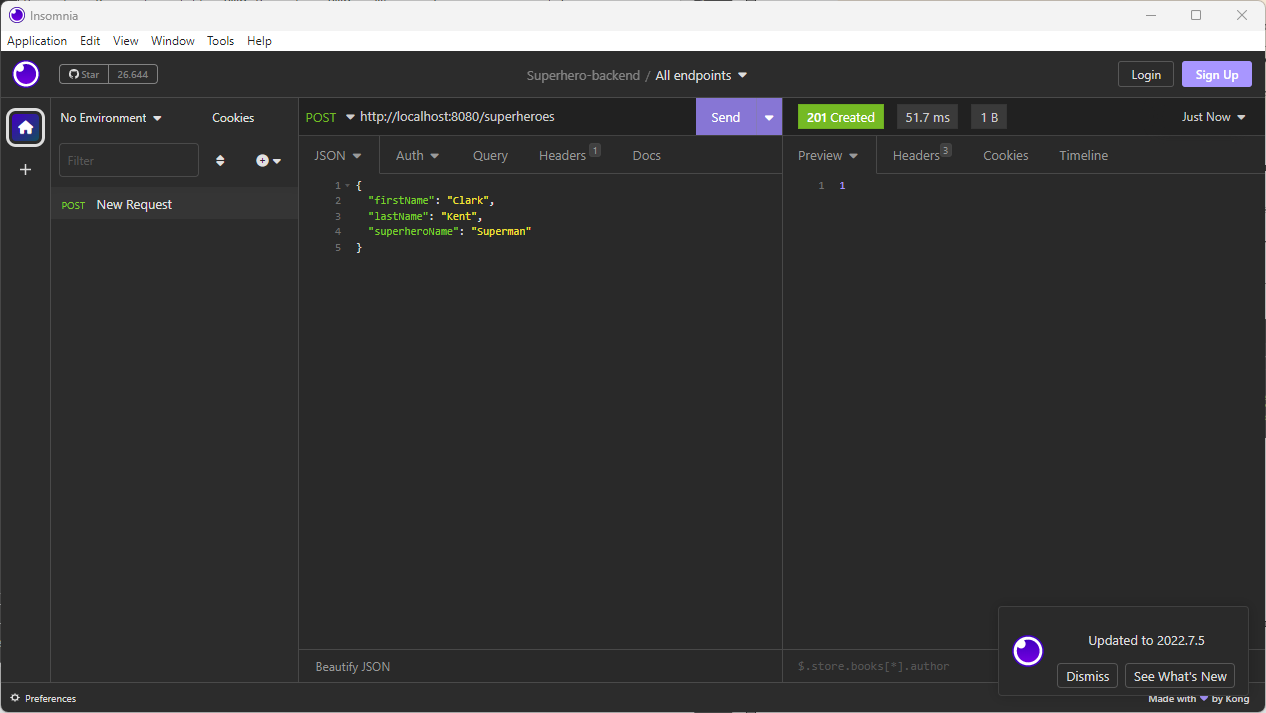
\includegraphics[width=\textwidth]{./images/chapter2/post-request-insomnia.png} 

Look at the method createSuperhero in the class below. The datatype of the parameter is SuperheroRequest and is annotated with @RequestBody.  Therefore the body of the HTTP request in JSON-format is mapped to an object of the class (when the fields correspond). 

The RestController uses the implementation of SuperheroService to map this SuperheroRequest to a Superhero-entity. Finally, the SuperheroRepository is responsible for saving the Superhero-entity in the database. 


\begin{lstlisting}[frame=single]
package be.pxl.superhero.api;

import be.pxl.superhero.service.SuperheroService;
import org.springframework.http.HttpStatus;
import org.springframework.http.ResponseEntity;
import org.springframework.web.bind.annotation.DeleteMapping;
import org.springframework.web.bind.annotation.GetMapping;
import org.springframework.web.bind.annotation.PathVariable;
import org.springframework.web.bind.annotation.PostMapping;
import org.springframework.web.bind.annotation.PutMapping;
import org.springframework.web.bind.annotation.RequestBody;
import org.springframework.web.bind.annotation.RequestMapping;
import org.springframework.web.bind.annotation.RestController;

import java.util.List;

@RestController
@RequestMapping("/superheroes")
public class SuperheroController {

	private final SuperheroService superheroService;

	public SuperheroController(SuperheroService superheroService) {
		this.superheroService = superheroService;
	}

	@GetMapping
	public List<SuperheroDTO> getSuperheroes() {
		return superheroService.findAllSuperheroes();
	}

	@GetMapping("/{superheroId}")
	public SuperheroDTO getSuperheroById(@PathVariable Long superheroId) {
		return superheroService.findSuperheroById(superheroId);
	}
	
	@PostMapping
	public ResponseEntity<Long> createSuperhero(@RequestBody SuperheroRequest superheroRequest) {
		return new ResponseEntity<>(superheroService.createSuperhero(superheroRequest), HttpStatus.CREATED);
	}
	
	@PutMapping("/{superheroId}")
	public SuperheroDTO updateSuperhero(@PathVariable Long superheroId, @RequestBody SuperheroRequest superheroRequest) {
		return superheroService.updateSuperhero(superheroId, superheroRequest);
	}
	
	@DeleteMapping("/{superheroId}")
	public ResponseEntity<Void> deleteSuperhero(@PathVariable Long superheroId) {
		boolean deleted = superheroService.deleteSuperhero(superheroId);
		return deleted? new ResponseEntity<>(HttpStatus.OK) : new ResponseEntity<>(HttpStatus.BAD_REQUEST);
	}
}
\end{lstlisting}

\begin{oefening}
Add @RestController SuperheroController to your Spring Boot application.  Restart the project and create a new superhero with insomnia or postman.  Next you call the REST endpoint to retrieve all superheroes or retrieve the superhero by id. 

Here is the json-format to create a superhero:
\begin{lstlisting}
{
	"firstName": "Clark",
	"lastName": "Kent",
	"superheroName": "Superman"
}
\end{lstlisting}
\end{oefening}

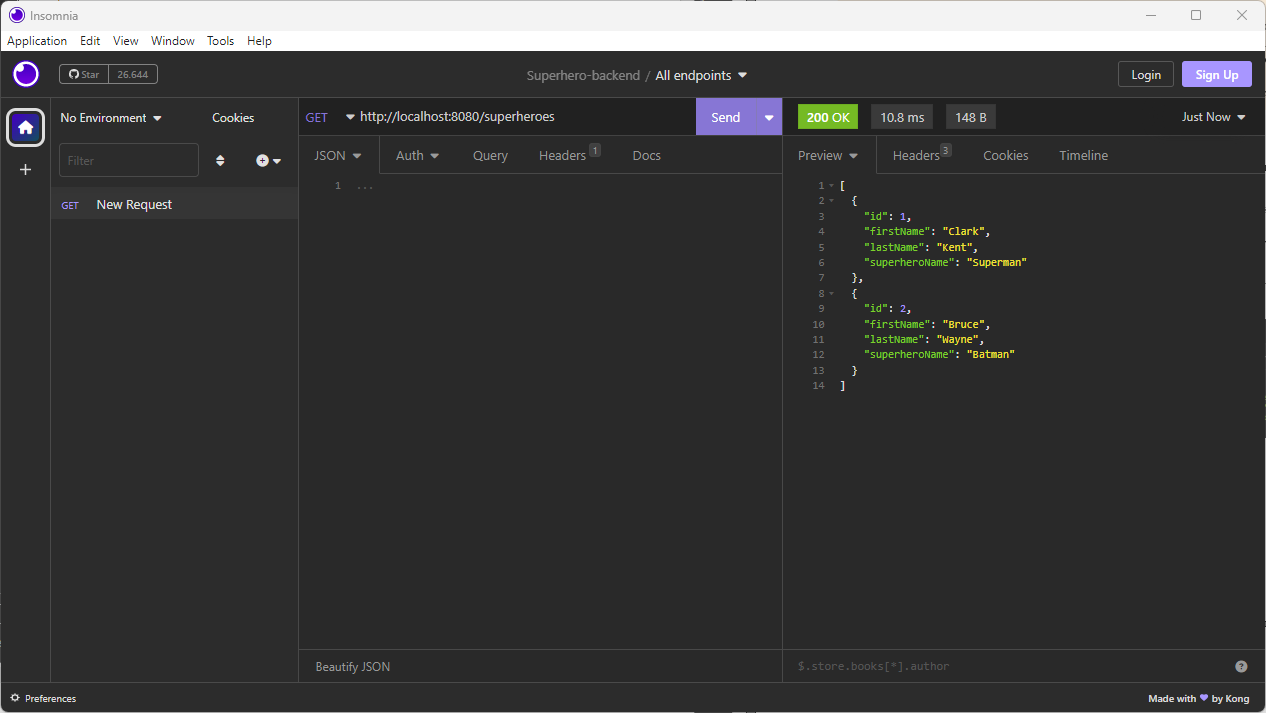
\includegraphics[width=\textwidth]{./images/chapter2/get-request-insomnia.png}

\section{URL context path}

When you want to add a prefix e.g. /api to all the URLs provided by the application, you can add the following key-value-pair in the file application.properties:

\begin{lstlisting}[frame=single]
server.servlet.context-path=/api
\end{lstlisting}


\begin{oefening}
Change the context-path of your Spring Boot application. The prefix /api should be used for the application.  Restart the application and test the endpoints.
\end{oefening}

\section{Resource not found}

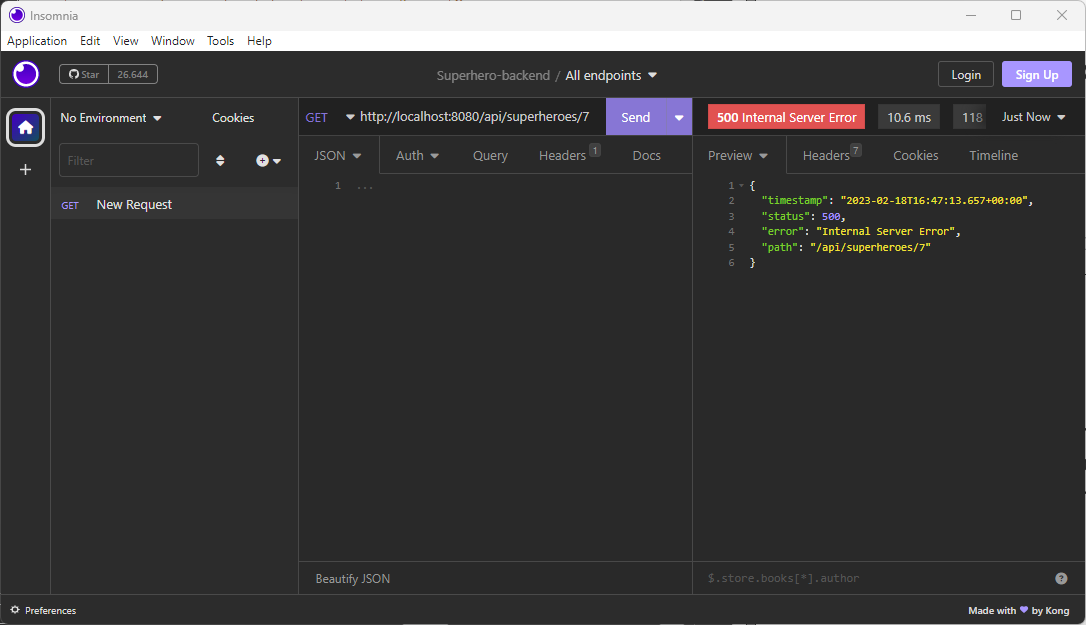
\includegraphics[width=\textwidth]{./images/chapter2/not_found_1.png}

\begin{lstlisting}
package be.pxl.superhero.exception;

import org.springframework.http.HttpStatus;
import org.springframework.web.bind.annotation.ResponseStatus;

@ResponseStatus(HttpStatus.NOT_FOUND)
public class ResourceNotFoundException extends RuntimeException {
    public ResourceNotFoundException(String resource, String field, String value) {
        super("Not found: " + resource + " with " + field + "=" + value);
    }

    public ResourceNotFoundException(String resource, String field, long value) {
        this(resource, field, Long.toString(value));
    }
}
\end{lstlisting}

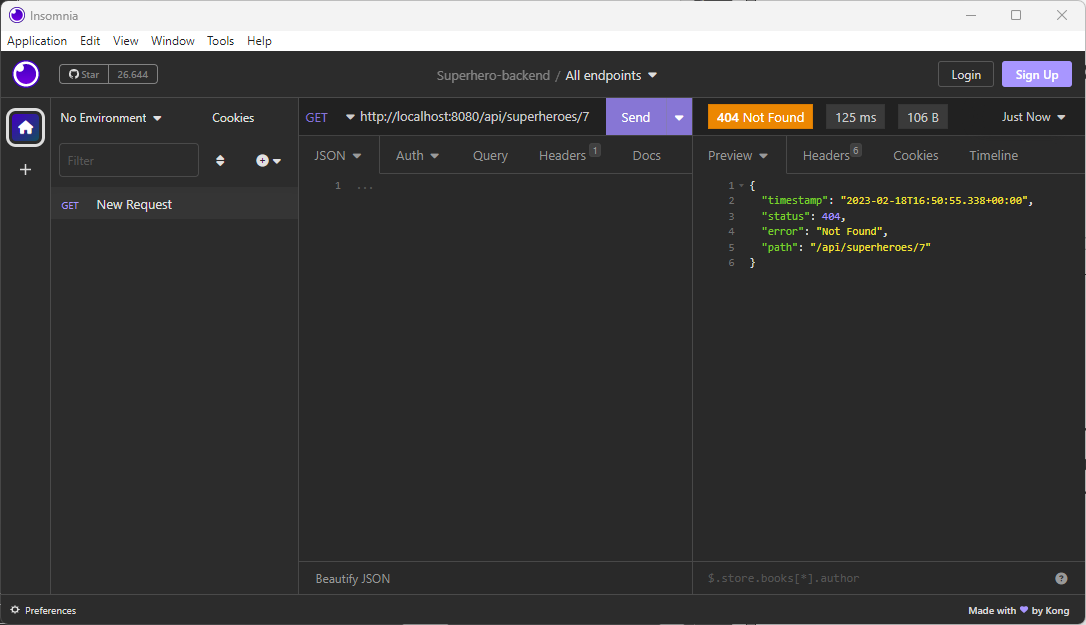
\includegraphics[width=\textwidth]{./images/chapter2/not_found_2.png}

\section{API documentation}

Documentation about your Superhero REST API can be made available with the third-party library. You must add following dependencies to the file pom.xml.

\begin{lstlisting}[language=xml]
<dependency>
	<groupId>org.springdoc</groupId>
	<artifactId>springdoc-openapi-starter-webmvc-ui</artifactId>
	<version>2.0.0</version>
</dependency>
<dependency>
	<groupId>org.springframework.boot</groupId>
	<artifactId>spring-boot-starter-validation</artifactId>
</dependency>
\end{lstlisting}

This documentation in xml-format that can be found by the URL \url{http://localhost:8080/api/v3/api-docs} is not user-friendly.  However, if you open the URL \url{http://localhost:8080/api/swagger-ui.html} in you browser, you can see a user-friendly swagger page where you can even test your API.


\begin{tcolorbox}[colback=blue!5!white,colframe=blue!75!black,title=H2 database]
Our H2 in-memory database disappears when you close the application and all data is lost.
You can use files to permanently save the data.  If you want to inspect the data of your in-memory database, you can add the following property to the file application.properties (located in the resources folder)
\begin{lstlisting}[frame=single]
spring.h2.console.enabled=true
\end{lstlisting}
When you start the Spring Boot application, you are given a unique identifier for your database.  
\begin{lstlisting}[frame=single]
H2 console available at '/h2-console'. Database available at 'jdbc:h2:mem:f5f92e54-3aff-4986-9d00-a0028b0eb6ed'
\end{lstlisting}
When you open the URL \url{http://localhost:8080/api/h2-console} in a browser and fill in the unique id and the username ``sa'' (the password field is left blank),  you are given access to the tables and data of your database. 

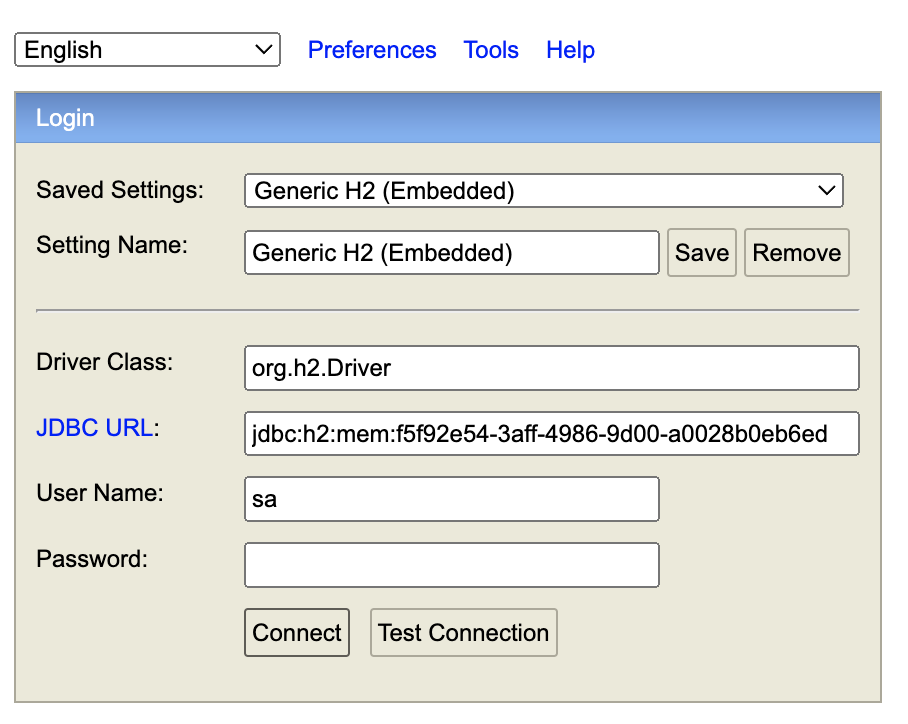
\includegraphics[width=\textwidth]{./images/chapter2/h2-database.png} 

More information about the H2 database is available at \url{https://www.baeldung.com/spring-boot-h2-database}.
\end{tcolorbox}

\section{Frontend}

A frontend for the superhero application written in Angular can be found at github.  (Credits to: \url{https://github.com/shoul10}).


 \fcolorbox{black}[HTML]{ADD8E6}{\parbox{\textwidth}{%
\noindent \textbf{Source code}\\
The frontend code is available at: \url{https://github.com/custersnele/superhero-frontend.git}
}}

Our backend should support CORS to make the API available for the angular frontend.  Cross-origin resource sharing (CORS) is a W3C specification used by most browsers.  

Add the following configuration to your project to support CORS.

\begin{lstlisting}[frame=single]
package be.pxl.superhero.config;

import org.springframework.context.annotation.Configuration;
import org.springframework.web.servlet.config.annotation.CorsRegistry;
import org.springframework.web.servlet.config.annotation.WebMvcConfigurer;

@Configuration
public class WebMvcConfig implements WebMvcConfigurer {
    private static final long MAX_AGE_SECS = 3600;

    @Override
    public void addCorsMappings(CorsRegistry registry) {
        registry.addMapping("/**")
                .allowedOrigins("*")
                .allowedMethods("HEAD", "OPTIONS", "GET", "POST", "PUT", "PATCH", "DELETE")
                .maxAge(MAX_AGE_SECS);        
    }
}
\end{lstlisting}

\begin{oefening}
Add CORS support to your project. The class WebMvcConfig will be located in the package  \textit{be.pxl.superhero.config}.  Restart the Spring Boot application.
Download the frontend code from github and open it in a  development environment (e.g.  WebStorm).  Start the frontend application (ng serve) and create, update and delete your superheroes.
\end{oefening}

\section{Records}

The Java record class type makes DTOs even more easy. It allows us to reduce boilerplate code. 

For example, this record class:

\begin{lstlisting}
package be.pxl.superherobackend.api;

public record SuperheroDTO (Long id, String firstName, String lastName, String superheroName) {
}
\end{lstlisting} 

is equal to this traditional Java class:

\begin{lstlisting}
package be.pxl.superherobackend.api;

public class SuperheroDTO {
    private final Long id;
    private final String firstName;
    private final String lastName;
    private final String superheroName;

    public SuperheroDTOFull(Long id, String firstName, String lastName, String superheroName) {
        this.id = id;
        this.firstName = firstName;
        this.lastName = lastName;
        this.superheroName = superheroName;
    }

    public Long getId() {
        return id;
    }

    public String getFirstName() {
        return firstName;
    }

    public String getLastName() {
        return lastName;
    }

    public String getSuperheroName() {
        return superheroName;
    }

    @Override
    public boolean equals(Object o) {
        if (this == o) return true;
        if (o == null || getClass() != o.getClass()) return false;

        SuperheroDTO that = (SuperheroDTO) o;

        if (id != null ? !id.equals(that.id) : that.id != null) return false;
        if (firstName != null ? !firstName.equals(that.firstName) : that.firstName != null) return false;
        if (lastName != null ? !lastName.equals(that.lastName) : that.lastName != null) return false;
        return superheroName != null ? superheroName.equals(that.superheroName) : that.superheroName == null;
    }

    @Override
    public int hashCode() {
        int result = id != null ? id.hashCode() : 0;
        result = 31 * result + (firstName != null ? firstName.hashCode() : 0);
        result = 31 * result + (lastName != null ? lastName.hashCode() : 0);
        result = 31 * result + (superheroName != null ? superheroName.hashCode() : 0);
        return result;
    }

    @Override
    public String toString() {
        return "SuperheroDTO{" +
                "id=" + id +
                ", firstName='" + firstName + '\'' +
                ", lastName='" + lastName + '\'' +
                ", superheroName='" + superheroName + '\'' +
                '}';
    }
}

\end{lstlisting}

A record class is a concise way to define an object that is shallowly immutable. The values inside a record are called record components. These are declared in the header of the record. Shallowly immutable means that the references that the immutable instance hold cannot change, but the values inside the referred instance can change.

It is possible to override the constructor in a record class.

\begin{oefening}
Replace SuperheroDTO and SuperheroRequest with record classes. Fix the code and test your application.
\end{oefening}
  

\chapter{Logging}


\section{Logging Framework}

A logging framework is a utility specifically designed to standardize the process of logging in your application.  Logging is very important for debugging and identifying performance hot spots in an application, as well as getting a sense of how your application operates.  The following recommendations about logging can be find in OWASP Logging Guide \footnote{\url{https://owasp.org/www-pdf-archive/OWASP_Logging_Guide.pdf}}:

\begin{itemize}
\item Why log?
\begin{itemize}
\item identify security incidents
\item identify fraudulent activity
\item identify operational and longterm problems
\item ensure compliance with laws,rules and regulations
\end{itemize}
\item What is commonly logged ?
\begin{itemize}
\item Client requests and server responses
\item Account activities (login, logout, change password etc.)
\item Usage information (transaction types and sizes, generated traffic etc.)
\item Significant operational actions such as application startup and shutdown, application failures, and major application configuration changes. This can be used to identify security compromises and operational failures.
\end{itemize}
\end{itemize}

Much of this info can only be logged by the applications themselves. This is especially true for applications used through encrypted network communications. Therefore we need a standardized process of logging where log-files can be archived easily.

\section{Log levels}

\begin{tabular}{|c|p{12cm}|}
\hline
Level & Description \\
\hline
FATAL & the log level that tells that the application encountered an event or entered a state in which one of the crucial business functionality is no longer working. \\

ERROR &  the log level that should be used when the application hits an issue preventing one or more functionalities from properly functioning.\\

WARN & the WARN level should be used in situations that are unexpected, but the code can continue the work. \\

INFO & information logged using the INFO log level should be purely informative and not looking into them on a regular basis shouldn’t result in missing any important information\\

DEBUG & should be used for information that may be needed for diagnosing issues and troubleshooting or when running application in the test environment for the purpose of making sure everything is running correctly \\

TRACE &  the most fine-grained information only used in rare cases where you need the full visibility of what is happening in your application \\
\hline
\end{tabular}

\section{Logging in Spring Boot \footnote{\url{https://docs.spring.io/spring-boot/docs/current/reference/html/features.html#features.logging}}}

Spring Boot uses Apache Commons logging for all internal logging. Commons logging is a bridge to a the logging implementation of your choice. You can choose the logging system you like: log4j2, SLF4J, LogBack, etc.

By default, if you use the `Starters', Logback is used for logging. It is pre-configured to use console output.


Add the following controller to an existing Spring Boot application and trigger the logging lines by visiting \url{http://localhost:{port}/loglevels}.


\begin{lstlisting}
package be.pxl.demo.api;

@RestController
public class LoggingController {

    Logger logger = LoggerFactory.getLogger(LoggingController.class);

    @RequestMapping("/loglevels")
    public String demoLogLevels() {
        logger.trace("A TRACE Message");
        logger.debug("A DEBUG Message");
        logger.info("An INFO Message");
        logger.warn("A WARN Message");
        logger.error("An ERROR Message");

        return "Howdy! Check out the Logs to see the output...";
    }
}
\end{lstlisting}

The default logging level of the Logger is preset to INFO, meaning that TRACE and DEBUG messages are not visible.

In the file application.properties you can change the log level by using logging.level.<logger-name>=<level>.

\section{Log4j2 Configuration Logging}

However, we will separate specifications for console and file output. We would like a decent rolling policy to avoid huge log files.

In this course we will use log4j2.  End 2021 a critical vulnerability was found in log4j which affected millions of systems \footnote{\url{https://cisomag.eccouncil.org/log4j-explained}}.  Make sure you use the latest version in your applications.

Apache's website on Log4j 2 shows which dependencies to add in your pom.xml to start using Log4j 2.   The website's URL is \url{https://logging.apache.org/log4j/2.x/maven-artifacts.html}. 

To start using log4j2 in you Spring boot application, you must update the dependencies in pom.xml.

Exclude the default logging and add the starter for log4j2.\\

\begin{lstlisting}
<dependency>
    <groupId>org.springframework.boot</groupId>
    <artifactId>spring-boot-starter-web</artifactId>
    <exclusions>
        <exclusion>
            <groupId>org.springframework.boot</groupId>
            <artifactId>spring-boot-starter-logging</artifactId>
        </exclusion>
    </exclusions>
</dependency>
<dependency>
    <groupId>org.springframework.boot</groupId>
    <artifactId>spring-boot-starter-log4j2</artifactId>
</dependency>
\end{lstlisting}


\begin{} 

Here is an example of a configuration file:

\begin{lstlisting}[language=xml, frame=single]
<?xml version="1.0" encoding="UTF-8"?>
<Configuration status="WARN">
	<Appenders>
		<File name="LogToFile" fileName="logs/superhero.log">
			<PatternLayout>
				<Pattern>%d %p %c{1.} [%t] %m%n</Pattern>
			</PatternLayout>
		</File>
		<Console name="LogToConsole" target="SYSTEM_OUT">
			<PatternLayout pattern="%d{HH:mm:ss.SSS} [%t] %-5level %logger{36} - %msg%n"/>
		</Console>
	</Appenders>
	<Loggers>
		<Logger name="be.pxl.paj.domain" level="debug" additivity="false">
			<AppenderRef ref="LogToFile"/>
		</Logger>
		<Root level="all">
			<AppenderRef ref="LogToConsole"/>
		</Root>
	</Loggers>
</Configuration>
\end{lstlisting}

The logging level used in the tag \xml{Configuration} is for Log4j 2 internal events.
We created 2 Appenders, one Appender uses the console, the other Appender uses a file. 
The description of the logging patterns can be found in the Javadoc of the class PatternLayout (\url{https://logging.apache.org/log4j/1.2/apidocs/org/apache/log4j/PatternLayout.html}).
The logging for all classes in the package be.pxl.paj.domain is added to the file. All other logging can be found in the console.

\begin{lstlisting}[language=java, frame=single]
package be.pxl.paj.domain;

import org.apache.logging.log4j.LogManager;
import org.apache.logging.log4j.Logger;

public class Superhero {

	private static final Logger LOGGER = LogManager.getLogger(Superhero.class);
	private String firstName;
	private String lastName;
	private String superheroName;

	public Superhero(String firstName, String lastName, String superheroName) {
		LOGGER.debug("Creating a new superhero...");
		this.firstName = firstName;
		this.lastName = lastName;
		this.superheroName = superheroName;
	}

	public String getFirstName() {
		LOGGER.trace("FirstName of " + superheroName + " was revealed.");
		return firstName;
	}

	public void setFirstName(String firstName) {
		this.firstName = firstName;
	}

	public String getLastName() {
		LOGGER.fatal("LastName of " + superheroName + " was revealed.");
		return lastName;
	}

	public void setLastName(String lastName) {
		this.lastName = lastName;
	}

	public String getSuperheroName() {
		return superheroName;
	}

	public void setSuperheroName(String superheroName) {
		this.superheroName = superheroName;
	}
}
\end{lstlisting}

 \begin{lstlisting}[language=java,frame=single]
package be.pxl.paj;

import be.pxl.paj.domain.Superhero;
import org.apache.logging.log4j.LogManager;
import org.apache.logging.log4j.Logger;

public class App {

	private static final Logger LOGGER = LogManager.getLogger(App.class);

	public static void main(String[] args) {
		if (LOGGER.isDebugEnabled()) {
			LOGGER.debug("Starting app on " + System.getProperty("os.name") + "...");
		}
		Superhero superhero = new Superhero("Clark", "Kent", "Superman");
		LOGGER.info(superhero.getFirstName());
		LOGGER.info(superhero.getLastName());
		LOGGER.warn("Stopping app....");
	}
}
\end{lstlisting}

Always declare a static Logger reference, the creation of a Logger comes with an overhead. 
It is good practice to use isDebugEnabled() when creating debug log because it will save potential String concatenation activity.

\begin{oefening}
\begin{todolist}
\item Add Log4j 2 to your maven project SampleLoggingProject.
\item Add the Log4j 2 configuration file from the textbook to your application. 
\item Create the class Superhero in the package be.pxl.paj.domain.
\item Implement the main-class as defined above.
\item Run the application and examin all logging. Change log levels in the configuration file and run the application again.  What happens with the data in the superhero.log file when you rerun the application?
\end{todolist}
\end{oefening}

\chapter{Spring Data JPA}

\fcolorbox{black}[HTML]{E9F0E9}{\parbox{\textwidth}{%
\noindent \textbf{Learning goals}\\
The junior-colleague
\begin{enumerate}[nolistsep]
\item can describe the concept of ORM.
\item can explain what JPA is, and what it’s not.
\item can denominate different JPA providers.
\item can describe what a persistence unit is.
\item can explain the fundamental interfaces of JPA.
\item can explain what the persistence context is.
\item can implement entity classes.
\item can describe the entity objects’ lifecycle.
\item can implement different types of relationships between entity classes.
\item can implement CRUD operations.
\item can implement queries.
\item can implement named queries.
\item can explain, identify and solve the N + 1 query problem.
\end{enumerate}}}

  
\section{What is ORM?}

Object-Relational Mapping (ORM) is a technique that lets you query and manipulate data from a relational database using an object-oriented programming language.

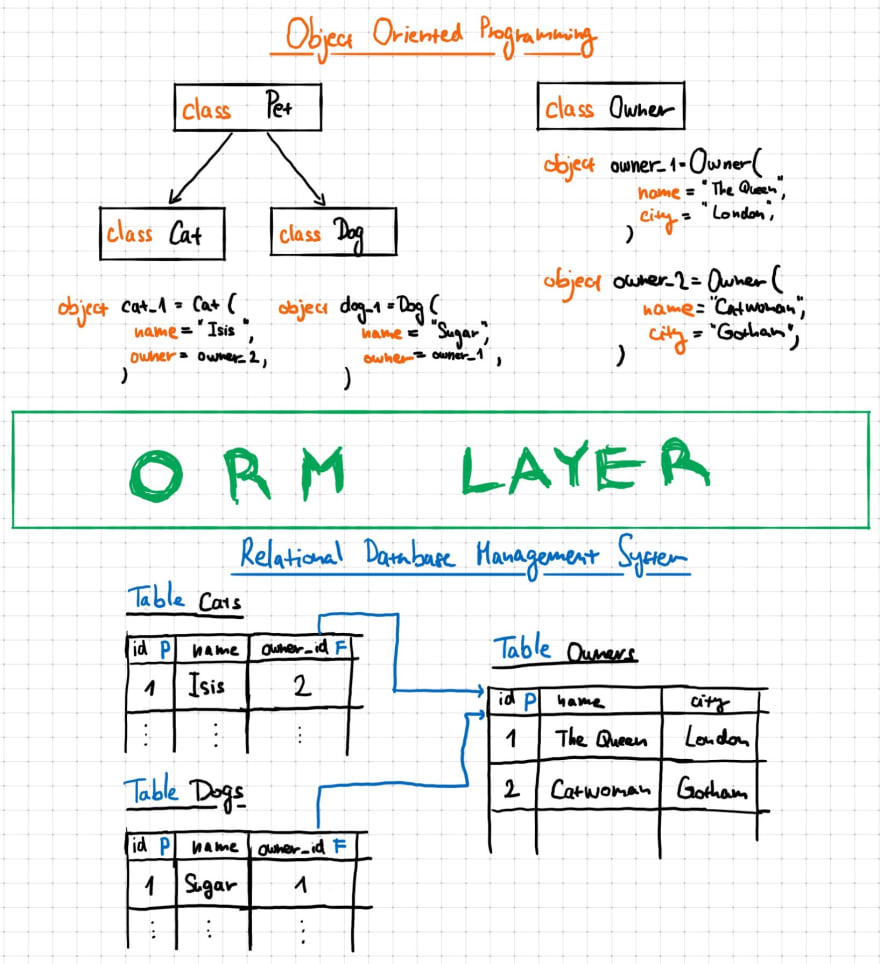
\includegraphics[width=\textwidth]{./images/chapter6/orm}


\section{What is JPA?}

The Java Persistence API (JPA; recently renamed to Jakarta Persistence API) is a specification that defines how to persist data in Java applications. JPA mainly focuses on the ORM layer and managing persistent objects.

JPA is a specification which means JPA consists of implementation guidelines for the Java ORM layer and the syntax. The specification only comes with interfaces, no actual implementation.  A reference implementation can be provided but other companies can create and distribute their own implementation of the specification.

\frame{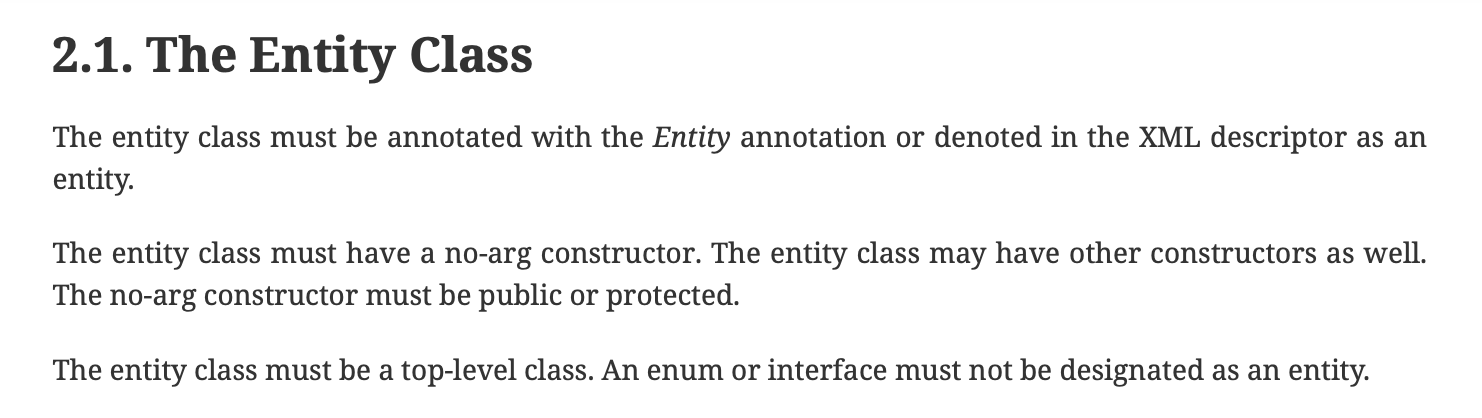
\includegraphics[width=\textwidth]{./images/chapter6/entity_class_specification}}

For our exercises and projects we will use Hibernate as the actual implementation of de JPA specification \footnote{\url{https://hibernate.org/ and https://hibernate.org/orm/}}.  

Spring Data JPA adds a layer on top of JPA. It uses all the features defined by the JPA specification, but adds no-code implementation of the repository pattern and the creation of database queries from method names.

JpaRepository extends PagingAndSortingRepository which in turn extends CrudRepository.

Their main functions are:

\begin{itemize}
\item CrudRepository mainly provides CRUD functions.
\item PagingAndSortingRepository provides methods to do pagination and sorting records.
\item JpaRepository provides some JPA-related methods such as flushing the persistence context and deleting records in a batch.
\end{itemize}


\section{Datasource}

In Spring Boot a DataSource-object is the preferred means of getting a connection to a database.
The interface jakarta.sql.DataSource is implemented by the database driver vendor. 

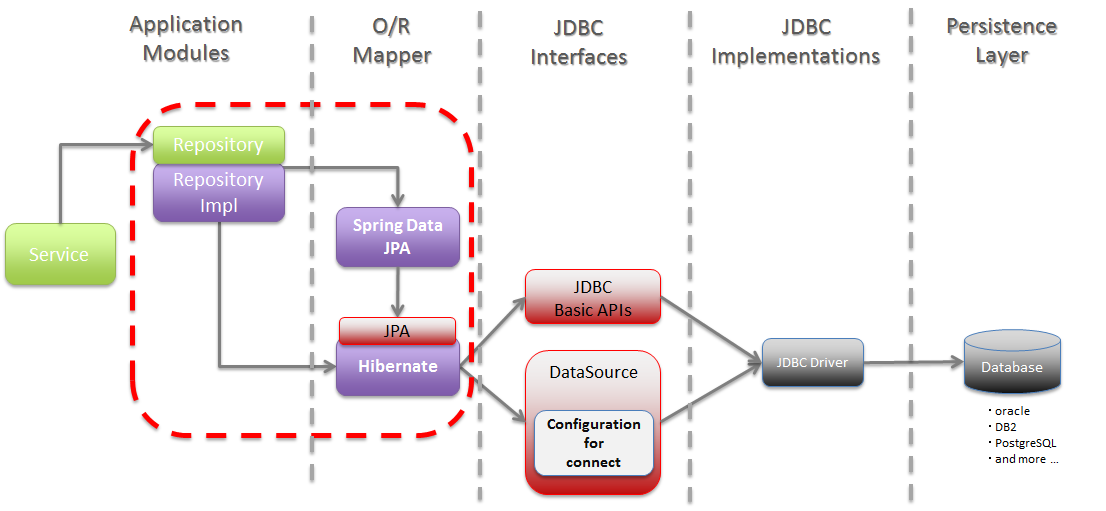
\includegraphics[width=\textwidth]{./images/chapter-jpa/springdatajpa}

The datasource can be specified in the application.properties file.
Here are some common database properties:

\begin{tabular}{|l|p{8cm}|}
\hline
spring.datasource.url & JDBC URL of the database.\\
spring.datasource.username & Login username of the database.\\
spring.datasource.password & Login password of the database.\\
spring.jpa.show-sql & Whether to enable logging of SQL statements. Default: false\\
spring.jpa.hibernate.ddl-auto & Possible values: none (production), create, create-drop, validate and update. \footnote{\url{https://stackoverflow.com/questions/42135114/how-does-spring-jpa-hibernate-ddl-auto-property-exactly-work-in-spring}}\\
\hline
\end{tabular}

Alternatively, the data source configuration can be programmatically.

The appropriate JDBC driver for your database must be included in your project. This is achieved by declaring the driver as a dependency in your project's Maven configuration file, pom.xml. The dependency ensures that the JDBC driver is available during runtime, allowing Spring Data JPA to establish and manage database connections.

Here is an example of how to include a JDBC driver for MySQL in your pom.xml file:

\begin{lstlisting}
<dependency>
<groupId>com.mysql</groupId>
<artifactId>mysql-connector-j</artifactId>
<scope>runtime</scope>
</dependency>
\end{lstlisting}

This configuration snippet includes the MySQL JDBC driver, mysql-connector-j.

Similarly,  to connect to a PostgreSQL database, you would use the PostgreSQL JDBC driver as shown below:

\begin{lstlisting}
<dependency>
<groupId>org.postgresql</groupId>
<artifactId>postgresql</artifactId>
<scope>runtime</scope>
</dependency>
\end{lstlisting}

Adjusting the driver version in your pom.xml may be necessary as you upgrade your database server or migrate to a newer version of Spring Data JPA.

\section{The Entity class}

\begin{lstlisting}[frame=single,language=java]
import jakarta.persistence.Entity;
import jakarta.persistence.Table;
import jakarta.persistence.Column;
import jakarta.persistence.Id;
import jakarta.persistence.GeneratedValue;
import jakarta.persistence.GenerationType;
import jakarta.persistence.Embedded;
import jakarta.persistence.Embeddable;

@Entity
@Table(name = "events")
public class Event {

    @Id
    @GeneratedValue(strategy = GenerationType.IDENTITY)
    private Long id;

    @Column(name = "name", nullable = false,  length = 200)
    private String title;

    @Embedded
    private EventDetails details;

    // Constructors, getters, and setters
}

@Embeddable
class EventDetails {
    private LocalDate date;
    @Column(length = 512)
    private String location;

    // Constructors, getters, and setters
}
\end{lstlisting}

A JPA entity class is a POJO (Plain Old Java Object) class  that is annotated as having the ability to represent objects in the database.
The \textbf{@Entity} annotation is used to declare that a class is an entity, so JPA will manage it and map it to a database table.

\textbf{@Table} specifies the table in the database with which the entity is mapped.

The \textbf{@Id} annotation marks a field as a primary key field.

The \textbf{@GeneratedValue} annotation is used to configure the primary key generation strategy for an entity. This annotation is usually combined with @Id to specify that the persistence provider should automatically generate a unique identifier for the entity objects. There are several strategies defined in the GenerationType enumeration that can be used with @GeneratedValue. Here's an overview:

\begin{itemize}
\item \textbf{GenerationType.AUTO}

This is the default strategy and the persistence provider will choose the generation strategy based on the specific database capabilities and dialect. 

\item \textbf{GenerationType.IDENTITY}

Indicates that the persistence provider must assign primary keys using the database identity column. This is typically supported by SQL databases with an auto-increment column.

\item \textbf{GenerationType.SEQUENCE}

Specifies that the primary key values will be generated using a database sequence. This is a special database object that generates numbers in sequential order. Not all databases support sequences.
This strategy is useful for databases supporting sequences, like Oracle, PostgreSQL, etc. It's beneficial for high-volume applications due to better performance compared to IDENTITY, as the sequence generation can be more efficiently managed.

\item \textbf{GenerationType.TABLE}

Uses a database table to simulate a sequence. This strategy uses a table to hold the next id incrementally. It's a portable solution but not as efficient as using database-specific features like sequences or identity columns.
\end{itemize}

The \textbf{@Column} annotation is used to specify the details of the column to which a field or property will be mapped. You can use column annotation with the following most commonly used attributes:
\begin{itemize}
\item \textbf{name}: specify the name of the column.
\item \textbf{length}: specify the size of thee column, particularly for a String value.
\item \textbf{nullable}: mark the column to be NOT NULL when the database schema is generated.
\item \textbf{unique}: mark the column to contain only unique values.
\end{itemize}


The \textbf{@Embeddable} annotation marks a class to be embedded within another entity.
In this example,  the EventDetails does not need its own table; instead, its properties are incorporated into the table of the entity that embeds it.

The annotation \textbf{@Embedded}  is used to denote a class whose instances are stored as an intrinsic part of an owning entity.
 All the fields of EventDetails class are embedded within the events table, avoiding the need for a separate table.


\section{Entity lifecycle}

The EntityManager is a core interface of JPA.  An instance of EntityManager is used to create and remove  entity instances, to find entities by their primary key,  and to query over entities.  In fact,  an instance of the EntityManager is used to interact with the persistence context. 

The persistence context is one of the main concepts in JPA.
It is a set of all entity object that you are currently using or used recently. You can think of the persistence context as some kind of first-level cache. Each entity object in the persistence context represents a record in the database.
The persistence context manages these entity objects and their lifecycle. Each entity object has one of 4 states: new, managed, removed, and detached.

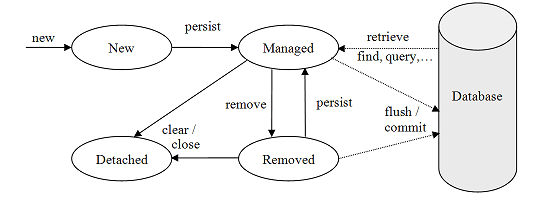
\includegraphics[width=\textwidth]{./images/chapter6/entity_states}

A newly instantiated entity object is in state \textbf{new} or \textbf{transient}. The entity object hasn't been persisted yet, so there's no database record yet. The persistence context does not know about the entity object yet. 

All entity objects that attached to the persistence context are in the lifecycle state \textbf{managed}. An entity object becomes managed when it is persisted to the database. Entity object retrieved from the database are also in the managed state.
If a managed entity object is modified (updated) within an active transaction, the change is detected by the persistence context and passed on to the database.

When a managed entity is removed within an active transaction, the state changes from managed to removed, and the record is physically deleted from the database (when the transaction commits).

An entity gets detached when it is no longer managed by the persistence context but still represents a record in the database.
Detached objects are limited in functionality.

 
Programmatically we need to use the entitymanager to change the state of the entity object in the persistence context which results in changes or updates in our database. 

When using Spring Data JPA you don't have to implement the interaction with the entitymanager. When you create a Repository, the SimpleJpaRepository class provided by Spring Data JPA provides the default implementation. SimpleJpaRepository class internally uses JPA entitymanager.

\begin{oefening}
Open the class SimpleJpaRepository and take a look at its implementation (e.g. save()-method).
\end{oefening}


\section{Relationships}

\subsection{OneToOne relationship}

A OneToOne relationship in JPA is used when one entity instance is associated with exactly one instance of another entity.  In this example a user has exactly one passport.

In a \textbf{uni-directional} OneToOne relationship, only one side of the relationship maintains knowledge of the other side’s existence. Consider a scenario where each Person has exactly one Passport. The Person entity holds a reference to the Passport, but the Passport does not hold any reference to the Person.

\begin{lstlisting}
@Entity
public class Person {
    @Id
    @GeneratedValue(strategy = GenerationType.IDENTITY)
    private Long id;
    
    @OneToOne(cascade = CascadeType.ALL)
    @JoinColumn(name = "passport_id", referencedColumnName = "id")
    private Passport passport;

    // Standard getters and setters
}

@Entity
public class Passport {
    @Id
    @GeneratedValue(strategy = GenerationType.IDENTITY)
    private Long id;
    
    private String number;

    // Standard getters and setters
}
\end{lstlisting}

In this example, the Person entity contains a Passport field annotated with @OneToOne. The @JoinColumn annotation specifies the column in the Person table that joins to the primary key of the Passport entity.

The concept of \"cascade types\" defines how persistence operations such as save, delete, and update performed on one entity should be propagated (or cascaded) to its associated entity. 

When using the @OneToOne annotation in JPA, you can specify a cascade type to automate the persistence lifecycle management of the associated entity. Here are the most common cascade types used in JPA:

\begin{itemize}
\item \textbf{CascadeType.PERSIST}: When persisting an entity, also persist the associated entity.  For example, when saving a Person object, also save its associated Passport.

\item \textbf{CascadeType.MERGE}: When merging the state of an entity into the current persistence context, also merge the entity held in this field.

\item \textbf{CascadeType.REMOVE}: When deleting an entity, also delete the associated entity. This is particularly useful when the associated entity no longer makes sense to exist independently.

\item \textbf{CascadeType.REFRESH}: When refreshing an entity, also refresh the entities held in this field. This means reloading the content of the associated entity from the database, which can be useful if the database might be changed by other processes.

\item \textbf{CascadeType.DETACH}: When an entity is detached from the persistence context, also detach the entities held in this field.

\item \textbf{CascadeType.ALL}: A convenience that cascades all the above operations (PERSIST, MERGE, REMOVE, REFRESH, DETACH). Using CascadeType.ALL is common for @OneToOne and @OneToMany associations.
\end{itemize}

In a \textbf{bi-directional} OneToOne relationship, both entities are aware of each other. This relationship allows navigation from either side. Using the same example as above, both the Person and Passport entities can have references to each other.

\begin{lstlisting}
@Entity
public class Person {
    @Id
    @GeneratedValue(strategy = GenerationType.IDENTITY)
    private Long id;

    @OneToOne(mappedBy = "person", cascade = CascadeType.ALL)
    private Passport passport;

    // Standard getters and setters
}

@Entity
public class Passport {
    @Id
    @GeneratedValue(strategy = GenerationType.IDENTITY)
    private Long id;

    private String number;

    @OneToOne
    @JoinColumn(name = "person_id")
    private Person person;

    // Standard getters and setters
}
\end{lstlisting}

In this bi-directional setup, the Person entity uses the mappedBy attribute in the @OneToOne annotation to indicate that the Person is not the owner of the relationship and that the Passport entity contains the foreign key.

\subsection{ManyToOne relationship}

A ManyToOne relationship in JPA is commonly used when one entity is related to multiple instances of another entity. For instance, in a blog system, many posts may belong to one category.

Uni-directional ManyToOne Relationship
In a uni-directional ManyToOne relationship, only the 'many' side of the relationship is aware of the 'one' side. This setup is often seen when the 'one' side doesn't need to directly access the 'many' side.

Example: Books and Authors
Suppose each book can have one author, but each author can write many books. Here, the relationship from books to authors is a typical example of a uni-directional ManyToOne relationship.

\begin{lstlisting}
@Entity
public class Book {
    @Id
    @GeneratedValue(strategy = GenerationType.IDENTITY)
    private Long id;

    private String title;

    @ManyToOne
    @JoinColumn(name = "author_id", nullable = false)
    private Author author;

    // Standard getters and setters
}

@Entity
public class Author {
    @Id
    @GeneratedValue(strategy = GenerationType.IDENTITY)
    private Long id;

    private String name;

    // Standard getters and setters, no reference back to Book
}
\end{lstlisting}

In this model, each Book entity holds a reference to its Author, which is annotated with @ManyToOne. The @JoinColumn annotation specifies the foreign key column in the Book table that links to the Author.

Repository Configuration
Repositories for each entity can be defined as follows:

\begin{lstlisting}
public interface BookRepository extends JpaRepository<Book, Long> {
}

public interface AuthorRepository extends JpaRepository<Author, Long> {
}
\end{lstlisting}

Bi-directional ManyToOne Relationship
In a bi-directional relationship, both sides of the relationship are aware of each other. This is useful when you want to navigate the relationship from either side.

Example: Books and Authors Continued
Expanding on the previous example, suppose now we want authors to also be aware of the books they've written.

Entity Definition
\begin{lstlisting}
@Entity
public class Book {
    @Id
    @GeneratedValue(strategy = GenerationType.IDENTITY)
    private Long id;

    private String title;

    @ManyToOne
    @JoinColumn(name = "author_id", nullable = false)
    private Author author;

    // Standard getters and setters
}

@Entity
public class Author {
    @Id
    @GeneratedValue(strategy = GenerationType.IDENTITY)
    private Long id;

    private String name;

    @OneToMany(mappedBy = "author")
    private Set<Book> books = new HashSet<>();

    // Standard getters and setters
}
\end{lstlisting}

In this bi-directional setup, the Author class includes a Set<Book> to hold the collection of books. The @OneToMany annotation in Author uses the mappedBy attribute to indicate that the Author entity is not the owner of the relationship and that the Book entity contains the foreign key.

\subsection{ManyToMany relationship}


A ManyToMany relationship is used when multiple instances of one entity are associated with multiple instances of another entity. Using the example of books and authors, a ManyToMany relationship would be appropriate if each book could have multiple authors and each author could write multiple books. 

In a uni-directional ManyToMany relationship, only one entity maintains the relationship information.

Imagine a scenario where each book can have multiple authors, but we are only interested in navigating from books to authors and not the other way around.

\begin{lstlisting}
@Entity
public class Book {
    @Id
    @GeneratedValue(strategy = GenerationType.IDENTITY)
    private Long id;

    private String title;

    @ManyToMany
    @JoinTable(
        name = "book_author",
        joinColumns = @JoinColumn(name = "book_id"),
        inverseJoinColumns = @JoinColumn(name = "author_id")
    )
    private Set<Author> authors = new HashSet<>();

    // Standard getters and setters
}

@Entity
public class Author {
    @Id
    @GeneratedValue(strategy = GenerationType.IDENTITY)
    private Long id;

    private String name;

    // Standard getters and setters, no reference back to Books
}
\end{lstlisting}
In this example, the Book entity defines a ManyToMany relationship to the Author entity. The @JoinTable annotation specifies the table that maps books to authors, including columns for each foreign key.


In a bi-directional ManyToMany relationship, both entities are aware of each other, and navigation is possible from either side.

This time, both books and authors are aware of each other and can navigate the relationship.

\begin{lstlisting}
@Entity
public class Book {
    @Id
    @GeneratedValue(strategy = GenerationType.IDENTITY)
    private Long id;

    private String title;

    @ManyToMany
    @JoinTable(
        name = "book_author",
        joinColumns = @JoinColumn(name = "book_id"),
        inverseJoinColumns = @JoinColumn(name = "author_id")
    )
    private Set<Author> authors = new HashSet<>();

    // Standard getters and setters
}

@Entity
public class Author {
    @Id
    @GeneratedValue(strategy = GenerationType.IDENTITY)
    private Long id;

    private String name;

    @ManyToMany(mappedBy = "authors")
    private Set<Book> books = new HashSet<>();

    // Standard getters and setters
}
\end{lstlisting}

In the bi-directional arrangement, the Author entity includes a Set<Book> to hold the collection of books. The mappedBy attribute indicates that the Author is not the owner of the relationship, and the mapping details are managed by the Book entity.

\section{Fetching strategy}

JPA provides two main fetching strategies to control how related entities are loaded from the database:

\begin{itemize}
\item \textbf{Eager Fetching}: With eager fetching, related entities are loaded immediately with the main entity, whether they are accessed in the application or not. This can lead to performance issues if the relationships involve large sets of data. Eager fetching is often used when the data sets are small or always used together with the main entity.

\item \textbf{Lazy Fetching}: Lazy fetching loads the related entities only when they are explicitly accessed in the application. This can improve performance by reducing the initial load time and the amount of memory consumed. However, it requires careful management of the persistence context to avoid LazyInitializationException.
\end{itemize}

java
Copy code
@ManyToMany(fetch = FetchType.LAZY)
private Set<Author> authors = new HashSet<>();
In the case of ManyToMany relationships, the default fetching strategy is lazy because eager fetching can result in very large numbers of joins and thus severe performance degradation.

Understanding and choosing the right fetching strategy based on the specific use case and data access patterns is crucial for developing efficient, scalable applications.

Consider the following method findBooksByAuthor() in a BookService.
When we look closely at the logging of the SQL-queries. We see that first, the author is retrieved and later, the author's books are retrieved on the moment we call author.getBooks(), not sooner. This is lazy loading or lazy fetching. When dealing with one-to-many or many-to-many relationships, lazy fetching is mostly the best solution in terms of performance.

\begin{lstlisting}
@Service
public class BookService {

    private static final Logger LOGGER = LogManager.getLogger(BookService.class);

    private final AuthorRepository authorRepository;

    public BookService(AuthorRepository authorRepository) {
        this.authorRepository = authorRepository;
    }

    public List<String> getBooksByAuthor(String authorName) {
        Author author = authorRepository.findAuthorByName(authorName).orElseThrow(() -> new NotFoundException("No author found"));
        LOGGER.info("Author retrieved...");
        return author.getBooks().stream().map(Book::getTitle).toList();
    }
}
\end{lstlisting}

\begin{verbatim}
2024-04-23T20:23:48.883+02:00  INFO 26656 --- [nio-8080-exec-8] be.pxl.helpdesk.service.BookService      : Starting getBooksByAuthor
Hibernate: 
    select
        a1_0.id,
        a1_0.name 
    from
        authors a1_0 
    where
        a1_0.name=?
2024-04-23T20:23:48.946+02:00  INFO 26656 --- [nio-8080-exec-8] be.pxl.helpdesk.service.BookService      : Author retrieved...
Hibernate: 
    select
        b1_0.author_id,
        b1_1.id,
        b1_1.title 
    from
        book_authors b1_0 
    join
        books b1_1 
            on b1_1.id=b1_0.book_id 
    where
        b1_0.author_id=?
\end{verbatim}

If we change the relationship between Author and Books to eager fetching, the books are retrieved on the moment we search the author by its name.


\begin{lstlisting}
@Entity
@Table(name = "authors")
public class Author {
    @Id
    @GeneratedValue(strategy = GenerationType.IDENTITY)
    private Long id;

    private String name;

    @ManyToMany(mappedBy = "authors", fetch = FetchType.EAGER)
    private Set<Book> books = new HashSet<>();

    // Standard getters and setters

    public void addBook(Book book) {
        books.add(book);
    }

    public Set<Book> getBooks() {
        return books;
    }
}
\end{lstlisting}

\begin{verbatim}
2024-04-23T20:21:02.145+02:00  INFO 19956 --- [nio-8080-exec-6] be.pxl.helpdesk.service.BookService      : Starting getBooksByAuthor
Hibernate: 
    select
        a1_0.id,
        a1_0.name 
    from
        authors a1_0 
    where
        a1_0.name=?
Hibernate: 
    select
        b1_0.author_id,
        b1_1.id,
        b1_1.title 
    from
        book_authors b1_0 
    join
        books b1_1 
            on b1_1.id=b1_0.book_id 
    where
        b1_0.author_id=?
2024-04-23T20:21:02.216+02:00  INFO 19956 --- [nio-8080-exec-6] be.pxl.helpdesk.service.BookService      : Author retrieved...
\end{verbatim}

Always be very carefull with bi-directional relationships and eager fetching. The performance cost may be underestimated. In this case, if an author has written many books, it may be beneficial, to only maintain the owning part of the relationship and search for in author's books with a query in the BookRepository.

\section{Transactions}

The @Transactional Annotation in Spring Boot
The @Transactional annotation in Spring Boot is used to declare that a method or a class should be executed within a transactional context. This is a powerful feature provided by the Spring Framework that manages the transaction management boilerplate that can complicate the application code and ensures that your transaction requirements are handled consistently.

Key Concepts:
Transaction: A sequence of actions that are treated as a single unit of work. These actions should either complete entirely or take no effect at all.
Transaction Management: Ensures that an application maintains data integrity and consistency in scenarios involving multiple transaction operations.
Usage of @Transactional
At the method level: When placed above a method, @Transactional ensures the method executes within a transaction. If a transaction is already running, the method by default runs within that transaction.
At the class level: If @Transactional is placed at the class level, it applies to all the public methods of that class.
Transaction Propagation
Transaction propagation behavior defines how transactions relate to each other. Common propagation types include:

REQUIRED: Use the current transaction or start a new one if none exists.
REQUIRES\_NEW: Always start a new transaction, suspending the current one if it exists.
SUPPORTS: Run within the current transaction if it exists; otherwise, run non-transactionally.
NEVER: Ensure no current transaction exists, throwing an exception if one exists.
Flowchart of How Transactions Work in Spring Boot
Here’s a simplified flowchart illustrating how transactions are managed in Spring Boot using the @Transactional annotation:

Method Invocation: A method annotated with @Transactional is called.
Check Existing Transaction: The transaction manager checks if a current transaction exists.
Transaction Propagation: Depending on the propagation setting:
Use current transaction or start a new one.
Suspend the current transaction and start a new one.
Run without a transaction if none exists.
Method Execution: The method executes. Database operations are performed as part of the transaction.
Commit/Rollback:
If the method completes successfully, the transaction is committed.
If an exception occurs, the transaction is rolled back.
Example: Book and Author Entities
Let’s consider an example with Book and Author entities. We want to ensure that adding a book linked to an author is transactional (either both the book and the author are saved, or neither).

Entity Classes
java
Copy code
@Entity
public class Author {
    @Id
    @GeneratedValue(strategy = GenerationType.AUTO)
    private Long id;
    private String name;
    // constructors, getters, and setters
}

@Entity
public class Book {
    @Id
    @GeneratedValue(strategy = GenerationType.AUTO)
    private Long id;
    private String title;
    @ManyToOne
    private Author author;
    // constructors, getters, and setters
}
Service Class with Transactional Methods
java
Copy code
@Service
public class LibraryService {
    @Autowired
    private BookRepository bookRepository;
    @Autowired
    private AuthorRepository authorRepository;

    @Transactional
    public void addBookAndAuthor(Book book, Author author) {
        authorRepository.save(author); // Save author
        book.setAuthor(author);
        bookRepository.save(book); // Save book
        // Both saves are part of the same transaction
    }
}

\section{Queries}

Basic CRUD queries are in Spring Data JPA available in the repositories. But there are multiple ways of creating custom queries in a Spring boot application. Let's discuss the different
types of queries.

\subsection{Query methods}

Spring Data JPA can create queries based on method names. You can use keywords like \textit{findBy}, \textit{findAllBy},
\textit{findBy...And...}, ...

An overview of the keywords can be found in spring documentation \url{https://docs.spring.io/spring-data/jpa/reference/jpa/query-methods.html}.

\begin{lstlisting}
public interface ProductRepository extends JpaRepository<Product, Long> {
    // Query method with parameters for finding products by name and price
    List<Product> findByNameAndPrice(String name, double price);
}
\end{lstlisting}

\subsection{JPQL queries}

JPQL, or Java Persistence Query Language, is a query language designed to abstract database details from the developer, allowing queries to be written based on entity model classes rather than on database tables.


\begin{lstlisting}
public interface UserRepository extends JpaRepository<User, Long> {
  @Query("SELECT u FROM User u WHERE u.age >= :minAge")
  List<User> findByAgeGreaterThan(@Param("minAge") int minAge);
}
\end{lstlisting}

\subsection{Native SQL queries}

\begin{lstlisting}

\end{lstlisting}


\section{Unit testing a repository}

Spring Data JPA offers an annotation @DataJpaTest which makes repository testing possible with a minimum of configuration. 

Add the h2 dependency with scope test in your pom.xml. This way the unit test for your repository will use the h2 database to test your queries.

\begin{lstlisting}
<dependency>
	<groupId>com.h2database</groupId>
	<artifactId>h2</artifactId>
	<scope>test</scope>
</dependency>
\end{lstlisting}

The builder pattern is used in this example to create entity objects for testing purpose. These entity objects are stored in the in-memory database. There is an IntelliJ IDEA plugin that generates the builder-classes for you (Generate Builder plugin).

\begin{lstlisting}
public final class AuthorBuilder {
    private String name;
    private Set<Book> books;

    private AuthorBuilder() {
    }

    public static AuthorBuilder anAuthor() {
        return new AuthorBuilder();
    }

    public AuthorBuilder withName(String name) {
        this.name = name;
        return this;
    }

    public AuthorBuilder withBooks(Set<Book> books) {
        this.books = books;
        return this;
    }

    public Author build() {
        Author author = new Author();
        author.setName(name);
        author.setBooks(books);
        return author;
    }
}
\end{lstlisting}

The @DataJpaTest annotation is used to test JPA repositories in Spring Boot applications. It’s a specialized test annotation that provides a minimal Spring context for testing the persistence layer. 

By default, each test method annotated with @DataJpaTest runs within a transactional boundary. This ensures that changes made to the database are automatically rolled back at the end of the test, leaving a clean slate for the next test.

The test class uses the entity managers, which is injected in the test with the @PersistenceContext annotation. The flush() forces to synchronize the persistence context to the database. The clear() empties the persistence context. Therefore, all entities are detached and can be fetched from the database.


\begin{lstlisting}[frame=single, language=java]
package be.pxl.helpdesk.repository;

import be.pxl.helpdesk.builder.AuthorBuilder;
import be.pxl.helpdesk.domain.Author;
import jakarta.persistence.EntityManager;
import jakarta.persistence.PersistenceContext;
import org.junit.jupiter.api.BeforeEach;
import org.junit.jupiter.api.Test;
import org.springframework.beans.factory.annotation.Autowired;
import org.springframework.boot.test.autoconfigure.orm.jpa.DataJpaTest;

import java.util.Arrays;
import java.util.Optional;

import static org.junit.jupiter.api.Assertions.assertEquals;
import static org.junit.jupiter.api.Assertions.assertTrue;

@DataJpaTest
public class AuthorRepositoryTest {

	@PersistenceContext
	protected EntityManager entityManager;

	@Autowired
	private AuthorRepository authorRepository;

	private final Author author1 = AuthorBuilder.anAuthor().withName("Famous Author").build();


	private final Author author2 = AuthorBuilder.anAuthor().withName("Not So Famous Author").build();

	@BeforeEach
	public void init() {
		authorRepository.saveAll(Arrays.asList(author1, author2));
		entityManager.flush();
		entityManager.clear();
	}

	@Test
	public void returnsAuthorByName() {
		Optional<Author> author = authorRepository.findAuthorByName("Famous Author");

		assertTrue(author.isPresent());
		assertEquals("Famous Author", author.get().getName());
	}

	@Test
	public void returnsEmptyOptionalWhenNoAuthorPlayerWithName() {
		Optional<Author> author = authorRepository.findAuthorByName("Bestseller Author");

		assertTrue(author.isEmpty());
	}
}
\end{lstlisting}


\section{Pagination}

Pageable is an interface provided by Spring Data that contains information about the pagination and sorting of data. It helps in structuring the way data is retrieved from the database in manageable chunks or pages, rather than pulling large quantities of data all at once, which can be inefficient and slow.


\begin{lstlisting}
@RestController
@RequestMapping("books")
public class BookController {

    private final BookService bookService;

    public BookController(BookService bookService) {
        this.bookService = bookService;
    }

    @GetMapping("search")
    public List<BookDto> searchBooks(@RequestBody FilterDto filter) {
        return bookService.searchBooks(filter);
    }

    @GetMapping
    public Page<BookDto> getBooks(Pageable pageable) {
        return bookService.findAllBooks(pageable);
    }
}
\end{lstlisting}

The parameter Pageable is automatically populated by Spring when the method is called. The Pageable object typically includes:
\begin{itemize}
\item page: The current page number (0-indexed, where 0 is the first page).
\item size: The number of records per page.
\item sort: Criteria for sorting the data (optional).
\end{itemize}

For example, a request URL might look like this: \textit{/books?page=0\&size=10\&sort=title,asc}. This tells the application to get the first page of books, with 10 books per page, sorted by title in ascending order.

\begin{lstlisting}
@Service
public class BookService {

    private static final Logger LOGGER = LogManager.getLogger(BookService.class);

    private final AuthorRepository authorRepository;
    private final BookRepository bookRepository;

    public BookService(AuthorRepository authorRepository, BookRepository bookRepository) {
        this.authorRepository = authorRepository;
        this.bookRepository = bookRepository;
    }

    public List<String> getBooksByAuthor(String authorName) {
        LOGGER.info("Starting getBooksByAuthor");
        Author author = authorRepository.findAuthorByName(authorName).orElseThrow(() -> new NotFoundException(""));
        LOGGER.info("Author retrieved...");
        return author.getBooks().stream().map(Book::getTitle).toList();
    }

    public Page<BookDto> findAllBooks(Pageable pageable) {
        Page<Book> books = bookRepository.findAll(pageable);
        return books.map(this::mapToBookDto);
    }


    private BookDto mapToBookDto(Book book) {
        return new BookDto(book.getTitle(), book.getCategory(), book.getAuthors().stream().map(Author::getName).toList());
    }
}
\end{lstlisting}

The Pageable parameter is passed to the bookService.findAllBooks(pageable) method. This method is expected to interact with the repository layer that extends Spring Data’s PagingAndSortingRepository or JpaRepository. These repositories natively support Pageable for pagination and sorting.
The repository method would use the Pageable object to construct a database query that fetches only the specified slice of data based on the page number, page size, and sorting criteria.
Return Type (Page<BookDto>):
The method returns a Page<BookDto>, which is a specialized implementation of the Slice interface. It provides not only the list of data for the current page but also additional information about the total number of pages, the total number of elements, whether there are more pages available, and so forth.
Benefits of Using Pageable
Efficiency: Only the necessary slice of data is fetched from the database, which can be crucial for performance when dealing with large datasets.
Flexibility: Clients of your API can specify how many records they want per page and how the data should be sorted.
Ease of Use: Spring Data handles much of the heavy lifting, making it easier to implement robust pagination and sorting without much boilerplate code.


\begin{lstlisting}

\end{lstlisting}

\begin{verbatim}
{
	"content": [
		{
			"title": "Whispers of the Ancient",
			"category": null,
			"authors": [
				"Tessa Fairwind",
				"Elara Thornwood"
			]
		},
		{
			"title": "The Last Ember",
			"category": null,
			"authors": [
				"Milo Ventris"
			]
		},
		{
			"title": "Beneath the Starless Sky",
			"category": null,
			"authors": [
				"Tessa Fairwind"
			]
		},
		{
			"title": "Echoes of the Forgotten",
			"category": null,
			"authors": [
				"Quentin Ashlore"
			]
		},
		{
			"title": "The Glass Fortress",
			"category": null,
			"authors": [
				"Nora Spellbound",
				"Quentin Ashlore"
			]
		}
	],
	"pageable": {
		"pageNumber": 0,
		"pageSize": 5,
		"sort": {
			"empty": true,
			"sorted": false,
			"unsorted": true
		},
		"offset": 0,
		"paged": true,
		"unpaged": false
	},
	"last": false,
	"totalPages": 2,
	"totalElements": 10,
	"size": 5,
	"number": 0,
	"sort": {
		"empty": true,
		"sorted": false,
		"unsorted": true
	},
	"numberOfElements": 5,
	"first": true,
	"empty": false
}
\end{verbatim}

\section{Searching and filtering data}







\chapter{Mockito}

\fcolorbox{black}[HTML]{E9F0E9}{\parbox{\textwidth}{%
\noindent \textbf{Learning goals}\\
The junior-colleague
\begin{enumerate}[nolistsep]
\item can describe the usage of mockito.
\item can implement unit tests with mockito.
\end{enumerate}}}

\section{Mocking with Mockito}

Mockito is a popular open source framework for mocking objects in software test.

\begin{lstlisting}
package be.pxl.superhero.service;

public class MyService {

    private final OtherService otherService;

    public MyService(OtherService otherService) {
        this.otherService = otherService;
    }

    public int doCalculation(int value) {
        return value * otherService.getValue();
    }
}
\end{lstlisting}

\begin{lstlisting}
package be.pxl.superhero.service;

public interface OtherService {

    int getValue();
}
\end{lstlisting}

When writing a unit test for the method doCalculation() we need an object of the class OtherService. We don't need an object of an actual implementation of the interface. We can just mock the OtherService-object and tell it what it should return when it's called.

\begin{lstlisting}
package be.pxl.superhero.service;

import org.junit.jupiter.api.Test;
import org.junit.jupiter.api.extension.ExtendWith;
import org.mockito.InjectMocks;
import org.mockito.Mock;
import org.mockito.junit.jupiter.MockitoExtension;

import static org.junit.jupiter.api.Assertions.assertEquals;
import static org.mockito.Mockito.when;

@ExtendWith(MockitoExtension.class)
public class MyServiceTest {

    @Mock
    private OtherService otherService;
    @InjectMocks
    private MyService myService;

    @Test
    public void doCalculationTest() {
        when(otherService.getValue()).thenReturn(5);
        assertEquals(500, myService.doCalculation(100));
    }
}
\end{lstlisting}

\section{Unit testing the service-layer methods}


We use Mockito when we test the Service-layer of an application. In this section we discuss more complex unit tests with Mockito.

The name of a superhero must be unique. To accomplish this, we add the unique constraint to our database column. 
However, it is good practice to implement this business rule in the service layer.
Database constraints are the last line of defence, not the only. 


\begin{lstlisting}[frame=single, language=java]
package be.pxl.superhero.service.impl;

import be.pxl.superhero.api.MissionDTO;
import be.pxl.superhero.api.SuperheroDTO;
import be.pxl.superhero.api.SuperheroDetailDTO;
import be.pxl.superhero.api.SuperheroRequest;
import be.pxl.superhero.domain.Mission;
import be.pxl.superhero.domain.Superhero;
import be.pxl.superhero.exception.ResourceNotFoundException;
import be.pxl.superhero.repository.MissionRepository;
import be.pxl.superhero.repository.SuperheroRepository;
import be.pxl.superhero.service.SuperheroService;
import jakarta.validation.ValidationException;
import org.springframework.stereotype.Service;
import org.springframework.transaction.annotation.Transactional;

import java.util.List;
import java.util.Optional;

@Service
public class SuperheroServiceImpl implements SuperheroService {

    private final SuperheroRepository superheroRepository;
    private final MissionRepository missionRepository;

    public SuperheroServiceImpl(SuperheroRepository superheroRepository,
                                MissionRepository missionRepository) {
        this.superheroRepository = superheroRepository;
        this.missionRepository = missionRepository;
    }

    public Long createSuperhero(SuperheroRequest superheroRequest) {
        Optional<Superhero> existingSuperhero = 
            superheroRepository.findSuperheroBySuperheroName(superheroRequest.getSuperheroName());
        existingSuperhero.ifPresent(s -> {
            throw new ValidationException("This superhero name is already taken.");
        });
            
        Superhero superhero = new Superhero();
        superhero.setFirstName(superheroRequest.firstName());
        superhero.setLastName(superheroRequest.lastName());
        superhero.setSuperheroName(superheroRequest.superheroName());
        Superhero newSuperhero = superheroRepository.save(superhero);
        return newSuperhero.getId();
    }

    // other methods intentionally left out
}
\end{lstlisting}


Now we need unit tests for the method \textit{createSuperhero}. There's one problem, we need a SuperheroRepository to thoroughly test the method.  The solution is to mock the database layer. Here,  mocking means create a dummy layer and no actual database operation will be executed. 

In Mockito we can mock methods in 2 different ways:

\begin{itemize}
\item Using when-then syntax e.g.: when(..).thenReturn() or when(..).thenAnswer(…)
\item Using do-when syntax e.g.: doReturn(..).when()
\end{itemize}

For mocked objects it is best practice to use when-then option as it provides return type checking and it is more readable.

For mocking void methods, there is no when-then option. We have to use do-when syntax.

\begin{lstlisting}[frame=single, language=java]
package be.pxl.superhero.service.impl;

import be.pxl.superhero.api.SuperheroDTO;
import be.pxl.superhero.api.SuperheroRequest;
import be.pxl.superhero.builder.SuperheroBuilder;
import be.pxl.superhero.domain.Superhero;
import be.pxl.superhero.repository.SuperheroRepository;
import jakarta.validation.ValidationException;
import org.junit.jupiter.api.Test;
import org.junit.jupiter.api.extension.ExtendWith;
import org.mockito.*;
import org.mockito.junit.jupiter.MockitoExtension;

import java.util.Arrays;
import java.util.List;
import java.util.Optional;
import java.util.stream.Collectors;

import static org.assertj.core.api.Assertions.assertThat;
import static org.junit.jupiter.api.Assertions.assertEquals;
import static org.junit.jupiter.api.Assertions.assertThrows;
import static org.mockito.Mockito.when;

@ExtendWith(MockitoExtension.class)
public class SuperheroServiceImplTest {

	private static final String SUPERHERO_NAME = "Superman";
	private static final String FIRST_NAME = "Clark";
	private static final String LAST_NAME = "Kent";
	private static final long SUPERHERO_ID = 115;

	@Mock
	private SuperheroRepository superheroRepository;
	@Mock
	private Superhero newSuperhero;

	@Captor
	private ArgumentCaptor<Superhero> superheroCaptor;

	@InjectMocks
	private SuperheroServiceImpl superheroService;

	private final Superhero superhero = SuperheroBuilder.aSuperhero()
			.withFirstName(FIRST_NAME)
			.withLastName(LAST_NAME)
			.withSuperheroName(SUPERHERO_NAME)
			.build();

	@Test
	public void throwsValidationExceptionWhenSuperheroNameIsNotUnique() {
		when(superheroRepository.findSuperheroBySuperheroName(SUPERHERO_NAME))
		    .thenReturn(Optional.of(superhero));
		SuperheroRequest request = new SuperheroRequest(FIRST_NAME, LAST_NAME, SUPERHERO_NAME);
		ValidationException validationException = assertThrows(ValidationException.class, 
		    () -> superheroService.createSuperhero(request));
		assertEquals("This superhero name is already taken.", validationException.getMessage());
	}

	@Test
	public void savesSuperheroWhenSuperheroNameIsUnique() {
		when(superheroRepository.findSuperheroBySuperheroName(SUPERHERO_NAME))
		    .thenReturn(Optional.empty());
		when(newSuperhero.getId())
		    .thenReturn(SUPERHERO_ID);
		when(superheroRepository.save(Mockito.any(Superhero.class)))
		    .thenReturn(newSuperhero);
		SuperheroRequest request = new SuperheroRequest(FIRST_NAME, LAST_NAME, SUPERHERO_NAME);
		Long newId = superheroService.createSuperhero(request);
		assertEquals(SUPERHERO_ID, newId);
		Mockito.verify(superheroRepository).save(superheroCaptor.capture());
		Superhero savedSuperhero = superheroCaptor.getValue();
		assertEquals(FIRST_NAME, savedSuperhero.getFirstName());
		assertEquals(LAST_NAME, savedSuperhero.getLastName());
		assertEquals(SUPERHERO_NAME, savedSuperhero.getSuperheroName());
	}

	@Test
	public void findAllSuperheroes() {
		Superhero hero1 = SuperheroBuilder.aSuperhero()
		                                  .withSuperheroName("Batman")
		                                  .build();
		Superhero hero2 = SuperheroBuilder.aSuperhero()
		                                  .withSuperheroName("Superman")
		                                  .build();
		when(superheroRepository.findAll()).thenReturn(Arrays.asList(hero1, hero2));
		List<SuperheroDTO> allSuperheroes = superheroService.findAllSuperheroes();
		assertThat(allSuperheroes.stream().map(SuperheroDTO::superheroName)
		                                  .collect(Collectors.toList()))
				.hasSize(2)
				.containsExactly("Batman", "Superman");
	}

}
\end{lstlisting}

All test classes that use Mockito, are annotated with @ExtendWith(MockitoExtension.class).  We want to create a dummy SuperheroRepository, therefore we create it with the annotation @Mock.
This dummy SuperheroRepsitory should be used by the SuperheroService under test.  We use the annotation @InjectMocks to use all the dummy classes in the SuperheroService instance.

The test throwsValidationExceptionWhenSuperheroNameIsNotUnique is a test for the scenario where the superhero is already saved in the database. Our dummy SuperheroRepository will return this existing superhero when he is retrieved by his superheroName.
During the test we call the method createSuperhero with test data but we expect the method to throw a ValidationException.  If the exception is not thrown, the test will fail. Finally, the error message of the exception is verified.

The test savesSuperheroWhenSuperheroNameIsUnique is a test for the scenario where the superhero doesn't exist yet.
The dummy SuperheroRepository will return an empty Optional.  While executing the test, the save method of the SuperheroRepository is called.  The result of this save method is used for creating the SuperheroDTO that is returned by the SuperheroService under test.
The save-method cannot return null, it would cause our test to end with a NullPointerException. Therefore, we make our dummy SuperheroRepository return something useful. We verify the return value of the method under test (createSuperhero). We verify the save() method is called with the expected argument.  This is accomplished with an argument captor. 

The third test is a test for the method findAllSuperheroes.  We test that the results retrieved from the dummy SuperheroRepository are mapped correctly to SuperheroDTOs.  This test uses AssertJ for the assertions. This is a useful library for writing readable assertions. 
 
\begin{oefening}
Add the class SuperheroServiceTest to your project and run (and debug!) the tests. 
Create a new test class with the name SuperheroServiceUpdateSuperheroTest.
Write unit tests for the method updateSuperhero in the class SuperheroServiceTest. 
\end{oefening}
 
 
 
 
 \section{Example of TDD}
 
 TODO::: https://learning.oreilly.com/course/master-java-unit/9781789346077/
 
 TESTING DOUBLES
 
 In general, it is a good thing to avoid tight coupling between components of the system. In line with
this rule, we want to make sure that the subscribers know as little as possible about the service, and vice
versa. To achieve this result, we can use a publish/subscribe design pattern7 which does exactly this: it
decouples publisher(s) from subscribers.
First, let us discuss some requirements for our class - RaceResultsService:
• It should allow clients to subscribe (which means they start receiving messages),
• It should allow subscribers to unsubscribe (which means they stop receiving messages),
• Every time a new message comes, it should be sent to all subscribers.
These simple requirements, along with some common sense, already furnish us with a lot of test cases.
In the ensuing sections we will be implementing the following:
• If the client is not subscribed, it should not receive any messages,
• If client is subscribed, it should receive each incoming message once (and only once),
• If multiple clients are subscribed, each of them should receive each incoming message,
• Consecutive subscribe requests issued by the same client will be ignored (nothing happens),
• If the client unsubscribes, then it should be the case that no more messages are sent to it.
We shall test RaceResultsService (the SUT) and make sure it sends messages to the right subscribers
(DOCs). At first glance, it seems like we must have at least three types to implement the discussed

from the book  practical testing (pdf)

Please enhance the Race Results example (see Section 5.4) with the following functionality:
• RaceResultsService should send messages with the results of different categories of race - e.g. horse
races, F1 races, boat-races, etc. Subscribers should be able to subscribe to selected categories. Make
sure they receive only messages related to the ones they have signed up for.
• Each message sent by RaceResultsService should be logged. Introduce a logging DOC, and make
sure that the date and text of each message is logged. Do not implement the logging mechanism:
concentrate on the interactions between the service and its collaborator.
• In the tests implemented so far, RaceResultsService sends only one message. This is unrealistic!
Enhance the tests to ensure that subscribers will receive any number of sent messages.
• What should happen if a client that is not subscribed tries to unsubscribe? Make up your mind about
it, write a test which verifies this behaviour, and make RaceResultsService behave accordingly.
 
 
 Example: Testing a Service Layer Method
Suppose you have a BookService that depends on a BookRepository. You want to test the findAllBooks() service method, which retrieves all books from the repository.

Step 1: Set Up Your Service and Repository

First, define your BookRepository and BookService interfaces:

java
Copy code
public interface BookRepository {
    List<Book> findAll();
}

@Service
public class BookService {
    private final BookRepository bookRepository;

    @Autowired
    public BookService(BookRepository bookRepository) {
        this.bookRepository = bookRepository;
    }

    public List<Book> findAllBooks() {
        return bookRepository.findAll();
    }
}
Step 2: Write the Test Class

Next, create a test class for BookService:

java
Copy code
@ExtendWith(SpringExtension.class)
public class BookServiceTest {

    @Mock
    private BookRepository bookRepository;

    @InjectMocks
    private BookService bookService;

    @Test
    public void testFindAllBooks() {
        // Arrange
        Book book1 = new Book("Book 1", "Author 1", 2019);
        Book book2 = new Book("Book 2", "Author 2", 2020);
        List<Book> mockBooks = Arrays.asList(book1, book2);
        Mockito.when(bookRepository.findAll()).thenReturn(mockBooks);

        // Act
        List<Book> result = bookService.findAllBooks();

        // Assert
        assertNotNull(result);
        assertEquals(2, result.size());
        Mockito.verify(bookRepository).findAll();
    }
}
In this example:

Arrange: Mock BookRepository's findAll() method to return a predefined list of books.
Act: Call findAllBooks() on BookService.
Assert: Check that the result is not null, contains the correct number of elements, and verify that findAll() was called on the repository.
Conclusion
Testing the service layer with Mockito in a Spring Boot application involves mocking dependencies to isolate the service layer's functionality. The example above demonstrates how to test a simple service method using Mockito annotations and methods. Remember, the key to effective testing is to isolate the component under test and simulate interactions with its dependencies using mocks.
 
 
 


\chapter{Relationships with JPA}


\fcolorbox{black}[HTML]{E9F0E9}{\parbox{\textwidth}{%
\noindent \textbf{Learning goals}\\
The junior-colleague
\begin{enumerate}[nolistsep]
\item can implement entity classes.
\item can implement different types of relationships between entity classes: one-to-one, one-to-many and many-to-many in a unidirectional and bi-directional way.
\item can implement queries.
\item can explain, identify and solve the N + 1 query problem.
\item can use lazy loading, even when OSIV is not enabled.
\end{enumerate}}}

\section{Relationships}

JPA supports the same associations as you know from relational databases.

 You can use:
\begin{itemize}
\item one-to-one associations,
\item many-to-one associations and
\item many-to-many associations.
\end{itemize}
You can map each of them as a uni- or bidirectional association.


\subsection{One-to-One relationship}

In a one-to-one relationship, one record in a table is associated with one and only one record in another table.

\begin{lstlisting}[frame=single, language=java]
package be.pxl.demo.domain;

import jakarta.persistence.*;

@Entity
@Table(name = "contact_info")
public class ContactInformation {
    @Id
    @GeneratedValue(strategy = GenerationType.IDENTITY)
    private Long id;
    private String phone;
    private String email;
    private String linkedIn;

    public Long getId() {
        return id;
    }

    public String getPhone() {
        return phone;
    }

    public void setPhone(String phone) {
        this.phone = phone;
    }

    public String getEmail() {
        return email;
    }

    public void setEmail(String email) {
        this.email = email;
    }

    public String getLinkedIn() {
        return linkedIn;
    }

    public void setLinkedIn(String linkedIn) {
        this.linkedIn = linkedIn;
    }

    @Override
    public String toString() {
        return "ContactInformation{" +
                "id=" + id +
                ", phone='" + phone + '\'' +
                ", email='" + email + '\'' +
                ", linkedIn='" + linkedIn + '\'' +
                '}';
    }
}
\end{lstlisting}

The member variable with the type of the associated entity class is annotated with @OneToOne. You can customize the name of the foreign key column with the @JoinColumn annotation.

\begin{lstlisting}[frame=single, language=java]
package be.pxl.demo.domain;

import jakarta.persistence.*;

@Entity
public class Researcher {

	@Id
	@GeneratedValue(strategy = GenerationType.IDENTITY)
	private Long id;
	@Column(length = 40, nullable = false)
	private String firstname;
	@Column(length = 40, nullable = false)
	private String lastname;
	@OneToOne(cascade = CascadeType.ALL)
	private ContactInformation contactInformation;

	public Long getId() {
		return id;
	}

	public String getFirstname() {
		return firstname;
	}

	public void setFirstname(String firstname) {
		this.firstname = firstname;
	}

	public String getLastname() {
		return lastname;
	}

	public void setLastname(String lastname) {
		this.lastname = lastname;
	}

	public ContactInformation getContactInformation() {
		return contactInformation;
	}

	public void setContactInformation(ContactInformation contactInformation) {
		this.contactInformation = contactInformation;
	}

	@Override
	public String toString() {
		return "Researcher{" +
				"id=" + id +
				", firstname='" + firstname + '\'' +
				", lastname='" + lastname + '\'' +
				", contactInformation=" + contactInformation +
				'}';
	}
}

\end{lstlisting}

The meaning of CascadeType.ALL is that the persistence context will propagate (cascade) all EntityManager operations (PERSIST, REMOVE, REFRESH, MERGE, DETACH) to the relating entities.

\subsection{Many-to-one relationship}

Next an example of a many-to-one relationship.  
Suppose there are multiple researchers working on one project, but every researcher is assigned to one project. 

Here is the entity class Project.

\begin{lstlisting}[frame=single, language=java]
package be.pxl.demo.domain;

import jakarta.persistence.*;

import java.time.LocalDate;
import java.util.ArrayList;
import java.util.List;

@Entity
public class Project {
	@Id
	@GeneratedValue(strategy = GenerationType.IDENTITY)
	private Long id;
	private String name;
	private LocalDate start;
	@Enumerated(value= EnumType.STRING)
	private ProjectPhase projectPhase;

	public Project() {
	    // JPA only
	}

	public Project(String name) {
		this.name = name;
		this.start = LocalDate.now();
		this.projectPhase = ProjectPhase.INITIATING;
	}

	public Long getId() {
		return id;
	}

	public String getName() {
		return name;
	}

	public void setName(String name) {
		this.name = name;
	}

	public LocalDate getStart() {
		return start;
	}

	public void setStart(LocalDate start) {
		this.start = start;
	}

	public ProjectPhase getProjectPhase() {
		return projectPhase;
	}

	public void setProjectPhase(ProjectPhase projectPhase) {
		this.projectPhase = projectPhase;
	}

	@Override
	public boolean equals(Object o) {
		if (this == o) {
			return true;
		}
		if (o == null || getClass() != o.getClass()) {
			return false;
		}

		Project project = (Project) o;

		return id != null ? id.equals(project.id) : project.id == null;
	}

	@Override
	public int hashCode() {
		return id != null ? id.hashCode() : 0;
	}

	@Override
	public String toString() {
		return name;
	}
}

\end{lstlisting}

\begin{lstlisting}[frame=single, language=java]
package be.pxl.paj.domain;

public enum ProjectPhase {
	INITIATING,
	PLANNING,
	EXECUTING,
	CLOSING;
}
\end{lstlisting}

The most common option to map an enum value to and from its database representation in JPA is to use the @Enumerated annotation. This way, we can instruct a JPA provider to convert an enum to its ordinal or String value.  When using the String value,  we can safely add new enum values or change our enum's order.  However, renaming an enum value will still break the database data.

To create the relationship between a researcher and the project he's working on, we add a @ManyToOne relationship in the entity class Researcher.

\begin{lstlisting}[frame=single,language=java]
package be.pxl.demo.domain;

import jakarta.persistence.*;
import org.apache.logging.log4j.LogManager;
import org.apache.logging.log4j.Logger;

@Entity
public class Researcher {

	private static final Logger LOGGER = LogManager.getLogger(Researcher.class);

	@Id
	@GeneratedValue(strategy = GenerationType.IDENTITY)
	private Long id;
	@Column(length = 40, nullable = false)
	private String firstname;
	@Column(length = 40, nullable = false)
	private String lastname;
	@OneToOne(cascade = CascadeType.ALL)
	private ContactInformation contactInformation;
	@ManyToOne
	private Project project;

	public Long getId() {
		return id;
	}

	public String getFirstname() {
		return firstname;
	}

	public void setFirstname(String firstname) {
		this.firstname = firstname;
	}

	public String getLastname() {
		return lastname;
	}

	public void setLastname(String lastname) {
		this.lastname = lastname;
	}

	public ContactInformation getContactInformation() {
		return contactInformation;
	}

	public void setContactInformation(ContactInformation contactInformation) {
		this.contactInformation = contactInformation;
	}

	public void setProject(Project project) {
		if (this.project != null) {
			if (this.project.equals(project)) {
				LOGGER.info("Researcher [" + id + "] already assigned to [" + project.getName() + "]");
				return;
			}
		}
		this.project = project;
	}

	@Override
	public String toString() {
		return String.format("%s %s (%d)", firstname, lastname, id);
	}
}
\end{lstlisting}

At the moment, it's not possible to see which researchers are working on a project. To make this possible we have to make the relationship between project and researcher bi-directional.  Researcher is defined the \textbf{owner} of the relationship. To make this association bi-directional, all we'll have to do is to define the referencing side. The inverse or the referencing side simply maps to the owning side.  The value of mappedBy is the name of the association-mapping attribute on the owning side.  The fetch type of this @OneToMany relationship is by default \textbf{lazy}. This means the researcher for a project are only retrieved from the database when the getResearchers() method is called.

\begin{lstlisting}[frame=single, language=java]
package be.pxl.demo.domain;

import jakarta.persistence.*;

import java.time.LocalDate;
import java.util.ArrayList;
import java.util.List;

@Entity
public class Project {
	@Id
	@GeneratedValue(strategy = GenerationType.IDENTITY)
	private Long id;
	private String name;
	private LocalDate start;
	@OneToMany(mappedBy = "project")
	private List<Researcher> researchers = new ArrayList<>();
	@Enumerated(value= EnumType.STRING)
	private ProjectPhase projectPhase;

	public Project() {
	}

	public Project(String name) {
		this.name = name;
		this.start = LocalDate.now();
		this.projectPhase = ProjectPhase.INITIATING;
	}

	public Long getId() {
		return id;
	}

	public String getName() {
		return name;
	}

	public void setName(String name) {
		this.name = name;
	}

	public LocalDate getStart() {
		return start;
	}

	public void setStart(LocalDate start) {
		this.start = start;
	}

	public List<Researcher> getResearchers() {
		return researchers;
	}

	public ProjectPhase getProjectPhase() {
		return projectPhase;
	}

	public void setProjectPhase(ProjectPhase projectPhase) {
		this.projectPhase = projectPhase;
	}

	@Override
	public boolean equals(Object o) {
		if (this == o) {
			return true;
		}
		if (o == null || getClass() != o.getClass()) {
			return false;
		}

		Project project = (Project) o;

		return id != null ? id.equals(project.id) : project.id == null;
	}

	@Override
	public int hashCode() {
		return id != null ? id.hashCode() : 0;
	}

	public void addResearcher(Researcher researcher) {
		researchers.add(researcher);
	}

	public void removeResearcher(Researcher researcher) {
		researchers.remove(researcher);
	}

	@Override
	public String toString() {
		return name;
	}
}
\end{lstlisting}

When using a bi-directional relationship, both ends of the relationship must be managed carefully.
Therefore we need to rewrite the method \textit{setProject()} in the class Researcher.

\begin{lstlisting}
public void setProject(Project project) {
	if (this.project != null) {
		if (this.project.equals(project)) {
			LOGGER.info("Researcher [" + id + "] already assigned to [" + project.getName() + "]");
			return;
		}
		this.project.removeResearcher(this);
	}
	this.project = project;
	project.addResearcher(this);
}
\end{lstlisting}
 
It's not a good idea to make Project owner of the relationship between Projects and Researchers.  You may end up with an inefficient database schema. More information can be found in this post: 

\url{https://vladmihalcea.com/the-best-way-to-map-a-onetomany-association-with-jpa-and-hibernate/}.


\subsection{Many-to-many relationship}

Actually, we want our researchers to work on multiple projects. Therefore,  we have to introduce a @ManyToMany relationship in the class Researcher. 

\begin{lstlisting}[frame=single,language=java]
package be.pxl.demo.domain;

import org.apache.logging.log4j.LogManager;
import org.apache.logging.log4j.Logger;

import jakarta.persistence.*;
import java.util.ArrayList;
import java.util.List;

@Entity
public class Researcher {

	// all other properties left out intentionally
	
	@ManyToMany
	private List<Project> projects = new ArrayList<>();


	public void addProject(Project project) {
		if (this.projects.contains(project)) {
				LOGGER.info("Researcher [" + id + "] already assigned to [" + project.getName() + "]");
				return;
		}
		this.projects.add(project);
		project.addResearcher(this);
	}

	public List<Project> getProjects() {
		return projects;
	}

	// all other methods left out intentionally
}
\end{lstlisting}


If we want the relationship to be bi-directional, Researcher remains the owner of the relationship.  

\begin{lstlisting}[frame=single,language=java]
package be.pxl.demo.domain;

import jakarta.persistence.*;
import java.time.LocalDate;
import java.util.ArrayList;
import java.util.List;

@Entity
public class Project {
	
	// all other properties left out intentionally
	
	@ManyToMany(mappedBy = "projects")
	private List<Researcher> researchers = new ArrayList<>();


	public void addResearcher(Researcher researcher) {
		researchers.add(researcher);
	}


	// all other methods left out intentionally

}
\end{lstlisting}


Keep in mind that a \textbf{link table} is created for storing the many-to-many relationship.



\section{N + 1 query problem}

Suppose we have the entity-class Post and the entity-class PostComment. There is a uni-directional many-to-one relationship between PostComment and Post.  A PostComment belongs to exactly one Post however for one Post there may exist multiple PostComments.

\begin{lstlisting}[frame=single,  language=java]
package be.pxl.demo.domain;

import jakarta.persistence.Entity;
import jakarta.persistence.GeneratedValue;
import jakarta.persistence.Id;

@Entity
public class Post {
	@Id
	@GeneratedValue
	private Long id;
	private String title;

	public Post() {
		// JPA only
	}

	public Post(String title) {
		this.title = title;
	}

	public Long getId() {
		return id;
	}

	public String getTitle() {
		return title;
	}
}
\end{lstlisting}

\begin{lstlisting}[frame=single,  language=java]
package be.pxl.demo.domain;

import jakarta.persistence.Entity;
import jakarta.persistence.GeneratedValue;
import jakarta.persistence.Id;
import jakarta.persistence.ManyToOne;

@Entity
public class PostComment {
	@Id
	@GeneratedValue
	private Long id;
	@ManyToOne
	private Post post;
	private String review;

	public PostComment() {
		// JPA only
	}

	public PostComment(Post post, String review) {
		this.post = post;
		this.review = review;
	}

	public Long getId() {
		return id;
	}

	public Post getPost() {
		return post;
	}

	public String getReview() {
		return review;
	}
}
\end{lstlisting}

We have a JpaRepository for both entity-classes.
The PostService implements a method to create a post, a method for creating comments, and a method for retrieving all comments from the database.

\begin{lstlisting}
package be.pxl.demo.service;

import be.pxl.demo.api.dto.PostCommentDTO;
import be.pxl.demo.domain.Post;
import be.pxl.demo.domain.PostComment;
import be.pxl.demo.exception.ResourceNotFoundException;
import be.pxl.demo.repository.PostCommentRepository;
import be.pxl.demo.repository.PostRepository;
import org.springframework.stereotype.Service;

import java.util.List;

@Service
public class PostService {

    private final PostCommentRepository postCommentRepository;
    private final PostRepository postRepository;

    public PostService(PostCommentRepository postCommentRepository,
                       PostRepository postRepository) {
        this.postCommentRepository = postCommentRepository;
        this.postRepository = postRepository;
    }

    public long createPost(String title) {
        return postRepository.save(new Post(title)).getId();
    }

    public void createPostComment(long postId, String review) {
        Post post = postRepository.findById(postId).orElseThrow(() -> new ResourceNotFoundException("Post", "id", postId));
        PostComment postComment = new PostComment(post, review);
        postCommentRepository.save(postComment);

    }

    public List<PostCommentDTO> findAll() {
        List<PostComment> allComments = postCommentRepository.findAll();
        return allComments.stream().map(pc -> new PostCommentDTO(pc.getPost().getTitle(), pc.getReview())).toList();
    }
}
\end{lstlisting}

Then we have the PostController where we implement two endpoints. One endpoint for generating testdata and another endpoint for retrieving all the post comments.

\begin{lstlisting}
package be.pxl.demo.api;

import be.pxl.demo.api.dto.PostCommentDTO;
import be.pxl.demo.service.PostService;
import org.springframework.web.bind.annotation.GetMapping;
import org.springframework.web.bind.annotation.RequestMapping;
import org.springframework.web.bind.annotation.RestController;

import java.util.List;

@RestController
@RequestMapping("posts")
public class PostController {

    private final PostService postService;

    public PostController(PostService postService) {
        this.postService = postService;
    }

    @GetMapping("init")
    public void init() {
        long post1Id = postService.createPost("PXL'er Ward Lemmelijn kroont zich tot wereldkampioen indoorroeien.");
        long post2Id = postService.createPost("PXL naar finale in Cybersecurity challenge.");
        long post3Id = postService.createPost("Luister naar PXLRadio!!");

        postService.createPostComment(post1Id, "Schitterend ***");
        postService.createPostComment(post1Id, "Proficiat!");
        postService.createPostComment(post2Id, "Ik ben zeker van de partij!");
        postService.createPostComment(post2Id, "Ik hou van uitdagingen!");
        postService.createPostComment(post3Id, "Leuke muziek!");
        postService.createPostComment(post3Id, "Toffe radiozender!");
        postService.createPostComment(post3Id, "Zet die plaat af.");
    }

    @GetMapping
    public List<PostCommentDTO> getAllComments() {
        return postService.findAll();
    }
}
\end{lstlisting}

In application.properties file make sure to enable show-sql.

\begin{lstlisting}
spring.jpa.show-sql=true
# Following property can be used to format the sql shown
# spring.jpa.properties.hibernate.format_sql=true 
\end{lstlisting}

After we call the endpoint to generate testdata, we retrieve all comments from the database.
In the log-files you will find the following log messages.

\begin{lstlisting}
Hibernate: select p1_0.id,p1_0.post_id,p1_0.review from post_comment p1_0
Hibernate: select p1_0.id,p1_0.title from post p1_0 where p1_0.id=?
Hibernate: select p1_0.id,p1_0.title from post p1_0 where p1_0.id=?
Hibernate: select p1_0.id,p1_0.title from post p1_0 where p1_0.id=?
\end{lstlisting}

After retrieven the comments from the database, every post that's involved in the comments is retrieved as well. So, if you have N posts involved, N+1-queries will be executed. That's not efficient!

You should tackle this problem by re-writing the query to retrieve all post comments.

\begin{lstlisting}
package be.pxl.demo.repository;

import be.pxl.demo.domain.PostComment;
import org.springframework.data.jpa.repository.EntityGraph;
import org.springframework.data.jpa.repository.JpaRepository;

import java.util.List;

public interface PostCommentRepository extends JpaRepository<PostComment, Long> {

    @Override
    @EntityGraph(
            type = EntityGraph.EntityGraphType.FETCH,
            attributePaths = {
                    "post"
            }
    )
    List<PostComment> findAll();
}
\end{lstlisting}

When retrieving comments using PostCommentRepository.findAll(), the @EntityGraph annotation causes Spring Data JPA and Hibernate to fetch the associated entities included in attributePaths.

Only one query is executed.

\begin{lstlisting}
Hibernate: select p1_0.id,p2_0.id,p2_0.title,p1_0.review from post_comment p1_0 left join post p2_0 on p2_0.id=p1_0.post_id
\end{lstlisting}

Being able to see what Hibernate is actually doing with the database is very important.
It's good practice to enable SQL output when working on a Spring Boot project, just as a sanity check. 
You will definitly find problems you were unaware of by examining the SQL output.

An extended example of the N+1 query problem and the solution can be found in this post: \url{https://tech.asimio.net/2020/11/06/Preventing-N-plus-1-select-problem-using-Spring-Data-JPA-EntityGraph.html}.

\section{Lazy loading and OSIV}

The associated entities in a @OneToMany and @ManyToMany relationships are lazy loaded. Loading the data is only done when and if it is needed. Lazy loading improves the performance. You need a transaction (or session) to retrieve the associated data from the database.
Spring boot however enables a mechanism called OSIV (Open Session in View) by default. In Spring Boot applications using JPA, transactions are created even before requests arrive at the handling restcontroller, even if the request is not doing any database operations at all. Spring OpenSessionInViewInterceptor class manages these sessions. OSIV is really a bad idea from a performance and scalability perspective.

So, make sure that in the application.properties configuration file, you have the following entry:

\begin{lstlisting}
spring.jpa.open-in-view=false
\end{lstlisting}

What happens when you retrieve data from a lazy loaded association without this session.

Let's make the association between Post and PostComment bi-directional.

\begin{lstlisting}
package be.pxl.demo.domain;

import jakarta.persistence.Entity;
import jakarta.persistence.GeneratedValue;
import jakarta.persistence.Id;
import jakarta.persistence.OneToMany;

import java.util.List;

@Entity
public class Post {
	@Id
	@GeneratedValue
	private Long id;
	private String title;
	@OneToMany(mappedBy = "post")
	private List<PostComment> commentList;

	public Post() {
		// JPA only
	}

	public Post(String title) {
		this.title = title;
	}

	public Long getId() {
		return id;
	}

	public String getTitle() {
		return title;
	}

	public List<PostComment> getCommentList() {
		return commentList;
	}
}
\end{lstlisting}

\begin{lstlisting}
package be.pxl.demo.service;

import be.pxl.demo.api.dto.PostCommentDTO;
import be.pxl.demo.api.dto.PostDTO;
import be.pxl.demo.domain.Post;
import be.pxl.demo.domain.PostComment;
import be.pxl.demo.exception.ResourceNotFoundException;
import be.pxl.demo.repository.PostCommentRepository;
import be.pxl.demo.repository.PostRepository;
import org.springframework.stereotype.Service;

import java.util.List;

@Service
public class PostService {

    private final PostCommentRepository postCommentRepository;
    private final PostRepository postRepository;

    public PostService(PostCommentRepository postCommentRepository,
                       PostRepository postRepository) {
        this.postCommentRepository = postCommentRepository;
        this.postRepository = postRepository;
    }

   

    public PostDTO getPost(long postId) {
        Post post = postRepository.findById(postId)
               .orElseThrow(() -> new ResourceNotFoundException("Post", "id", postId));
        return new PostDTO(post.getTitle(), 
                 post.getCommentList().stream().map(PostComment::getReview).toList());
    }
}
\end{lstlisting}

\begin{lstlisting}
package be.pxl.demo.api.dto;

import java.util.List;

public record PostDTO(String title, List<String> review) {
}
\end{lstlisting}


\begin{lstlisting}
package be.pxl.demo.api;

import be.pxl.demo.api.dto.PostCommentDTO;
import be.pxl.demo.api.dto.PostDTO;
import be.pxl.demo.service.PostService;
import org.springframework.web.bind.annotation.GetMapping;
import org.springframework.web.bind.annotation.PathVariable;
import org.springframework.web.bind.annotation.RequestMapping;
import org.springframework.web.bind.annotation.RestController;

import java.util.List;

@RestController
@RequestMapping("posts")
public class PostController {

    private final PostService postService;

    public PostController(PostService postService) {
        this.postService = postService;
    }

    @GetMapping(path = "{postId}")
    public PostDTO getPost(@PathVariable long postId) {
        return postService.getPost(postId);
    }
}
\end{lstlisting}


When we call the endpoint to retrieve a post. The following exception will occur:

\begin{lstlisting}[basicstyle=\tiny]
org.hibernate.LazyInitializationException: failed to lazily initialize a collection of role: be.pxl.demo.domain.Post.commentList: could not initialize proxy - no Session
	at org.hibernate.collection.spi.AbstractPersistentCollection.throwLazyInitializationException(AbstractPersistentCollection.java:635) ~[hibernate-core-6.1.7.Final.jar:6.1.7.Final]
	at org.hibernate.collection.spi.AbstractPersistentCollection.withTemporarySessionIfNeeded(AbstractPersistentCollection.java:218) ~[hibernate-core-6.1.7.Final.jar:6.1.7.Final]
	at org.hibernate.collection.spi.AbstractPersistentCollection.initialize(AbstractPersistentCollection.java:615) ~[hibernate-core-6.1.7.Final.jar:6.1.7.Final]
	at org.hibernate.collection.spi.AbstractPersistentCollection.read(AbstractPersistentCollection.java:136) ~[hibernate-core-6.1.7.Final.jar:6.1.7.Final]
	at org.hibernate.collection.spi.PersistentBag.iterator(PersistentBag.java:366) ~[hibernate-core-6.1.7.Final.jar:6.1.7.Final]
	at java.base/java.util.Spliterators$IteratorSpliterator.estimateSize(Spliterators.java:1865) ~[na:na]
	at java.base/java.util.Spliterator.getExactSizeIfKnown(Spliterator.java:414) ~[na:na]
	at java.base/java.util.stream.AbstractPipeline.exactOutputSizeIfKnown(AbstractPipeline.java:470) ~[na:na]
	at java.base/java.util.stream.AbstractPipeline.evaluate(AbstractPipeline.java:574) ~[na:na]
	at java.base/java.util.stream.AbstractPipeline.evaluateToArrayNode(AbstractPipeline.java:260) ~[na:na]
	at java.base/java.util.stream.ReferencePipeline.toArray(ReferencePipeline.java:616) ~[na:na]
	at java.base/java.util.stream.ReferencePipeline.toArray(ReferencePipeline.java:622) ~[na:na]
	at java.base/java.util.stream.ReferencePipeline.toList(ReferencePipeline.java:627) ~[na:na]
	at be.pxl.demo.service.PostService.getPost(PostService.java:39) ~[classes/:na]
	...
\end{lstlisting}

In the method getPost() in our PostService the comments on our post are lazy loaded, but no session (or transaction) is defined at that moment. 
The correct solution is to define a transaction for the getPost() method in de PostService. However, it is possible to define the relationship EAGER instead of LAZY, but this is seldom a good solution.



\begin{lstlisting}
package be.pxl.demo.service;

import be.pxl.demo.api.dto.PostCommentDTO;
import be.pxl.demo.api.dto.PostDTO;
import be.pxl.demo.domain.Post;
import be.pxl.demo.domain.PostComment;
import be.pxl.demo.exception.ResourceNotFoundException;
import be.pxl.demo.repository.PostCommentRepository;
import be.pxl.demo.repository.PostRepository;
import org.springframework.stereotype.Service;

import java.util.List;

@Service
public class PostService {

    private final PostCommentRepository postCommentRepository;
    private final PostRepository postRepository;

    public PostService(PostCommentRepository postCommentRepository,
                       PostRepository postRepository) {
        this.postCommentRepository = postCommentRepository;
        this.postRepository = postRepository;
    }

   
	@Transactional(readOnly = true)
    public PostDTO getPost(long postId) {
        Post post = postRepository.findById(postId)
               .orElseThrow(() -> new ResourceNotFoundException("Post", "id", postId));
        return new PostDTO(post.getTitle(), 
                 post.getCommentList().stream().map(PostComment::getReview).toList());
    }
}
\end{lstlisting}


More information on this topic can be found in the following articles:
\begin{itemize} 
\item \url{
https://www.baeldung.com/spring-open-session-in-view}
\item \url{https://techiemanas.wordpress.com/2020/12/01/spring-open-session-in-view-osiv/}

\end{itemize}



\chapter{REST}

\fcolorbox{black}[HTML]{E9F0E9}{\parbox{\textwidth}{%
\noindent \textbf{Learning goals}\\
De junior-collega
\begin{enumerate}[nolistsep]
\item kan beschrijven wat een RESTful web applicatie is
\item kan een POST, GET, PUT en DELETE-verzoek afhandelen in Spring Boot
\item kan beschrijven wat spring-boot-starter-web is
\item 
\end{enumerate}}}

\section{HTTP-verzoekmethoden}

Spring Boot is een goede keuze als je een REST API (of voluit een RESTful web API) wilt ontwikkelen in Java.

REST (Representational State Transfer) is een gestandaardiseerde manier om communicatie tussen verschillende softwaretoepassingen over het internet mogelijk te maken. 
In een RESTful web applicatie wordt de functionaliteit van de applicatie beschikbaar gesteld als resources, die kunnen worden geïdentificeerd door URI's (Uniform Resource Identifiers).  Gebruikers en andere applicaties kunnen met deze resources communiceren via standaard HTTP-verzoekmethoden (HTTP-request, HTTP-method of HTTP-verb). In essentie is HTTP het transportprotocol dat wordt gebruikt om gegevens over te dragen,  terwijl REST de verzameling van ontwerpprincipes is die bepalen hoe die gegevens moeten worden georganiseerd en benaderd.

\begin{itemize}
\item \textbf{GET}: Het GET-verzoek wordt gebruikt om gegevens op te halen van een specifieke resource. 

Voorbeeld URI: GET /api/products/123

Dit verzoek haalt informatie op over het product met ID 123.

\item \textbf{POST}: Het POST-verzoek wordt gebruikt om nieuwe gegevens naar een resource te verzenden. Het wordt vaak gebruikt voor het maken van nieuwe resources of het toevoegen van gegevens aan een bestaande resource.

Voorbeeld URI: POST /api/products

Dit verzoek voegt een nieuw product toe aan de lijst van producten.

\item \textbf{PUT}: Het PUT-verzoek wordt gebruikt om gegevens bij te werken voor een specifieke resource of om een nieuwe resource te maken als deze niet bestaat. Het is idempotent, wat betekent dat meerdere PUT-verzoeken hetzelfde resultaat opleveren.

Voorbeeld URI: PUT /api/products/123

Dit verzoek bijwerken de informatie van het product met ID 123.

\item \textbf{DELETE}: Het DELETE-verzoek wordt gebruikt om een resource te verwijderen of te deactiveren.

Voorbeeld URI: DELETE /api/products/123

Dit verzoek verwijdert het product met ID 123 uit de lijst van producten.
\end{itemize}

\section{Spring Boot Starter Web}

Spring Boot Starter Web is de verzameling van alle bibliotheken (third party libraries) die we nodig hebben om RESTful web applicaties te bouwen.  De verzameling bestaat ondermeer uit Spring MVC,  REST,  jackson en Tomcat. 
Apache Tomcat is een populaire open source web server voor Java toepassingen.  Als je de dependency spring-boot-start-web toevoegt, start de Tomcat web server op zodra je de Spring boot applicatie opstart.  We spreken van de "embedded web server" in Spring boot.  Je kan er ook voor kiezen om  \'e\'en van de alternatieve web servers te gebruiken zoals jetty of undertow. 
Jackson is een populaire library om Java-objecten naar JSON te converteren en vice versa.

\begin{lstlisting}
<dependency>
		<groupId>org.springframework.boot</groupId>
		<artifactId>spring-boot-starter-web</artifactId>
</dependency>
\end{lstlisting}
		
Je voegt de dependency toe in het bestand pom.xml.
		
Start nu de Spring Boot applicatie opnieuw op.

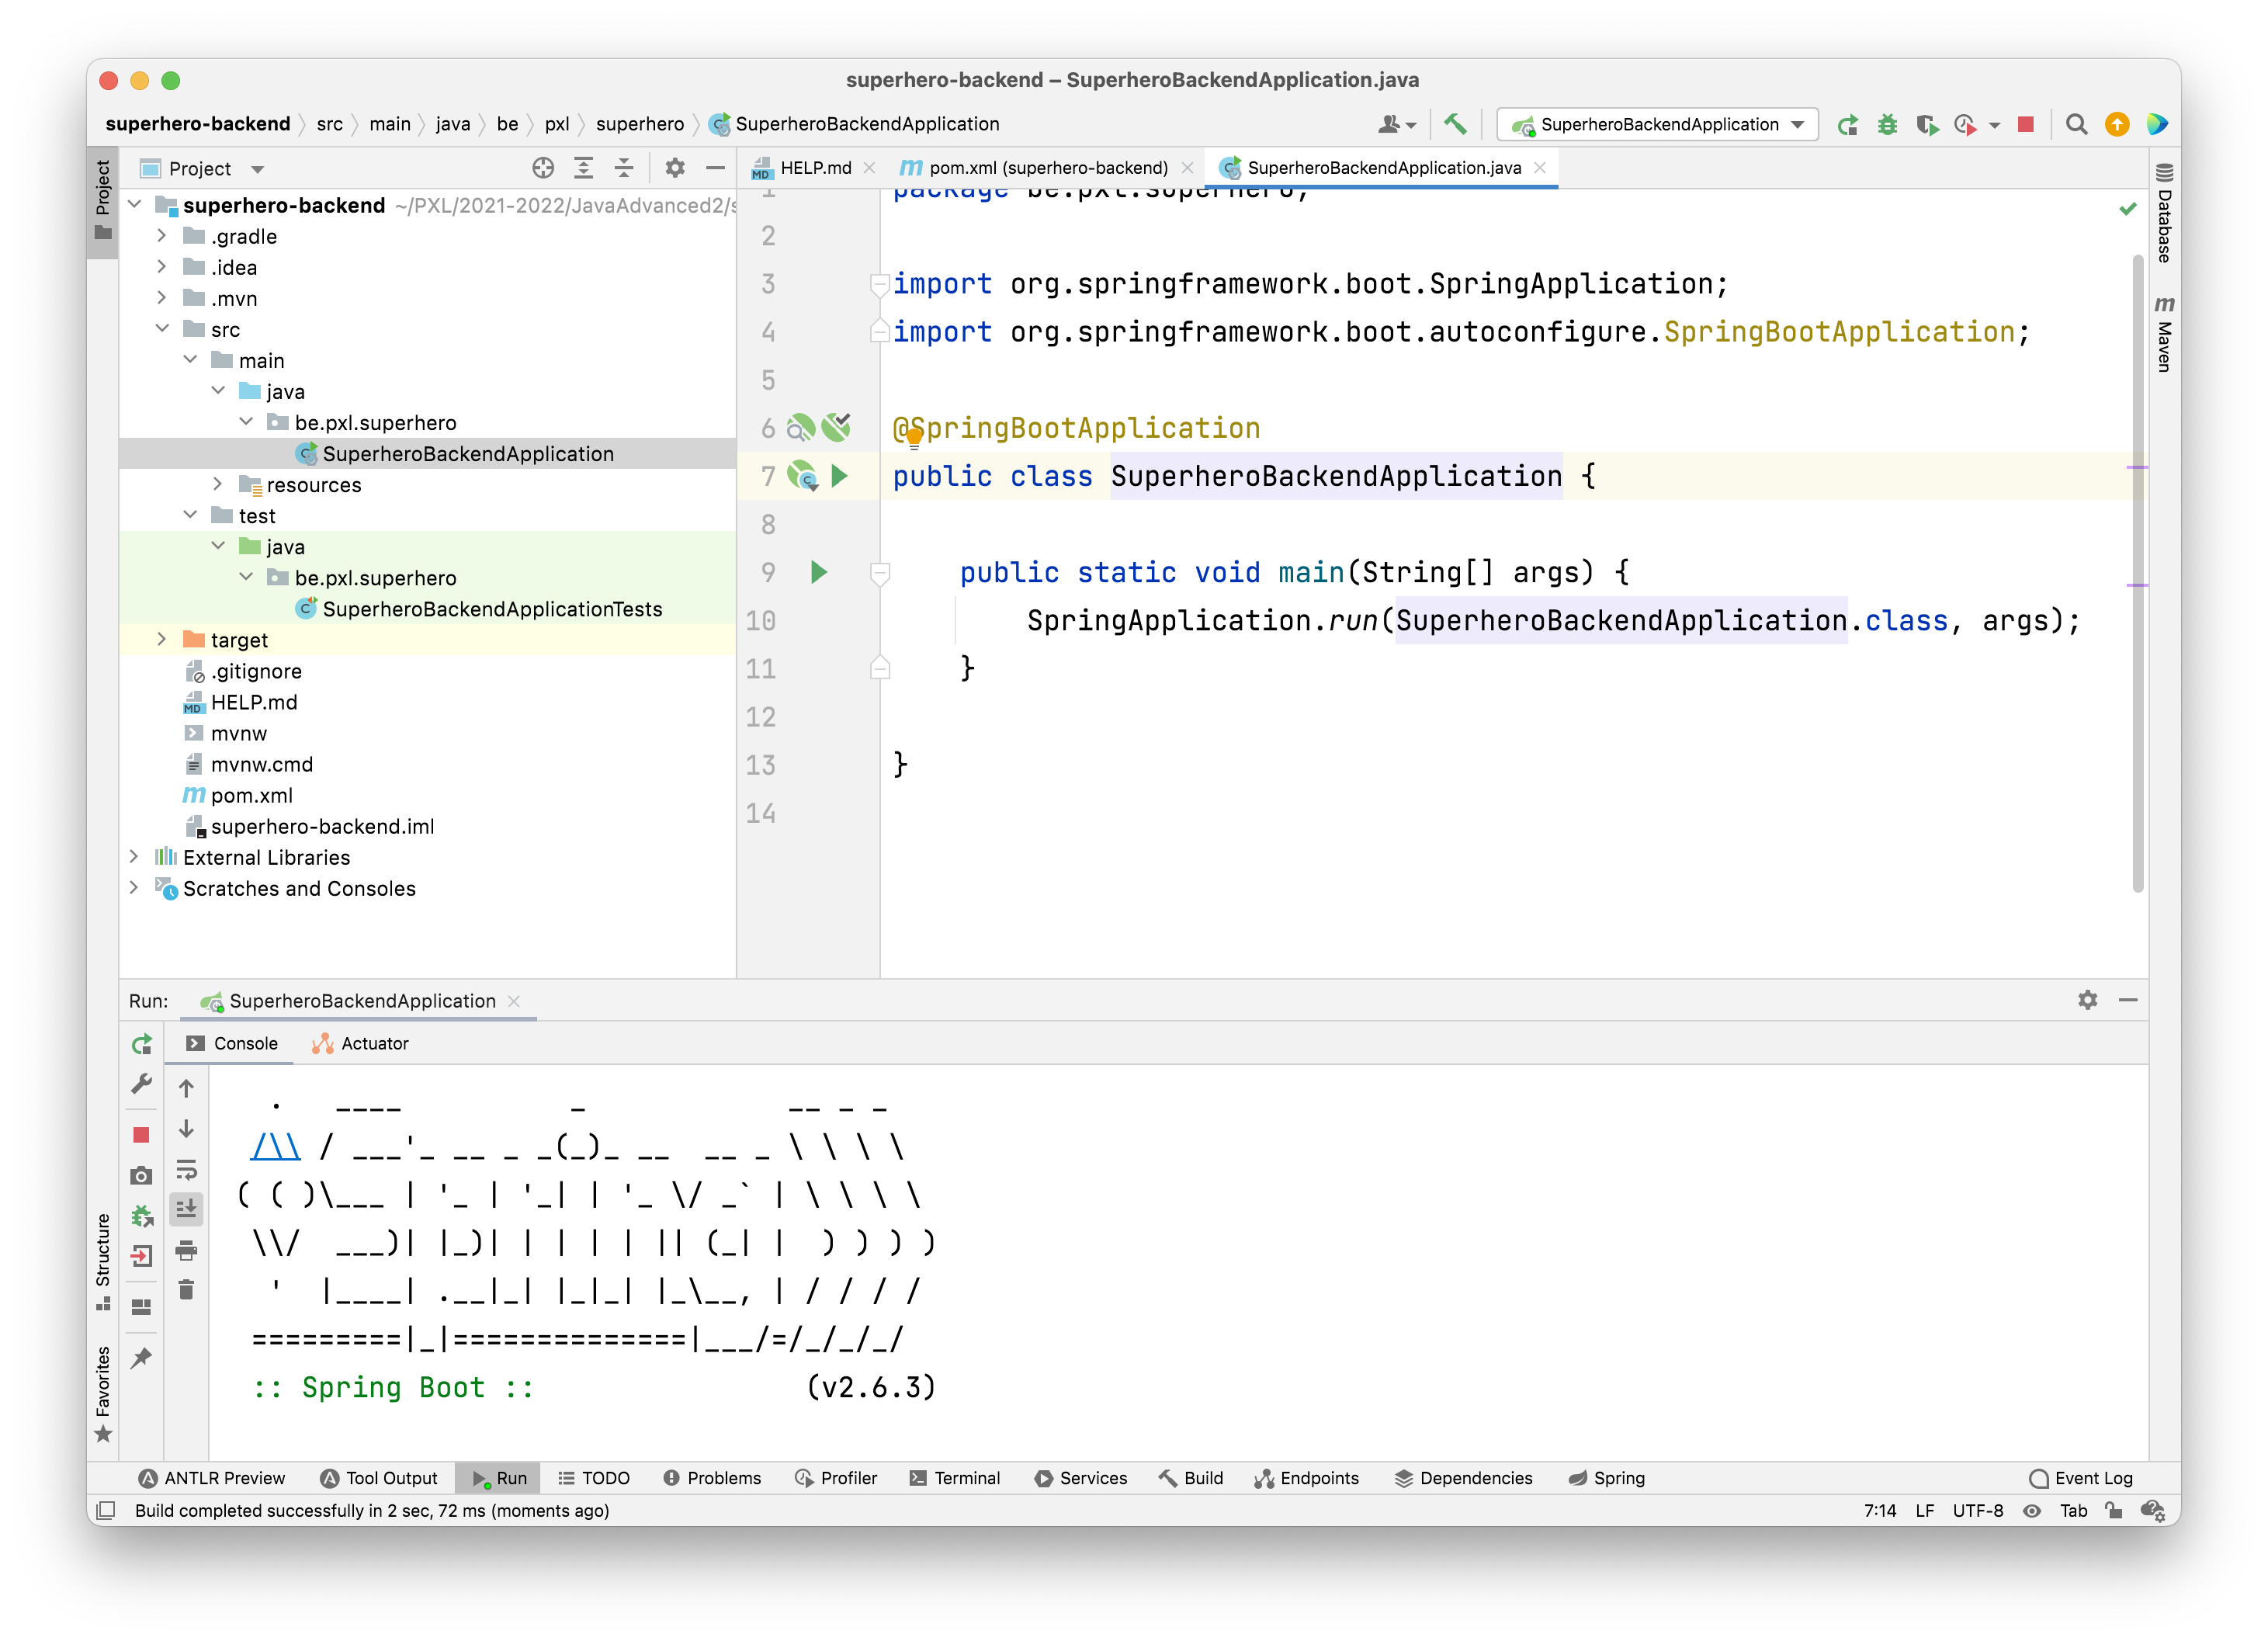
\includegraphics[width=\textwidth]{./images/chapter2/first-run.png}

Momenteel kan de Spring Boot applicatie enkel een whitelabel error pagina tonen.  De error pagina krijg je te zien als je een GET-request uitvoert voor URL \url{http://localhost:8080}.

\frame{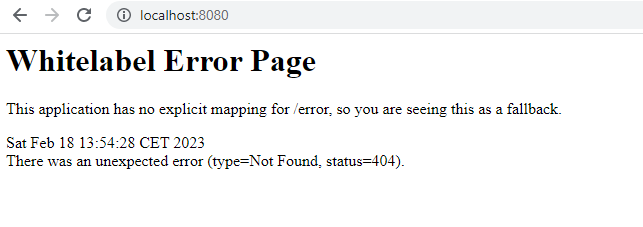
\includegraphics[width=\textwidth]{./images/chapter2/whitelabel_error_page.png}} 

Poort 8080 is de default poort van de Tomcat webserver.  Als deze poort al gebruikt wordt door een ander programma, krijg je de volgende foutmelding te zien.

\begin{lstlisting}[frame=single]
***************************
APPLICATION FAILED TO START
***************************

Description:

Web server failed to start. Port 8080 was already in use.
\end{lstlisting}

De poortnummer kan aangepast worden in het bestand application.properties.  Je gebruikt de eigenschap \textbf{server.port} om de gewenste poortnummer te kiezen.

\begin{lstlisting}[frame=single]
server.port=8081
\end{lstlisting}

\section{De RestController}

Spring boot heeft een annotatie voorzien voor de Spring bean die verantwoordelijk is voor het afhandelen van HTTP requests nl. @RestController. Spring boot heeft ook een annotatie @Controller, maar de @RestController zorgt ervoor dat het respons op het HTTP-request automatisch wordt omgezet (geserialiseerd) naar JSON of XML en wordt teruggestuurd naar de client.


\begin{lstlisting}[frame=single]
package be.pxl.demo.api;

import jakarta.annotation.PostConstruct;
import org.springframework.web.bind.annotation.GetMapping;
import org.springframework.web.bind.annotation.RestController;

import java.util.ArrayList;
import java.util.List;
import java.util.Random;

@RestController
@RequestMapping("/greetings")
public class GreetingController {

    private final List<String> messages = new ArrayList<>();
    private static final Random RANDOM = new Random();

    @PostConstruct
    public void init() {
        messages.add("Peek-a-boo!");
        messages.add("Howdy-doody!");
        messages.add("My name's Ralph, and I'm a bad guy.");
        messages.add("I come in peace!");
        messages.add("Put that cookie down!");

    }

    @GetMapping("/hello")
    public String doGreeting() {
        return messages.get(RANDOM.nextInt(messages.size()));
    }
}
\end{lstlisting}

De @RestController markeert de klasse GreetingController als een REST-controller.
De annotatie @RequestMapping("/greetings") specificeert het basispad voor alle requests die door deze controller worden afgehandeld.
@GetMapping("/hello") geeft aan dat de goGreeting-methode wordt uitgevoerd wanneer een HTTP GET-verzoek wordt gemaakt naar het pad "/greetings/hello". Het resultaat van deze methode wordt automatisch omgezet in tekst en teruggestuurd als de respons.

\begin{figure}[H]
  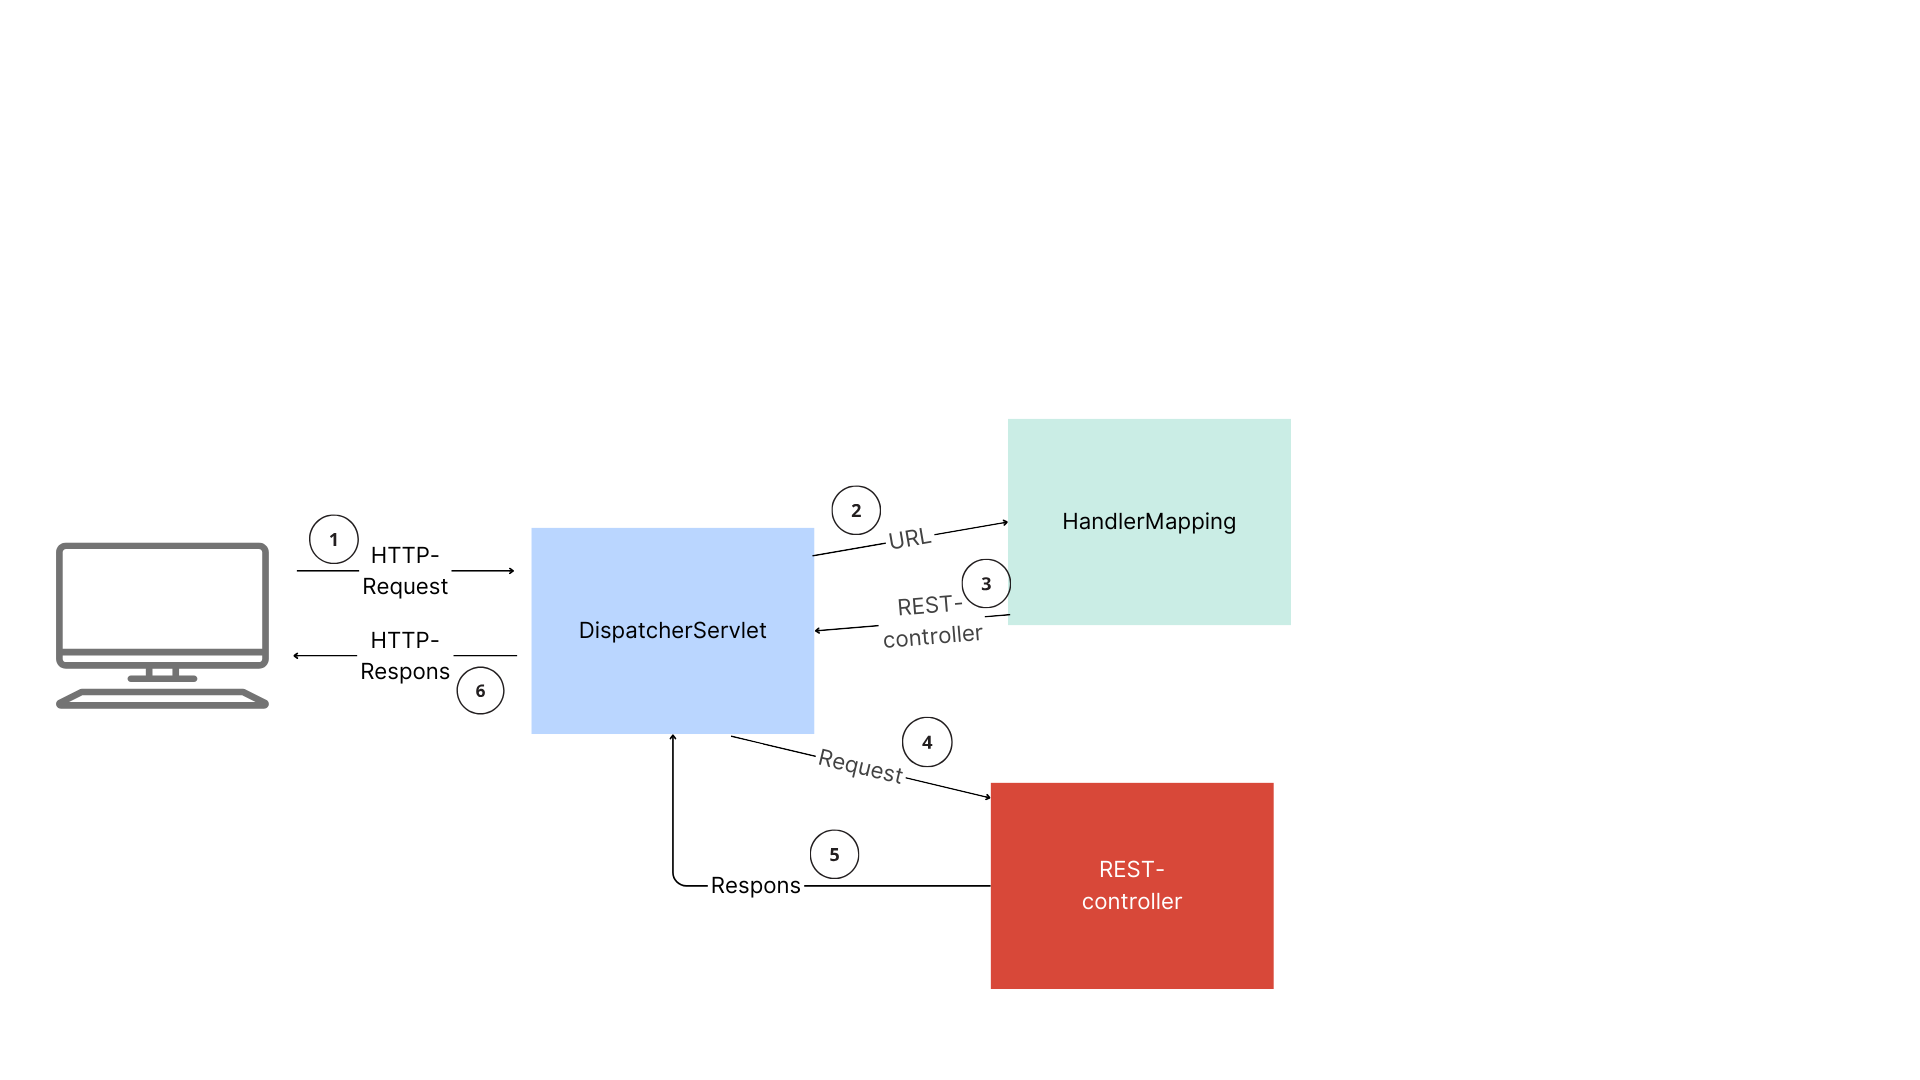
\includegraphics[width=\linewidth]{images/chapter-rest/dispatcherservlet.png}
  \caption{Een REST-verzoek afhandelen}
  \label{fig:test_passed}
\end{figure}

De component van Spring Boot die verantwoordelijk is dat een HTTP-request door de juiste REST-controller wordt afgehandeld is de DispatcherServlet.  De DispatcherServlet is onderdeel van Spring MVC.  De DispatcherServlet bepaalt welke controller een HTTP-request moet afhandelen,  hij geeft het request door aan de juiste controller en  verwerkt het respons van de controller om een HTTP-respons terug te sturen naar de client.

Om te achterhalen welke REST-controller verantwoordelijk is om een HTTP-request af te handelen raadpleegt de DispatcherServlet de HandlerMapping. De HandlerMapping is als het ware een kaart die URL's koppelt aan specifieke controllerklassen en methoden.
Op basis van de URL in het binnenkomende request bepaalt de DispatcherServlet welke controllerklasse en methode verantwoordelijk zijn voor het afhandelen van het request.


\begin{oefening}
Maak het package \textit{be.pxl.demo.api}.  Voeg de klasse \textbf{GreetingController} toe het package.  Start de Spring Boot applicatie en open de URL \url{http://localhost:8080/greetings/hello} in een browser. Voeg in de REST-controller een methode toe met de URI GET /greetings/daytime die de huidige dag en het tijdstip teruggeeft in het formaat 'Maandag 18 september 2023'.
\end{oefening}

\section{MusicPlaylist}

We gaan een nieuwe Spring Boot toepassing aanmaken waarmee we een muziek playlist beheren. 

\begin{oefening}
Maak een nieuwe Spring boot toepassing MusicPlaylist. We gebruiken Spring MVC om een RESTful web applicatie te maken.  
\end{oefening}

\subsection{Een liedje toevoegen aan een playlist}

\begin{apiRoute}{post}{/playlist/songs}{Add a new song to the playlist.}
\begin{routeRequest}{application/json}
\begin{routeRequestBody}
{
  "title": "Hello",
  "artist": "Adele",
  "duration_seconds": 293,
  "genre": "POP"
}
\end{routeRequestBody}
\end{routeRequest}
\begin{routeResponse}{application/json}
\begin{routeResponseItem}{200}{ok}
\end{routeResponseItem}
\end{routeResponse}
\end{apiRoute}


Om te beginnen hebben we de klasse Song nodig. 

\begin{lstlisting}[language=java,  frame=single]
public class Song {
    private String title;
    private String artist;
    @JsonProperty("duration_seconds")
    private int durationSeconds;
    private Genre genre;

    // Default constructor
    public Song() {
    }

    // Parameterized constructor
    public Song(String title, String artist, int durationSeconds, Genre genre) {
        this.title = title;
        this.artist = artist;
        this.durationSeconds = durationSeconds;
        this.genre = genre;
    }

    // Getter and setter methods
    public String getTitle() {
        return title;
    }

    public void setTitle(String title) {
        this.title = title;
    }

    public String getArtist() {
        return artist;
    }

    public void setArtist(String artist) {
        this.artist = artist;
    }

    public int getDurationSeconds() {
        return durationSeconds;
    }

    public void setDurationSeconds(int durationSeconds) {
        this.durationSeconds = durationSeconds;
    }

    public Genre getGenre() {
        return genre;
    }

    public void setGenre(Genre genre) {
        this.genre = genre;
    }

    @Override
    public String toString() {
        return "Song{" +
                "title='" + title + '\'' +
                ", artist='" + artist + '\'' +
                ", durationSeconds=" + durationSeconds +
                ", genre='" + genre + '\'' +
                '}';
    }
}
\end{lstlisting}


Nu gaan we de REST-controller implementeren.  We gaan hierin een methode voorzien die een POST op de URI /playlist/songs kan afhandelen.  Initieel gaan we enkel de titel in de loggegevens tonen. 

\begin{lstlisting}[language=java,  frame=single]
@RestController
@RequestMapping("/playlist/songs")
public class MusicPlaylistController {

	private static final Logger LOGGER = LoggerFactory.getLogger(MusicPlaylistController.class);

	@PostMapping
	public void addSong(@RequestBody Song song) {
		if (LOGGER.isInfoEnabled()) {
			LOGGER.info("Adding song [" + song.getTitle() + "]");
		}
	}
}
\end{lstlisting}

De liedjes die aan de playlist worden toegevoegd willen we bijhouden. Later zullen we ze wegschrijven in een databank, maar voorlopig gaan we ze bijhouden in een lijst.
Om dit mogelijk te maken gaan we een nieuwe Spring Bean toevoegen: de MusicPlaylistService.  

\begin{lstlisting}[language=java,  frame=single]
package be.pxl.demo;

import be.pxl.demo.domain.Song;
import org.springframework.stereotype.Service;

import java.util.ArrayList;
import java.util.List;

@Service
public class MusicPlaylistService {
	private final List<Song> myPlaylist = new ArrayList<>();

	public void addSong(Song song) {
		myPlaylist.add(song);
	}
}
\end{lstlisting}

De MusicPlaylistService wordt geannoteerd met @Service .
In onze Spring Boot applicaties gaan we steeds de business-logica implementeren in de service-laag.  De @Service annotatie wordt gebruikt voor de componenten (Spring Beans) in de service-laag.  Wanneer onze Spring Boot applicatie opstart wordt er exact \'e\'en instantie van de MusicPlaylistService aangemaakt in de ApplicationContext en deze instantie wordt tijdens de volledige levensduur van de toepassing gebruikt.  Dit noemen we de scope van de service en de default scope noemen we \textbf{singleton}. 
Dit betekent dat we \'e\'en enkele, gedeelde playlist hebben voor alle gebruikers.

Nu gaan we de MusicPlaylistService beschikbaar maken in de MusicPlaylistController.
We maken gebruik van \textbf{constructor injection}.  Zodra de instantie van de MusicPlaylistController door Spring Boot wordt aangemaakt, zal er eerst gezorgd worden dat de instantie MusicPlaylistService aangemaakt wordt. Deze instantie wordt dan achter de schermen meegegeven aan de constructor van de MusicPlaylistController. Zo kan ons MusicPlaylistController-object het MusicPlaylistService-object gebruiken.
Omdat er maar \'e\'en constructor is, is de annotatie @Autowired eigenlijk overbodig.

\begin{lstlisting}[language=java,  frame=single]
@RestController
@RequestMapping("/playlist/songs")
public class MusicPlaylistController {

	private static final Logger LOGGER = LoggerFactory.getLogger(MusicPlaylistController.class);
	private final MusicPlaylistService musicPlaylistService;

	@Autowired
	public MusicPlaylistController(MusicPlaylistService musicPlaylistService) {
		this.musicPlaylistService = musicPlaylistService;
	}

	@PostMapping
	public void addSong(@RequestBody Song song) {
		if (LOGGER.isInfoEnabled()) {
			LOGGER.info("Adding song [" + song.getTitle() + "]");
		}
		musicPlaylistService.addSong(song);
	}
}
\end{lstlisting}

Test nu het POST-verzoek.  Je kan Postman,  Insomnia of een andere tool gebruiken om een POST-verzoek naar de toepassing te sturen.  De toegevoegde liedjes gaan uiteraard verloren wanneer je de toepassing herstart. 

\begin{figure}[H]
  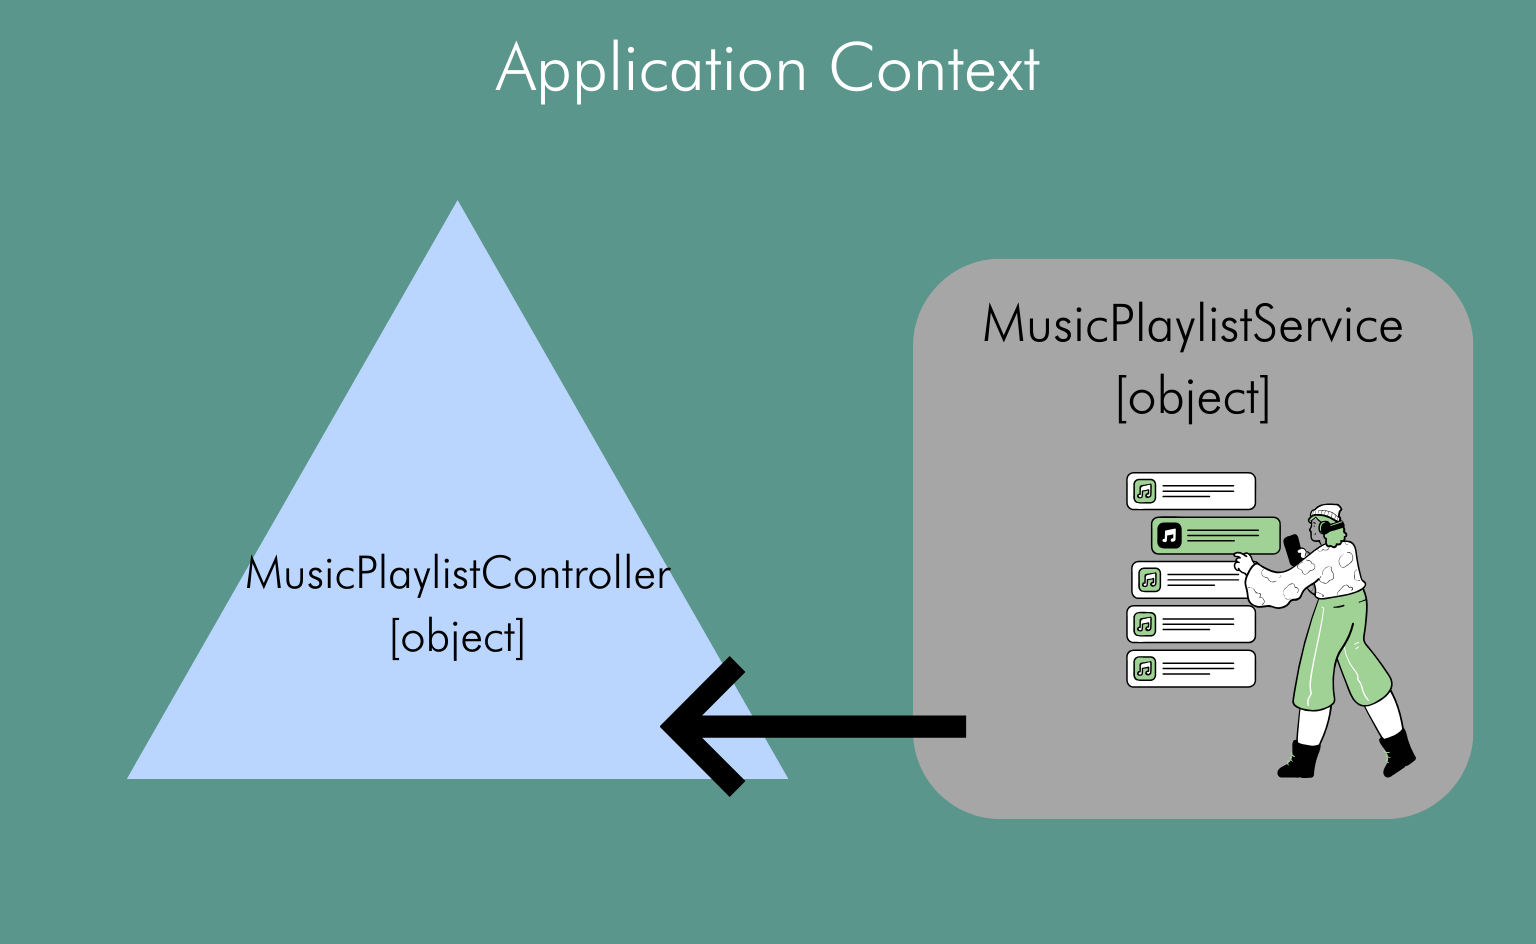
\includegraphics[width=\linewidth]{images/chapter-rest/applicationcontext_musicplaylist.png}
  \caption{Spring Beans in de Application Context}
  \label{fig:spring_beans_musicplaylist}
\end{figure}


\begin{figure}[H]
  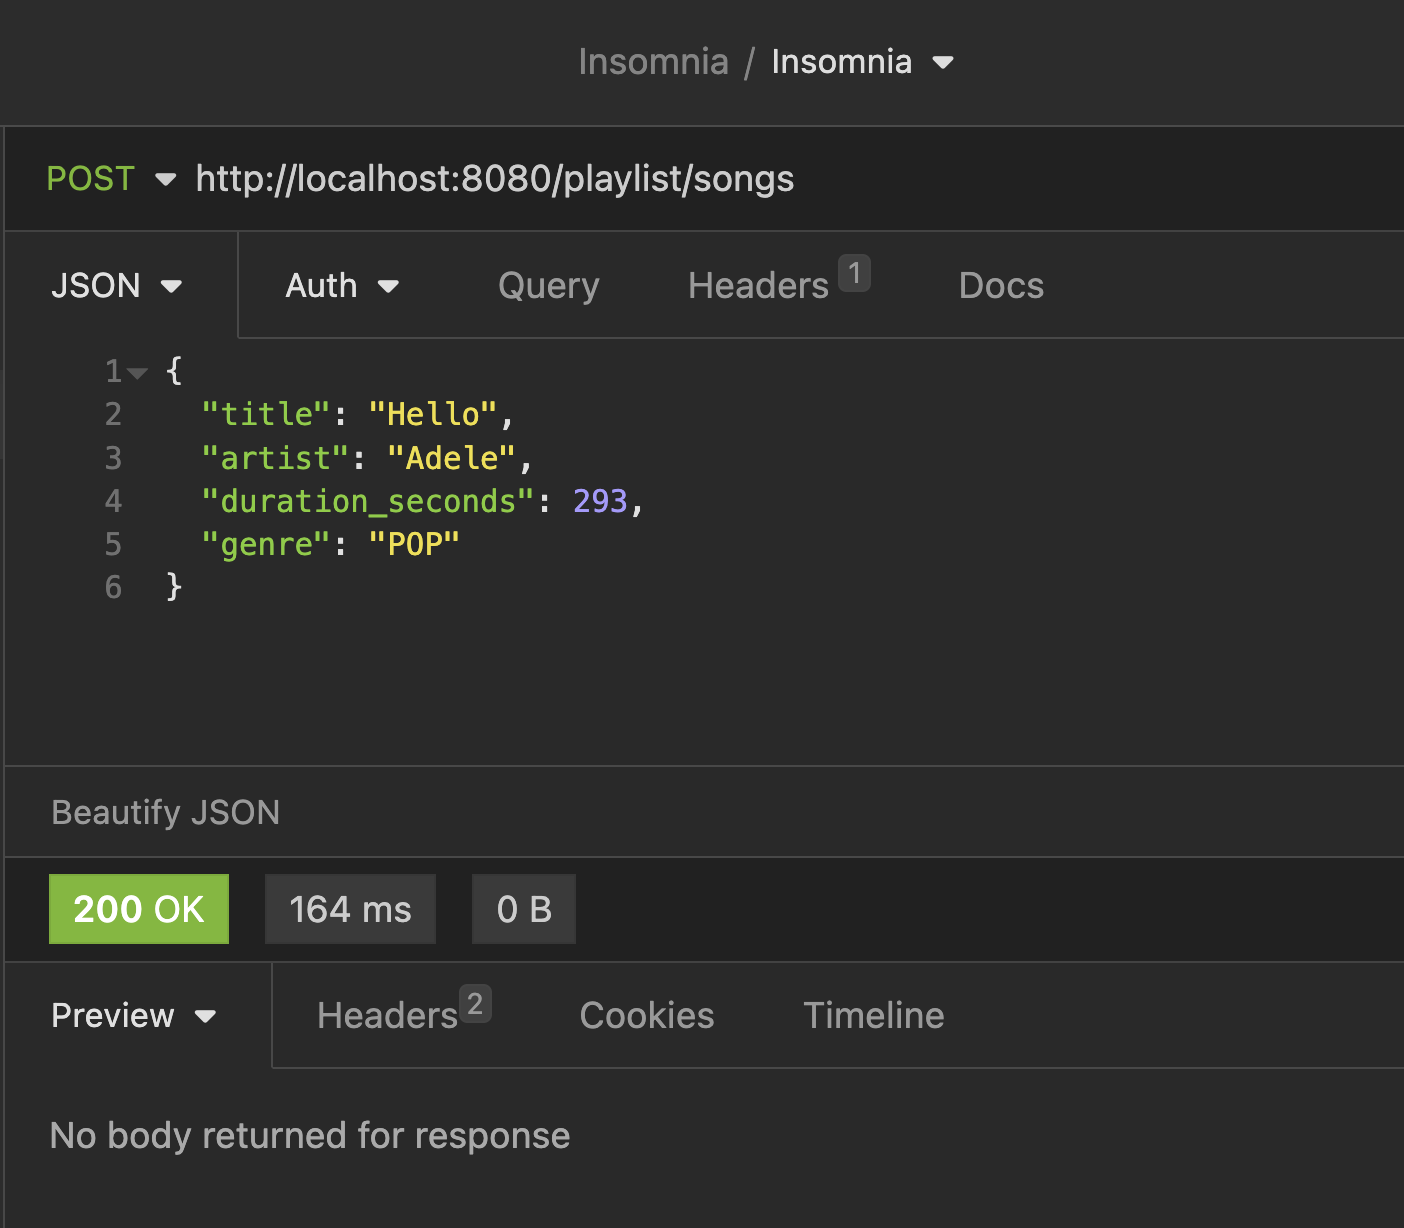
\includegraphics[width=\linewidth]{images/chapter-rest/insomnia_post.png}
  \caption{POST-verzoek met Insomnia}
  \label{fig:post_request}
\end{figure}

\subsection{De playlist opvragen}


\begin{apiRoute}{get}{/playlist/songs}{Retrieve all songs from the playlist}
\begin{routeParameter}
	\noRouteParameter {no parameter }
\end{routeParameter}
\begin{routeRequest}{application/json}
\end{routeRequest}
\begin{routeResponse}{application/json}
\begin{routeResponseItem}{200}{ok}
\begin{routeResponseItemBody}
[
	{
		"title": "Hello",
		"artist": "Adele",
		"genre": "POP",
		"duration_seconds": 293
	},
	{
		"title": "Shape of You",
		"artist": "Ed Sheeran",
		"genre": "POP",
		"duration_seconds": 233
	},
	{
		"title": "Umbrella",
		"artist": "Rihanna",
		"genre": "RNB",
		"duration_seconds": 264
	}
]
\end{routeResponseItemBody}
\end{routeResponseItem}
\end{routeResponse}
\end{apiRoute}


\begin{lstlisting}[language=java,  frame=single]
package be.pxl.demo;

import be.pxl.demo.domain.Song;
import org.springframework.stereotype.Service;

import java.util.ArrayList;
import java.util.List;

@Service
public class MusicPlaylistService {
	private final List<Song> myPlaylist = new ArrayList<>();

	public void addSong(Song song) {
		myPlaylist.add(song);
	}

	public List<Song> getSongs() {
		return myPlaylist;
	}
}
\end{lstlisting}


\begin{lstlisting}[language=java,  frame=single]
package be.pxl.demo.controller;

import be.pxl.demo.MusicPlaylistService;
import be.pxl.demo.domain.Song;
import org.slf4j.Logger;
import org.slf4j.LoggerFactory;
import org.springframework.beans.factory.annotation.Autowired;
import org.springframework.web.bind.annotation.GetMapping;
import org.springframework.web.bind.annotation.PostMapping;
import org.springframework.web.bind.annotation.RequestBody;
import org.springframework.web.bind.annotation.RequestMapping;
import org.springframework.web.bind.annotation.RestController;

import java.util.List;

@RestController
@RequestMapping("/playlist/songs")
public class MusicPlaylistController {

	private static final Logger LOGGER = LoggerFactory.getLogger(MusicPlaylistController.class);
	private final MusicPlaylistService musicPlaylistService;

	@Autowired
	public MusicPlaylistController(MusicPlaylistService musicPlaylistService) {
		this.musicPlaylistService = musicPlaylistService;
	}

	@PostMapping
	public void addSong(@RequestBody Song song) {
		if (LOGGER.isInfoEnabled()) {
			LOGGER.info("Adding song [" + song.getTitle() + "]");
		}
		musicPlaylistService.addSong(song);
	}

	@GetMapping
	public List<Song> getSongs() {
		return musicPlaylistService.getSongs();
	}
}
\end{lstlisting}

\subsection{Liedjes van \'e\'en genre}


 
 \begin{apiRoute}{get}{/playlist/songs/\{genre\}}{Retrieve all songs from the playlist with the given genre}
\begin{routeParameter}
	\routeParamItem{genre}{the requested genre}
\end{routeParameter}
\begin{routeRequest}{application/json}
\end{routeRequest}
\begin{routeResponse}{application/json}
\begin{routeResponseItem}{200}{ok}
\begin{routeResponseItemBody}
[
	{
		"title": "Hello",
		"artist": "Adele",
		"genre": "POP",
		"duration_seconds": 293
	},
	{
		"title": "Shape of You",
		"artist": "Ed Sheeran",
		"genre": "POP",
		"duration_seconds": 233
	}
]
\end{routeResponseItemBody}
\end{routeResponseItem}
\end{routeResponse}
\end{apiRoute}


\begin{lstlisting}[language=java,  frame=single]
package be.pxl.demo.controller;

import be.pxl.demo.MusicPlaylistService;
import be.pxl.demo.domain.Genre;
import be.pxl.demo.domain.Song;
import org.slf4j.Logger;
import org.slf4j.LoggerFactory;
import org.springframework.beans.factory.annotation.Autowired;
import org.springframework.web.bind.annotation.GetMapping;
import org.springframework.web.bind.annotation.PathVariable;
import org.springframework.web.bind.annotation.PostMapping;
import org.springframework.web.bind.annotation.RequestBody;
import org.springframework.web.bind.annotation.RequestMapping;
import org.springframework.web.bind.annotation.RestController;

import java.util.List;

@RestController
@RequestMapping("/playlist/songs")
public class MusicPlaylistController {

	private static final Logger LOGGER = LoggerFactory.getLogger(MusicPlaylistController.class);
	private final MusicPlaylistService musicPlaylistService;

	@Autowired
	public MusicPlaylistController(MusicPlaylistService musicPlaylistService) {
		this.musicPlaylistService = musicPlaylistService;
	}

	@PostMapping
	public void addSong(@RequestBody Song song) {
		if (LOGGER.isInfoEnabled()) {
			LOGGER.info("Adding song [" + song.getTitle() + "]");
		}
		musicPlaylistService.addSong(song);
	}

	@GetMapping
	public List<Song> getSongs() {
		return musicPlaylistService.getSongs();
	}

	@GetMapping("{genre}")
	public List<Song> getSongs(@PathVariable Genre genre) {
		return musicPlaylistService.getSongsByGenre(genre);
	}
}
\end{lstlisting}

\begin{lstlisting}[language=java,  frame=single]
package be.pxl.demo;

import be.pxl.demo.domain.Genre;
import be.pxl.demo.domain.Song;
import org.springframework.stereotype.Service;

import java.util.ArrayList;
import java.util.List;

@Service
public class MusicPlaylistService {
	private final List<Song> myPlaylist = new ArrayList<>();

	public void addSong(Song song) {
		myPlaylist.add(song);
	}

	public List<Song> getSongs() {
		return myPlaylist;
	}

	public List<Song> getSongsByGenre(Genre genre) {
		List<Song> response = new ArrayList<>();
		for (Song song : myPlaylist) {
			if (song.getGenre() == genre) {
				response.add(song);
			}
		}
		return response;
	}
}
\end{lstlisting}


\subsection{Gegevens van een liedje aanpassen}

Als je een nieuwe song in de playlist toevoegt, dan wordt deze steeds achteraan in de lijst toegevoegd. We kunnen nu de gegevens van het liedje op een gegeven positie in de lijst gaan overschrijven of aanpassen.  De index die we meegeven is een waarde van 0 tot 1 minder dan de lengte van de lijst.  Later zullen we zien hoe we een duidelijke foutboodschap kunnen geven aan de client als een foutieve index-waarde wordt gegeven.

Om de gegevens van een liedje aan te passen gebruiken we een PUT-verzoek. 
Je moet steeds alle gegevens van het liedje meegeven in de requestbody. 

\begin{apiRoute}{put}{/musicplaylist/songs\{index\}}{Update the song at the given index.}
\begin{routeParameter}
\routeParamItem{code}{unique identification of a house}
\end{routeParameter}
\begin{routeRequest}{application/json}
\begin{routeRequestBody}
{
		"title": "Hello",
		"artist": "Adele",
		"genre": "POP",
		"duration_seconds": 293
}
\end{routeRequestBody}
\end{routeRequest}
\begin{routeResponse}{application/json}
\begin{routeResponseItem}{200}{ok}
\end{routeResponseItem}
\end{routeResponse}
\end{apiRoute}


\begin{lstlisting}
package be.pxl.demo.controller;

import be.pxl.demo.MusicPlaylistService;
import be.pxl.demo.domain.Genre;
import be.pxl.demo.domain.Song;
import org.slf4j.Logger;
import org.slf4j.LoggerFactory;
import org.springframework.beans.factory.annotation.Autowired;
import org.springframework.web.bind.annotation.DeleteMapping;
import org.springframework.web.bind.annotation.GetMapping;
import org.springframework.web.bind.annotation.PathVariable;
import org.springframework.web.bind.annotation.PostMapping;
import org.springframework.web.bind.annotation.PutMapping;
import org.springframework.web.bind.annotation.RequestBody;
import org.springframework.web.bind.annotation.RequestMapping;
import org.springframework.web.bind.annotation.RestController;

import java.util.List;

@RestController
@RequestMapping("/playlist/songs")
public class MusicPlaylistController {

	private static final Logger LOGGER = LoggerFactory.getLogger(MusicPlaylistController.class);
	private final MusicPlaylistService musicPlaylistService;

	@Autowired
	public MusicPlaylistController(MusicPlaylistService musicPlaylistService) {
		this.musicPlaylistService = musicPlaylistService;
	}

	@PostMapping
	public void addSong(@RequestBody Song song) {
		if (LOGGER.isInfoEnabled()) {
			LOGGER.info("Adding song [" + song.getTitle() + "]");
		}
		musicPlaylistService.addSong(song);
	}

	@GetMapping
	public List<Song> getSongs() {
		return musicPlaylistService.getSongs();
	}

	@GetMapping("/{genre}")
	public List<Song> getSongs(@PathVariable Genre genre) {
		return musicPlaylistService.getSongsByGenre(genre);
	}

	@PutMapping("/{index}")
	public void updateSong(@PathVariable int index, @RequestBody Song song) {
		musicPlaylistService.updateSong(index, song);
	}
}
\end{lstlisting}

\begin{lstlisting}
package be.pxl.demo;

import be.pxl.demo.domain.Genre;
import be.pxl.demo.domain.Song;
import org.springframework.stereotype.Service;

import java.util.ArrayList;
import java.util.List;

@Service
public class MusicPlaylistService {
	private final List<Song> myPlaylist = new ArrayList<>();

	public void addSong(Song song) {
		myPlaylist.add(song);
	}

	public List<Song> getSongs() {
		return myPlaylist;
	}

	public List<Song> getSongsByGenre(Genre genre) {
		List<Song> response = new ArrayList<>();
		for (Song song : myPlaylist) {
			if (song.getGenre() == genre) {
				response.add(song);
			}
		}
		return response;
	}

	public void updateSong(int index, Song song) {
		myPlaylist.set(index, song);
	}

	public void deleteSong(int index) {
		myPlaylist.remove(index);
	}
}
\end{lstlisting}

We vervangen het liedje op de opgegeven index door een nieuw Song-object met de aangepaste gegevens.

\subsection{Een liedje verwijderen}

Om een liedje op een opgegeven index uit de playlist te verwijderen gaan we een DELETE-verzoek implementeren.


\begin{apiRoute}{delete}{/musicplaylist/songs/\{index\}}{Delete the song at the given index.}
\begin{routeParameter}
\routeParamItem{index}{position of the song to be deleted}
\end{routeParameter}
\begin{routeResponse}{application/json}
\begin{routeResponseItem}{200}{ok}
\end{routeResponseItem}
\end{routeResponse}
\end{apiRoute}

\begin{lstlisting}
package be.pxl.demo.controller;

import be.pxl.demo.MusicPlaylistService;
import be.pxl.demo.domain.Genre;
import be.pxl.demo.domain.Song;
import org.slf4j.Logger;
import org.slf4j.LoggerFactory;
import org.springframework.beans.factory.annotation.Autowired;
import org.springframework.web.bind.annotation.DeleteMapping;
import org.springframework.web.bind.annotation.GetMapping;
import org.springframework.web.bind.annotation.PathVariable;
import org.springframework.web.bind.annotation.PostMapping;
import org.springframework.web.bind.annotation.PutMapping;
import org.springframework.web.bind.annotation.RequestBody;
import org.springframework.web.bind.annotation.RequestMapping;
import org.springframework.web.bind.annotation.RestController;

import java.util.List;

@RestController
@RequestMapping("/playlist/songs")
public class MusicPlaylistController {

	private static final Logger LOGGER = LoggerFactory.getLogger(MusicPlaylistController.class);
	private final MusicPlaylistService musicPlaylistService;

	@Autowired
	public MusicPlaylistController(MusicPlaylistService musicPlaylistService) {
		this.musicPlaylistService = musicPlaylistService;
	}

	@PostMapping
	public void addSong(@RequestBody Song song) {
		if (LOGGER.isInfoEnabled()) {
			LOGGER.info("Adding song [" + song.getTitle() + "]");
		}
		musicPlaylistService.addSong(song);
	}

	@GetMapping
	public List<Song> getSongs() {
		return musicPlaylistService.getSongs();
	}

	@GetMapping("/{genre}")
	public List<Song> getSongs(@PathVariable Genre genre) {
		return musicPlaylistService.getSongsByGenre(genre);
	}

	@PutMapping("/{index}")
	public void updateSong(@PathVariable int index, @RequestBody Song song) {
		musicPlaylistService.updateSong(index, song);
	}

	@DeleteMapping("/{index}")
	public void updateSong(@PathVariable int index) {
		musicPlaylistService.deleteSong(index);
	}
}
\end{lstlisting}


\begin{lstlisting}
package be.pxl.demo;

import be.pxl.demo.domain.Genre;
import be.pxl.demo.domain.Song;
import org.springframework.stereotype.Service;

import java.util.ArrayList;
import java.util.List;

@Service
public class MusicPlaylistService {
	private final List<Song> myPlaylist = new ArrayList<>();

	public void addSong(Song song) {
		myPlaylist.add(song);
	}

	public List<Song> getSongs() {
		return myPlaylist;
	}

	public List<Song> getSongsByGenre(Genre genre) {
		List<Song> response = new ArrayList<>();
		for (Song song : myPlaylist) {
			if (song.getGenre() == genre) {
				response.add(song);
			}
		}
		return response;
	}

	public void updateSong(int index, Song song) {
		myPlaylist.set(index, song);
	}

	public void deleteSong(int index) {
		myPlaylist.remove(index);
	}
}
\end{lstlisting}


\begin{oefening}\textbf{Huizenjacht}
We maken een Spring Boot toepassing om het aanbod op de huizenmarkt te beheren.
Ontwikkel een RESTful web toepassing met onderstaande endpoints.
Je voorziet een component HouseService met \'e\'en enkele, gedeelde lijst van woningen  voor alle gebruikers.

Een huis wordt voorgesteld als een resource met volgende eigenschappen:

\begin{itemize}
  \item \texttt{code} (string): Unieke identificatie van het huis.
  \item \texttt{name} (string): Naam of beschrijving van het huis.
  \item \texttt{status} (enum): Status FOR\_SALE of SOLD.
  \item \texttt{city} (string): Locatie van het huis.
  \item \texttt{price} (double): Prijs van het huis.
\end{itemize}

\section{REST Endpoints}

\begin{apiRoute}{post}{/houses}{Create a new house.}
\begin{routeParameter}
	\noRouteParameter {no parameter }
\end{routeParameter}
\begin{routeRequest}{application/json}
\begin{routeRequestBody}
{
  "code": "HAS_001",
  "name": "Beautiful house in the city",
  "city": "Hasselt",
  "price": 250000
}
\end{routeRequestBody}
\end{routeRequest}
\begin{routeResponse}{application/json}
\begin{routeResponseItem}{200}{ok}
\end{routeResponseItem}
\end{routeResponse}
\end{apiRoute}


\begin{apiRoute}{put}{/houses/\{code\}}{Update the data (status, price,...) of the house with the given code.}
\begin{routeParameter}
\routeParamItem{code}{unique identification of a house}
\end{routeParameter}
\begin{routeRequest}{application/json}
\begin{routeRequestBody}
{
  "status": "SOLD"
  "name": "Beautiful house in the city",
  "price": 320000
}
\end{routeRequestBody}
\end{routeRequest}
\begin{routeResponse}{application/json}
\begin{routeResponseItem}{200}{ok}
\end{routeResponseItem}
\end{routeResponse}
\end{apiRoute}

\begin{apiRoute}{get}{/houses}{Retrieve all houses.}
\begin{routeParameter}
	\noRouteParameter {no parameter }
\end{routeParameter}
\begin{routeResponse}{application/json}
\begin{routeResponseItem}{200}{ok}
\begin{routeResponseItemBody}
[
  {
    "code": "GNK_001",
    "name": "Beautiful house in the city",
    "status": "SOLD",
     "city": "Genk",
    "price": 250000
  },
  {
    "code": "HAS_003",
    "name": "Cozy bungalow",
    "status": "FOR_SALE",
     "city": "Hasselt",
    "price": 180000
  }
]
\end{routeResponseItemBody}
\end{routeResponseItem}
\end{routeResponse}
\end{apiRoute}

\begin{apiRoute}{delete}{/houses/\{code\}}{Delete the house with the given code.}
\begin{routeParameter}
\routeParamItem{code}{unique identification of a house}
\end{routeParameter}
\begin{routeResponse}{application/json}
\begin{routeResponseItem}{200}{ok}
\end{routeResponseItem}
\end{routeResponse}
\end{apiRoute}

\end{oefening}

\chapter{Servlets}

\fcolorbox{black}[HTML]{E9F0E9}{\parbox{\textwidth}{%
\noindent \textbf{Learning goals}\\
The junior-colleague
\begin{enumerate}[nolistsep]
\item can explain what a Servlet is
\item can explain how Spring Boot uses Servlet technology (DispatcherServlet!)
\item can explain and use the lifecycle moments of a Servlet
\item can explain the usage of @WebServlet, @WebFilter and @WebListener
\item can explain the usage of HttpSession
\item can create an HTTPServlet to handle requests
\item can use cookies and HTTPSession in a web application
\item can use WebClient to send a simple HTTP request 
\item can implement a @WebFilter
\item can implement a @WebListener
\item can explain the Model-View-Controller design pattern
\item can explain the role of DispatcherServlet in Spring
\item can consume Rest services with WebClient
\item can implement a simple view with Thymeleaf
\end{enumerate}
}}

\fcolorbox{black}[HTML]{ADD8E6}{\parbox{\textwidth}{%
\noindent \textbf{Source for this chapter:}\\
\url{https://github.com/custersnele/servlet_technology.git}
}}

\section{What is a Servlet}

Relatively few applications still use Servlets directly,  but they're still the underlying technology behind the vast majority of Java and JVM web frameworks.
A servlet’s job is to take a client’s request and send back a response.
For example, we can use a Servlet to collect input from a user through an HTML form, query records from a database, and create web pages dynamically.
Servlets are under the control of another Java application called a Servlet Container. When an application running in a web server receives a request, the server hands the request to the Servlet Container – which in turn passes it to the target Servlet.
Java servlets typically run on the HTTP protocol. 

When using Spring Boot, the @ServletComponentScan annotation automatically registers the Servlet components for embedded web servers. This annotation supports the following Servlet 3.0 annotations:
\begin{itemize}
\item @WebServlet annotation
\item @WebFilter annotation
\item @WebListener annotation
\end{itemize}

\begin{lstlisting}
package be.pxl.paj.servlets;

import org.springframework.boot.SpringApplication;
import org.springframework.boot.autoconfigure.SpringBootApplication;
import org.springframework.boot.web.servlet.ServletComponentScan;

@SpringBootApplication
@ServletComponentScan
public class ServletDemoApplication {

	public static void main(String[] args) {
		SpringApplication.run(ServletDemoApplication.class, args);
	}
}
\end{lstlisting}

\section{Servlet class hierarchy}

The Servlet interface is the root interface of the servlet class hierarchy. All Servlets need to either directly or indirectly implement the Servlet interface. 

The Servlet interface of the jakarta.servlet package defines the methods that the Servlet container calls to manage the servlet life cycle. 

The GenericServlet class of the Servlet API implements the Servlet interface.

To develop a servlet that communicates using HTTP, we need to extend the HttpServlet class.

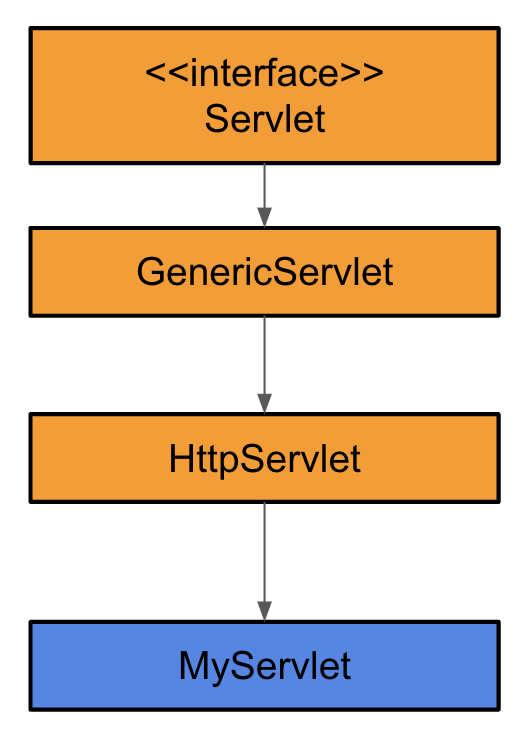
\includegraphics{./images/chapter8/servlet_hierarchy}


\section{Lifecycle of a servlet}

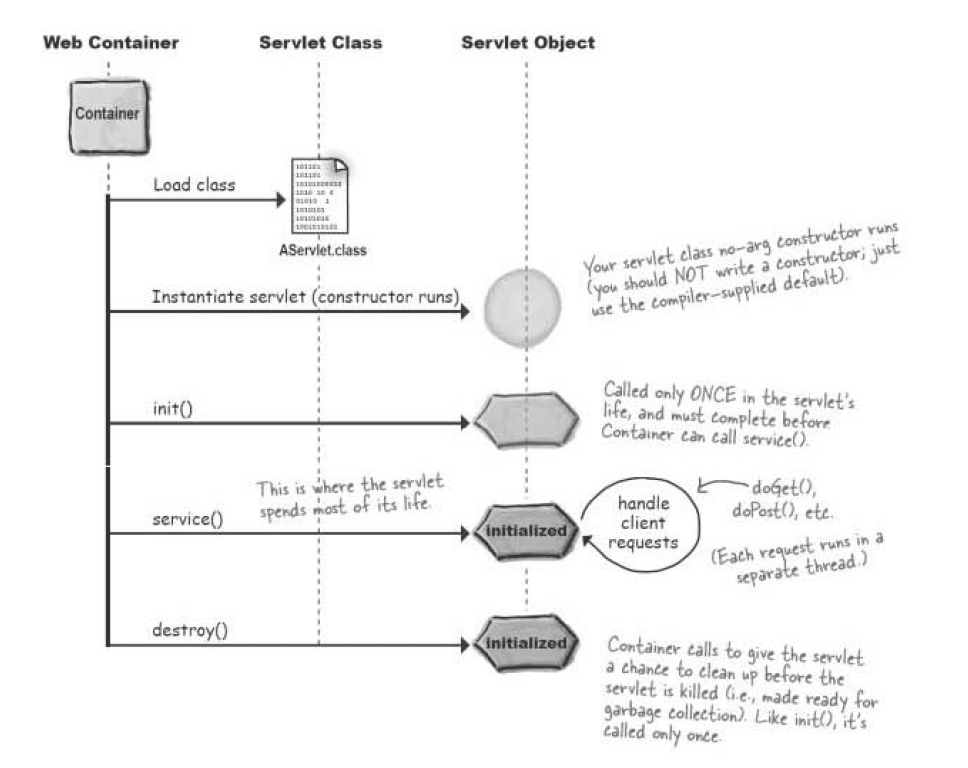
\includegraphics[width=\textwidth]{./images/chapter8/servlet_lifecycle}

The Servlet life cycle mainly goes through three stages:\cite{servlet_lifecycle}

\begin{itemize}
\item \textbf{Loading and initializing a Servlet.} After the Servlet is instantiated successfully, the Servlet container initializes the instantiated Servlet object. The container initializes the Servlet object by invoking the \textbf{init()} method. The jakarta.servlet.ServletConfig interface is implemented by a Servlet container to pass configuration information to a servlet, during initialization of a servlet.
\item \textbf{Request handling.} After initialization, the Servlet instance is ready to serve the client requests.  The Servlet's \textbf{service()} method is invoked to handle a client request. When multiple client requests come, the server will create multiple threads. Each client request corresponds to a thread that calls the Servlet's service() method.  That's the nice thing about Java, it's multithreaded and different threads (HTTP requests) can make use of the same instance. It would otherwise be too expensive to recreate, init() and destroy() them for every single request. If you encounter threadsafety issues when using servlets, then it is your fault, not Java's nor Servlet's fault.
\item \textbf{Destroying the Servlet.} When a Servlet container decides to destroy the Servlet,  all currently running threads can complete their jobs and next, the Servlet container calls the destroy() method on the Servlet instance.
\end{itemize}

\subsection{Example 1}

\begin{lstlisting}[language=java, frame=single]
package be.pxl.paj.servlets;

import jakarta.servlet.annotation.WebServlet;
import jakarta.servlet.http.HttpServlet;
import jakarta.servlet.http.HttpServletRequest;
import jakarta.servlet.http.HttpServletResponse;
import java.io.IOException;
import java.io.PrintWriter;
import java.time.LocalDateTime;
import java.time.format.DateTimeFormatter;
import java.util.Locale;

@WebServlet(value="/DateTimeServlet")
public class DateTimeServlet extends HttpServlet {

	private static final DateTimeFormatter FORMATTER_EN = DateTimeFormatter.ofPattern("EEEE dd/MM/yyyy HH:mm:ss", Locale.ENGLISH);
	private static final DateTimeFormatter FORMATTER_NL = DateTimeFormatter.ofPattern("EEEE dd/MM/yyyy HH:mm:ss", new Locale("nl"));

	@Override
	protected void doGet(HttpServletRequest req, HttpServletResponse resp) throws IOException {
		PrintWriter writer = resp.getWriter();
		String language = req.getParameter("lang");
		LocalDateTime dateTime = LocalDateTime.now();
		String dateAsText = "nl".equals(language) ? 
		         FORMATTER_NL.format(dateTime) : FORMATTER_EN.format(dateTime);
		writer.println("<html>" +
				"<body>" +
				"<h1 style=\"text-align:center\">" + dateAsText + "</h1></body>" +
				"</html>");
	}
}
\end{lstlisting}


\subsection{Example 2}


\begin{lstlisting}[frame=single, language=html]
<!DOCTYPE html>
<html lang="en">
<head>
	<meta charset="UTF-8">
	<title>Beer selection</title>
</head>
<body>
<h1>Beer Selection</h1>
<form method="POST" action="/SelectBeer.do">
	<p>Select beer characteristics:</p>
	<label for="color">Color:</label>
	<select id="color" name="color" size="1">
		<option value="light">Light</option>
		<option value="amber">Amber</option>
		<option value="brown">Brown</option>
		<option value="dark">Dark</option>
	</select>
	<br/>
	<br/>
	<input type="submit" />
</form>
</body>
</html>
\end{lstlisting}

\begin{lstlisting}[frame=single, language=java]
package be.pxl.paj.servlets;

import be.pxl.paj.servlets.service.BeerExpert;
import org.springframework.beans.factory.annotation.Autowired;

import jakarta.servlet.ServletException;
import jakarta.servlet.annotation.WebServlet;
import jakarta.servlet.http.HttpServlet;
import jakarta.servlet.http.HttpServletRequest;
import jakarta.servlet.http.HttpServletResponse;
import java.io.IOException;
import java.io.PrintWriter;
import java.util.List;

@WebServlet(value = "/SelectBeer.do")
public class SelectBeerServlet extends HttpServlet {

	private final BeerExpert beerExpert;

	@Autowired
	public SelectBeerServlet(BeerExpert beerExpert) {
		this.beerExpert = beerExpert;
	}

	@Override
	protected void doPost(HttpServletRequest req, HttpServletResponse resp) throws ServletException, IOException {
		String color = req.getParameter("color");

		List<String> result = beerExpert.getBrands(color);
		PrintWriter writer = resp.getWriter();

		writer.println("<html>" +
				"<body>" +
				"<h1 style=\"text-align:center\">Try these beers:</h1><p>" +
				String.join(", ", result) +
				"</p></body>" +
				"</html>");
	}
}
\end{lstlisting}

\begin{lstlisting}[frame=single, language=java]
package be.pxl.paj.servlets.service;

import org.springframework.stereotype.Service;

import java.util.ArrayList;
import java.util.List;

@Service
public class BeerExpert {

	public List<String> getBrands(String color) {
		List<String> brands = new ArrayList<>();
		if (color.equals("amber")) {
			brands.add("Jack Amber");
			brands.add("Red Moose");
		} else {
			brands.add("Jail Pale Ale");
			brands.add("Gout Stout");
		}
		return brands;
	}
}
\end{lstlisting}


\section{Session tracking}

Session management is a way to maintain state of an user. 

HTTP protocol is a stateless so we need to maintain state using session management techniques. Each time user requests to the server, server treats the request as the new request. 

There are several techniques for session management:

\begin{itemize}
\item Cookies
\item Hidden Form Field
\item URL Rewriting
\item HttpSession
\end{itemize}

In this course we will provide examples for using cookies and HttpSession.

\subsection{Cookies}

The method getCookies() in HttpServletRequest returns an array containing all of the Cookie objects the client sent with this request. 

\begin{lstlisting}[language=java, frame=single]
package be.pxl.paj.servlets;

import jakarta.servlet.annotation.WebServlet;
import jakarta.servlet.http.Cookie;
import jakarta.servlet.http.HttpServlet;
import jakarta.servlet.http.HttpServletRequest;
import jakarta.servlet.http.HttpServletResponse;
import java.io.IOException;
import java.io.PrintWriter;

@WebServlet(name = "Cookies", value = "/Cookies")
public class UsingCookies extends HttpServlet {

	public void doGet(HttpServletRequest request, HttpServletResponse response)
			throws IOException {
		response.setContentType("text/html");
		PrintWriter out = response.getWriter();

		out.println("<HTML>");
		out.println("<HEAD>");
		out.println("<TITLE>");
		out.println("A Web Page");
		out.println("</TITLE>");
		out.println("</HEAD>");
		out.println("<BODY");

		Cookie[] cookies = request.getCookies();
		boolean foundCookie = false;

		for (int loopIndex = 0; loopIndex < cookies.length; loopIndex++) {
			Cookie cookie1 = cookies[loopIndex];
			if (cookie1.getName().equals("color")) {
				out.println("bgcolor = " + cookie1.getValue());
				foundCookie = true;
			}
		}

		if (!foundCookie) {
			Cookie cookie1 = new Cookie("color", "cyan");
			cookie1.setMaxAge(24 * 60 * 60);
			response.addCookie(cookie1);
		}

		out.println(">");
		out.println("<H1>Setting and Reading Cookies</H1>");
		out.println("This page will set its background color using a cookie when reloaded.");
		out.println("</BODY>");
		out.println("</HTML>");
	}
}
\end{lstlisting}

\subsection{HttpSession}

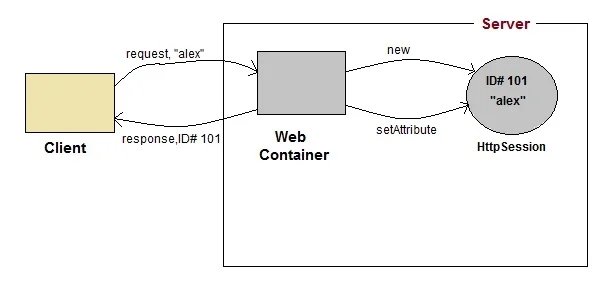
\includegraphics[width=\textwidth]{./images/chapter8/httpsession}

HTTP sessions are identified by a unique session ID.  A session ID is a pseudo-random number generated at the runtime. 

On client's first request, the Web Container generates a unique session ID and gives it back to the client encapsulated in the response. 
The client sends back the session ID with each request. This way the web container can identify where the request is coming from.
The Web Container uses this ID, finds the matching session with the ID and associates the session with the request.

Session hijacking is a known attack for HTTP sessions and can be prevented if all the requests going over the network are enforced to be over a secure connection (meaning, HTTPS).

Below is the click\_the\_button.html file.  There are several directories where you can store static html pages. In our demo we've chosen to create a folder named `static' in the application's resources folder.
\begin{lstlisting}[language=html]
<!DOCTYPE html>
<html lang="en">
<head>
	<meta charset="UTF-8">
	<title>Click the Button!</title>
</head>
<body>
<h1>Click the button!</h1>
<form action="/ButtonClicked" method="POST">
	<input type="submit" value="Click me!">
</form>
</body>
</html>
\end{lstlisting}

\begin{lstlisting}[language=java, frame=single]
package be.pxl.paj.servlets;

import java.io.IOException;

import jakarta.servlet.ServletException;
import jakarta.servlet.annotation.WebServlet;
import jakarta.servlet.http.HttpServlet;
import jakarta.servlet.http.HttpServletRequest;
import jakarta.servlet.http.HttpServletResponse;
import jakarta.servlet.http.HttpSession;

@WebServlet(name = "/ButtonClicked", value="/ButtonClicked")
public class ButtonClickedServlet extends HttpServlet {

	@Override
	public void doPost(HttpServletRequest request, 
	                                 HttpServletResponse response) throws IOException, ServletException {

		int clickCount = 0;

		//get the session, which contains user-specific data
		HttpSession session = request.getSession();

		if(session.getAttribute("clickCount") != null){
			//we've already stored the clickCount in a previous request, so get it
			clickCount = (int) session.getAttribute("clickCount");
		}

		clickCount++;

		//store the new clickCount in the session
		session.setAttribute("clickCount", clickCount);

		//output the clickCount for this user
		response.getOutputStream().println("<h1>You clicked the button " + clickCount + " times.</h1>");
		response.getOutputStream().println("<p>Click <a href=\"/click_the_button.html\">here</a> to go back to the button.</p>");
	}
}
\end{lstlisting}


\section{Spring DispatcherServlet}


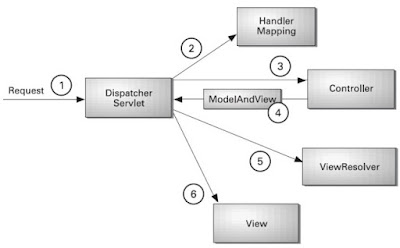
\includegraphics{./images/chapter8/spring_mvc}

The Spring web framework is built around the MVC (Model-View-Controller) pattern.
In Spring Web MVC,  all the incoming request are intercepted by the DispatcherServlet that works as a front controller. The DispatcherServlet forwards the request to the controller reponsible for handling the request, i.e. the controller that matches the requested URL.   The controller returns a response, besides REST responses, objects of ModelAndView can be returned as well.  If a ModelAndView response is returned, the  DispatcherServlet invokes the specified view component.

The MVC pattern was first introduced in 1979 by computer scientist Trygve Mikkjel Heyerdahl Reenskaug. He wanted to come up with a solution on how to break up a complex user application into smaller manageable components.

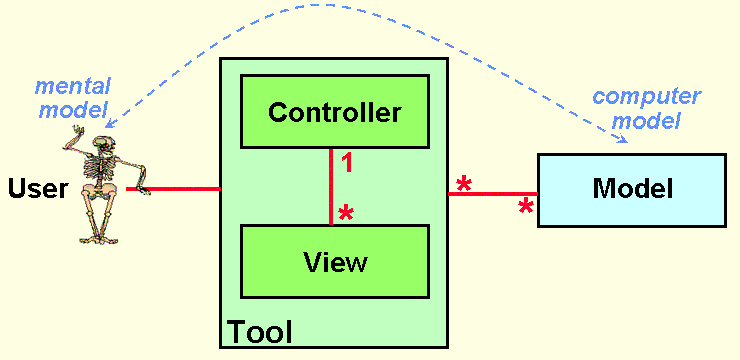
\includegraphics[width=\textwidth]{./images/chapter8/original_mvc}

This is a basic breakdown of the MVC pattern:

\begin{itemize}
\item Model - A model contains the data of the application.  
\item Controller - A controller interprets user input and transform it into a model that is represented to the user by the view.  The controller is responsible for processing user requests and building an appropriate model and passes it to the view for rendering. Here, the @Controller annotation is used to mark the class as the controller.
\item View - A view represents the provided information in a particular format.  Spring also supports view technologies such as Apache Velocity,  Thymeleaf and FreeMarker.
\end{itemize}

In Spring Web MVC,  we have this extra component, the DispatcherServlet class, which works as the front controller. It is responsible to manage the flow of the Spring MVC application.


\subsection{Views}

This section shows how Thymeleaf can be used as an template engine by Spring Boot.

First we add the dependency.

\begin{lstlisting}[frame=single]
<dependency>
	<groupId>org.springframework.boot</groupId>
	<artifactId>spring-boot-starter-thymeleaf</artifactId>
</dependency>
\end{lstlisting}

By default, Spring Boot looks for  templates in the directory src/main/resources/templates. 

We have two templates,  on for submitting a country name and a second for displaying the universities of the chosen country. 

\begin{lstlisting}[language=html, frame=single]
<!DOCTYPE html>
<html lang="en">
<head>
	<meta charset="UTF-8">
	<title>Search universities</title>
</head>
<body>
<form th:action="@{/universities}">
	<div>
		<label>Country:</label>
		<input type="text" th:name="country" />
	</div>
	<input type="submit"/>
</form>
</body>
</html>
\end{lstlisting}

\begin{lstlisting}[language=html, frame=single]
<!DOCTYPE html>
<html lang="en">
<head>
	<meta charset="UTF-8">
	<title>Title</title>
</head>
<body>
<div th:each="university : ${universities}">
	<a th:href="${university.webPages.get(0)}"><p th:text="${university.name}"></a>
</div>
</body>
</html>
\end{lstlisting}

Let's have a look at the controller.

\begin{lstlisting}[language=java, frame=single]
package be.pxl.paj.servlets.rest;

import be.pxl.paj.servlets.domain.University;
import org.springframework.stereotype.Controller;
import org.springframework.ui.Model;
import org.springframework.web.bind.annotation.GetMapping;
import org.springframework.web.bind.annotation.RequestMapping;
import org.springframework.web.bind.annotation.RequestParam;
import org.springframework.web.reactive.function.client.WebClient;

@Controller
public class UniversityController {

	private final WebClient webClient = WebClient.create("http://universities.hipolabs.com");

	@GetMapping("/country_selection")
	public String countrySelection() {
		return "country_selection";
	}

	@RequestMapping("/universities")
	public String addUser(@RequestParam(value = "country") String country, Model model) {
		WebClient.ResponseSpec response = webClient.get()
				.uri(String.format("search?country=%s", country))
				.retrieve();
		University[] universities = response.bodyToMono(University[].class).block();
		model.addAttribute("universities", universities);
		return "universities";
	}
}

\end{lstlisting}

The University class is a POJO-class.

\begin{lstlisting}[language=java, frame=single]
package be.pxl.paj.servlets.domain;

import com.fasterxml.jackson.annotation.JsonProperty;

import java.util.List;

public class University {
	private String name;
	@JsonProperty("web_pages")
	private List<String> webPages;

	public String getName() {
		return name;
	}

	public List<String> getWebPages() {
		return webPages;
	}
}
\end{lstlisting}


\section{@WebFilter}

Filters let you intercept the request.  And if you can intercept the request,
you can also control the response.  And, the servlet  never
knows that someone stepped in between the client request and the servlet container’s invocation 
of the servlet’s service() method.  Therefore,  if you choose to write and configure a filter, you're able to affect all of your servlets.  For example, if you want to add
user request tracking to every servlet in your application or manipulate the output
from every servlet? No problem.  Just write a filter and you don’t even have to touch the servlets.

\begin{lstlisting}[language=java, frame=single]
package be.pxl.paj.servlets;


import org.apache.logging.log4j.LogManager;
import org.apache.logging.log4j.Logger;

import jakarta.servlet.Filter;
import jakarta.servlet.FilterChain;
import jakarta.servlet.ServletException;
import jakarta.servlet.ServletRequest;
import jakarta.servlet.ServletResponse;
import jakarta.servlet.annotation.WebFilter;
import jakarta.servlet.http.HttpServletRequest;
import jakarta.servlet.http.HttpServletResponse;
import java.io.IOException;
import java.util.Collections;

@WebFilter(urlPatterns = { "/SelectBeer.do" })
public class HeaderLogFilter implements Filter {

	private static final Logger LOGGER = LogManager.getLogger(HeaderLogFilter.class);

	@Override
	public void doFilter(ServletRequest request, ServletResponse response,
	                     FilterChain chain) throws IOException, ServletException {
		HttpServletRequest req = (HttpServletRequest) request;
		HttpServletResponse rep = (HttpServletResponse) response;

		LOGGER.info("----- Request ---------");
		Collections.list(req.getHeaderNames()).forEach(n -> LOGGER.info(n + ": " + req.getHeader(n)));

		chain.doFilter(request, response);

		LOGGER.info("----- response ---------");

		rep.getHeaderNames().forEach(n -> LOGGER.info(n + ": " + rep.getHeader(n)));

		LOGGER.info("response status: " + rep.getStatus());
	}
}
\end{lstlisting}


\section{@WebListener}

@WebListener annotation is used to define a servlet listener component in a web application.

Many listeners are defined for events involving life cycles of ServletContext, HttpSession and ServletRequest.  Following listeners are supported for @WebListener:

\begin{itemize}
\item jakarta.servlet.ServletContextListener
\item jakarta.servlet.ServletContextAttributeListener
\item jakarta.servlet.ServletRequestListener
\item jakarta.servlet.ServletRequestAttributeListener
\item jakarta.servlet.http.HttpSessionListener
\item jakarta.servlet.http.HttpSessionAttributeListener
\end{itemize}


\begin{lstlisting}[language=java, frame=single]
package be.pxl.paj.servlets;

import jakarta.servlet.ServletContextEvent;
import jakarta.servlet.ServletContextListener;
import jakarta.servlet.annotation.WebListener;

@WebListener
public class ExampleContextListener implements ServletContextListener {

	@Override
	public void contextInitialized(ServletContextEvent servletContextEvent) {
		System.out.println("ServletDemo starting up!");
	}

	@Override
	public void contextDestroyed(ServletContextEvent servletContextEvent) {
		System.out.println("ServletDemo shutting down!");
	}
}
\end{lstlisting}

\section{Exercises}

\begin{oefening}
The html-page phonebook\_add.html is provided. Create a Servlet to handle the form’s POST request. The data is saved to a (in-memory) database. Make sure the phonenumber is unique.  Create a Servlet to display all the entries in the phonebook. 
\end{oefening}

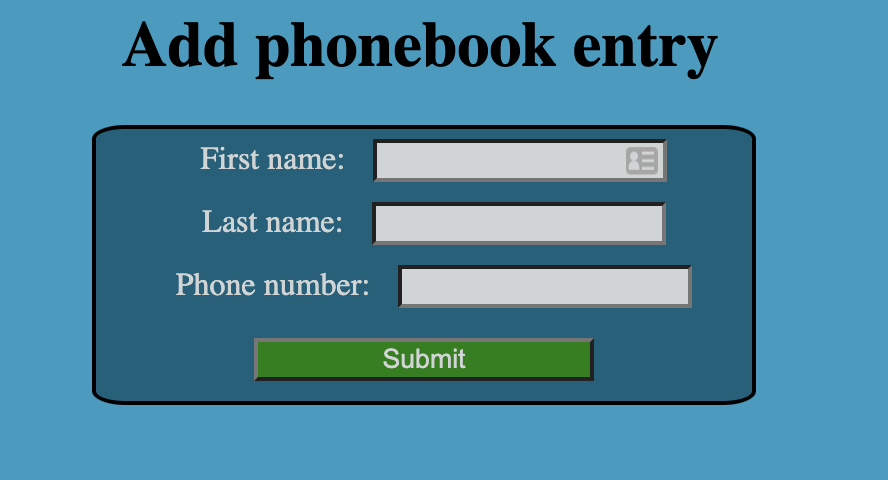
\includegraphics{./images/chapter8/add_phonebook_entry}


\chapter{Spring Data JPA Transaction management}

\fcolorbox{black}[HTML]{E9F0E9}{\parbox{\textwidth}{%
\noindent \textbf{Learning goals}\\
The junior-colleague
\begin{enumerate}[nolistsep]
\item can explain the ACID-properties of a transaction.
\item can implement transactions in spring boot applications.
\item can explain what a connection pool is.
\item can explain what transaction propagation is.
\item can explain the different possible transaction propagation methods.
\item can explain different isolation levels and the problems that can possibly occur.
\item can use flyway to implement database migrations.
\end{enumerate}}}

\section{Introduction}

A database transaction is a sequence of actions that are treated as a single unit of work. The actions should either complete entirely or take no effect at all. Transaction management is an important part of RDBMS-oriented enterprise application to ensure data integrity and consistency. The concept of transactions can be described with the following four key properties described as ACID \footnote{\url{https://www.youtube.com/watch?v=VRm2UMsFVz0}}:

\begin{itemize}
\item \textbf{Atomicity} A transaction should be treated as a single unit of operation, which means either the entire sequence of operations is successful or unsuccessful.

\item \textbf{Consistency} This represents the consistency of the referential integrity of the database, unique primary keys in tables, etc.

\item \textbf{Isolation} There may be many transaction processing with the same data set at the same time. Each transaction should be isolated from others to prevent data corruption.

\item \textbf{Durability} Once a transaction has completed, the results of this transaction have to be made permanent and cannot be erased from the database due to system failure.
\end{itemize}

If you are using a Spring Boot project and have a spring-data-* dependency on the classpath, then transaction management is enabled by default.

\section{Hikari connection pool}

\begin{verbatim}
HikariPool-1 - Starting...
HikariPool-1 - Added connection org.mariadb.jdbc.Connection@479111ba
HikariPool-1 - Start completed.
\end{verbatim}

Connection Pooling (CP) is the way to keep database connections open so that they can be reused by other clients (repositories), in other words, it is cache of database connections reused when future request to database is required. The application can access data at a faster rate, thereby reducing the number of database connections.
The default connection pool for Spring Boot applications is the Hikari Connection Pool (HikariCP).
Hikari-specific settings can be defined in the application.yml or application.properties file.

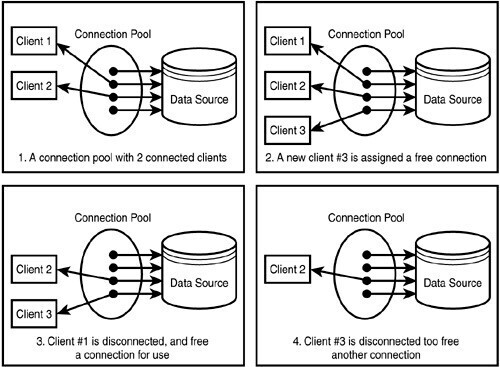
\includegraphics[width=\textwidth]{./images/chapter-tx/connection_pool.jpg}

\section{Transactions}

In most SpringBoot applications you will find two @Transactional annotations. One is provided by Spring the other is provided by JTA(Jakarta Transactional Annotations). They are in different packages. So when using the annotation make sure you know which one you have imported. We recommend using the one provided by Spring.

Just by using that annotation Spring does all the magic and we will not even be aware of what has happened.
You can always add the following properties to log the creation, commit and rollback of transactions.

\begin{verbatim}
logging.level.org.springframework.transaction.interceptor=trace
logging.level.org.springframework.orm.jpa=debug
logging.level.org.springframework.transaction=debug
\end{verbatim}

The @Transactional annotation is convenient because we as developers no longer need to think about how to start a transaction, how to execute it and when to do rollback or commit.

All of this is done automatically in a proxy class that Spring creates to hold the transaction management code. So yes, all those boilerplate codes are there but we just don’t see it. At run time, when the method annotated with @Transactional is called Spring, create a proxy class, in that proxy class it writes all the necessary codes to manage the transaction then it calls the actual class. to the logic and codes related to transactions is only done in the proxy class.

In its default configuration, the Spring Framework’s transaction infrastructure code marks a transaction for rollback only in the case of runtime, unchecked exceptions. That is, when the thrown exception is an instance or subclass of RuntimeException. (Error instances also, by default, result in a rollback). Checked exceptions that are thrown from a transactional method do not result in rollback in the default configuration.

\section{Transaction propagation}


Transaction propagation is the behavior of a transaction from one class to another. This means if class A has a method that creates a transaction and that method at some point has to call another transactional method in class B how should be the behavior of the method class B in regard to the transaction started by class A. And if there was no transaction started by class A what would class B do about that?

The possible transaction propagation methods are:

\begin{itemize}
\item \textbf{REQUIRED} This is the default propagation option. If a transaction already exists when a method annotated with REQUIRED is called, the method will execute within that transaction. If no transaction exists, a new transaction will be started.

\item \textbf{REQUIRES\_NEW} This option always starts a new transaction, even if a transaction already exists.

\item \textbf{SUPPORTS} This option allows a method to participate in a transaction if one already exists, but doesn’t start a new transaction if one doesn’t exist.

\item \textbf{MANDATORY} This option requires that a transaction already exists. If a transaction doesn’t exist, an exception is thrown.

\item \textbf{NOT\_SUPPORTED} This option specifies that a method should not participate in a transaction at all.

\item \textbf{NEVER} This option specifies that a method should never be called within a transaction.
\end{itemize}

More information: \url{https://dzone.com/articles/spring-transaction-propagation}

\url{https://www.geeksforgeeks.org/spring-boot-transaction-management-using-transactional-annotation/}

\section{Transaction isolation level}

Isolation determines how transaction integrity is visible to other users and systems.
Isolation levels define the degree to which a transaction must be isolated from the data modifications made by any other transaction in the database system. A transaction isolation level is defined by presence or absence of the following concurrency issues. 

\subsection{Concurrency Issues}

\subsubsection{Dirty Read}

A transaction reads the data that has not been committed by another transaction.

\includegraphics{./images/chapter-tx/DirtyRead.JPG}

\subsubsection{Lost Updates}

A lost update problem occurs due to the update of the same record by two different transactions at the same time. In simple words, when two transactions are updating the same record at the same time then a lost update problem occurs.

\includegraphics[width=\textwidth]{./images/chapter-tx/lost_update.png}

\subsubsection{Nonrepeatable Read}

Transaction reads the same row more than once and another transaction changes the data in the row between the successive reads of the transaction.

\includegraphics{./images/chapter-tx/NonRepeatable.JPG}

\subsubsection{Phantom Read}

A transaction reads a rowset more than once and another transaction inserts or deletes a row between the successive reads.

\includegraphics{./images/chapter-tx/PhantomRead.JPG}

\subsection{Setting Transaction Isolation Levels}

\includegraphics{./images/chapter-tx/isolation_level.png}

Isolation levels define the degree to which a transaction must be isolated from the data modifications made by any other transaction in the database system. 
Transaction isolation levels can improve concurrency by allowing multiple transactions to run concurrently without interfering with each other.


\subsubsection{Read Uncommitted}
In this level, a transaction can read the data modified by another transaction. But a transaction can read the data modified by another transaction even before the commit is made. Dirty Reads, Lost Updates, Nonrepeatable Read and Phantom read all issues occur at this level.

\subsubsection{Read Committed}
This is the default Isolation level in SQL database. In this level, When a transaction modifies a data other transactions will not be able to read the modified data. This prevents Dirty Reads but Lost Updates, Nonrepeatable Read and Phantom Read occurs at this level.

\subsubsection{Repeatable Read}
In this level, when a transaction is modifying data, no other transactions can read or ypdate the data until the current transaction completes it process. At this level, Dirty Reads, Lost Updates and Nonrepeatable Read are prevented but Phantom Read may occur.

\subsubsection{Serializable}
In this level, when a transaction is modifying data, no other transaction can read, update, modify or insert data until the current transaction completes its process and commits.


The default isolation level for Spring Boot application will be the default isolation of the RDBMS. MySQL and MariaDB's default isolation level is `Repeatable Read'. On the other hand, PostgreSQL and Oracle is `Read Committed'.


\section{Flyway}

Flyway is an open-source library used for Database Migration / Version Control for the DB scripts. It allows us to migrate the changes to DB incrementally by versioning.
Spring Boot provides easy integration with Flyway.


\begin{verbatim}
<dependency>
    <groupId>org.flywaydb</groupId>
    <artifactId>flyway-core</artifactId>
</dependency>
<dependency>
    <groupId>org.flywaydb</groupId>
    <artifactId>flyway-mysql</artifactId>
</dependency>
\end{verbatim}

The database migration are written in sql scripts. Make sure you follow the naming convention, otherwise the script will not be executed.

\includegraphics{./images/chapter-tx/flyway2.png}

Flyway creates a table flyway\_schema\_history where the current status of the database can be found.

\includegraphics[width=\textwidth]{./images/chapter-tx/flyway1.png}

An alternative for flyway is liquibase.








\chapter{Spring security}

\fcolorbox{black}[HTML]{E9F0E9}{\parbox{\textwidth}{%
\noindent \textbf{Learning goals}\\
The junior-colleague
\begin{enumerate}[nolistsep]
\item todo
\end{enumerate}
}}


\fcolorbox{black}[HTML]{ADD8E6}{\parbox{\textwidth}{%
\noindent \textbf{Source for this chapter:}\\
\url{https://github.com/custersnele/PAJ_Demo_MockMvcWithSecurity.git}
}}


\section{What is spring security}

\includegraphics[width=\textwidth]{./images/chapter-tx/spring_boot.png}

Spring Security is a framework that provides authentication, authorization, and protection against common attacks.

\section{JWT tokens}

\includegraphics[width=\textwidth]{./images/chapter-tx/JWT_request_response.png}

\section{Implementation}

\includegraphics[width=\textwidth]{./images/chapter-tx/spring-boot-security-jwt.png}

To enable HTTP Security in Spring, we need to create a SecurityFilterChain bean.


\textbf{WebSecurityConfig} holds all security implementation details. It configures cors, csrf, session management, rules for protected resources. We can also extend and customize the default configuration that contains the elements below.
WebSecurityConfig used to extend WebSecurityConfigurerAdapter, but WebSecurityConfigurerAdapter is deprecated from Spring 2.7.0.


\textbf{UserDetailsService} interface has a method to load User by username and returns a UserDetails object that Spring Security can use for authentication and validation.

\textbf{UserDetails} contains necessary information (such as: username, password, authorities) to build an Authentication object.

\textbf{UsernamePasswordAuthenticationToken} gets {username, password} from login Request, AuthenticationManager will use it to authenticate a login account.

\textbf{AuthenticationManager} has a DaoAuthenticationProvider (with help of UserDetailsService and PasswordEncoder) to validate UsernamePasswordAuthenticationToken object. If successful, AuthenticationManager returns a fully populated Authentication object (including granted authorities).

\textbf{OncePerRequestFilter} makes a single execution for each request to our API. It provides a doFilterInternal() method that we will implement parsing and validating JWT, loading User details (using UserDetailsService), checking Authorization (using UsernamePasswordAuthenticationToken).

\textbf{AuthController} handles login (and signup) requests.

You can enable security debugging as follows:

\begin{lstlisting}
@EnableWebSecurity(debug = true)
public class SecurityConfiguration {
...
}
\end{lstlisting}

\section{Unit tests}

With the @SpringBootTest annotation, Spring Boot provides a convenient way to start up an application context to be used in a test.

\begin{lstlisting}
@BeforeEach
void setup() {
	mockMvc = MockMvcBuilders
			.webAppContextSetup(context)
			.apply(SecurityMockMvcConfigurers.springSecurity())
			.build();
}
\end{lstlisting}

When using @SpringBootTest annotation to test controllers with Spring Security, it's necessary to explicitly configure the filter chain when setting up MockMvc.

Using the static springSecurity method provided by  SecurityMockMvcConfigurer is the preferred way to do this.

The annotation @WithMockUser is used to mock a logged-in user.

\section{Enabling Actuators, Metrics, and Health Indicators}

Actuator brings production-ready features to our application.
Monitoring our app, gathering metrics, understanding traffic, or the state of our database become possible with this dependency.
The main benefit of this library is that we can get production-grade tools without having to actually implement these features ourselves.

\begin{lstlisting}
<dependency>
	<groupId>org.springframework.boot</groupId>
	<artifactId>spring-boot-starter-actuator</artifactId>
</dependency>
\end{lstlisting}

Actuator comes with most endpoints disabled, to enable all endpoints use the following property:

\begin{verbatim}
management.endpoints.web.exposure.include=*
\end{verbatim}

As you can see, there are endpoints provided by the Spring Boot Actuator that expose important information about the application. Carefully evaluate the need to bring in spring-boot-stater-actuator and take steps to minimize the risk of security attacks.









TODO's

\begin{itemize}
\item can create a REST endpoint that provides an image or a file.
\item can run code analysis on a Spring boot project (with SonarQube).
\item can fix bugs, vulnerabilities and code smells detected by SonarQube.
\end{itemize}


\printbibliography



\end{document}
